\documentclass[twoside]{book}

% Packages required by doxygen
\usepackage{fixltx2e}
\usepackage{calc}
\usepackage{doxygen}
\usepackage[export]{adjustbox} % also loads graphicx
\usepackage{graphicx}
\usepackage[utf8]{inputenc}
\usepackage{makeidx}
\usepackage{multicol}
\usepackage{multirow}
\PassOptionsToPackage{warn}{textcomp}
\usepackage{textcomp}
\usepackage[nointegrals]{wasysym}
\usepackage[table]{xcolor}

% Font selection
\usepackage[T1]{fontenc}
\usepackage[scaled=.90]{helvet}
\usepackage{courier}
\usepackage{amssymb}
\usepackage{sectsty}
\renewcommand{\familydefault}{\sfdefault}
\allsectionsfont{%
  \fontseries{bc}\selectfont%
  \color{darkgray}%
}
\renewcommand{\DoxyLabelFont}{%
  \fontseries{bc}\selectfont%
  \color{darkgray}%
}
\newcommand{\+}{\discretionary{\mbox{\scriptsize$\hookleftarrow$}}{}{}}

% Page & text layout
\usepackage{geometry}
\geometry{%
  a4paper,%
  top=2.5cm,%
  bottom=2.5cm,%
  left=2.5cm,%
  right=2.5cm%
}
\tolerance=750
\hfuzz=15pt
\hbadness=750
\setlength{\emergencystretch}{15pt}
\setlength{\parindent}{0cm}
\setlength{\parskip}{3ex plus 2ex minus 2ex}
\makeatletter
\renewcommand{\paragraph}{%
  \@startsection{paragraph}{4}{0ex}{-1.0ex}{1.0ex}{%
    \normalfont\normalsize\bfseries\SS@parafont%
  }%
}
\renewcommand{\subparagraph}{%
  \@startsection{subparagraph}{5}{0ex}{-1.0ex}{1.0ex}{%
    \normalfont\normalsize\bfseries\SS@subparafont%
  }%
}
\makeatother

% Headers & footers
\usepackage{fancyhdr}
\pagestyle{fancyplain}
\fancyhead[LE]{\fancyplain{}{\bfseries\thepage}}
\fancyhead[CE]{\fancyplain{}{}}
\fancyhead[RE]{\fancyplain{}{\bfseries\leftmark}}
\fancyhead[LO]{\fancyplain{}{\bfseries\rightmark}}
\fancyhead[CO]{\fancyplain{}{}}
\fancyhead[RO]{\fancyplain{}{\bfseries\thepage}}
\fancyfoot[LE]{\fancyplain{}{}}
\fancyfoot[CE]{\fancyplain{}{}}
\fancyfoot[RE]{\fancyplain{}{\bfseries\scriptsize Generated by Doxygen }}
\fancyfoot[LO]{\fancyplain{}{\bfseries\scriptsize Generated by Doxygen }}
\fancyfoot[CO]{\fancyplain{}{}}
\fancyfoot[RO]{\fancyplain{}{}}
\renewcommand{\footrulewidth}{0.4pt}
\renewcommand{\chaptermark}[1]{%
  \markboth{#1}{}%
}
\renewcommand{\sectionmark}[1]{%
  \markright{\thesection\ #1}%
}

% Indices & bibliography
\usepackage{natbib}
\usepackage[titles]{tocloft}
\setcounter{tocdepth}{3}
\setcounter{secnumdepth}{5}
\makeindex

% Hyperlinks (required, but should be loaded last)
\usepackage{ifpdf}
\ifpdf
  \usepackage[pdftex,pagebackref=true]{hyperref}
\else
  \usepackage[ps2pdf,pagebackref=true]{hyperref}
\fi
\hypersetup{%
  colorlinks=true,%
  linkcolor=blue,%
  citecolor=blue,%
  unicode%
}

% Custom commands
\newcommand{\clearemptydoublepage}{%
  \newpage{\pagestyle{empty}\cleardoublepage}%
}

\usepackage{caption}
\captionsetup{labelsep=space,justification=centering,font={bf},singlelinecheck=off,skip=4pt,position=top}

%===== C O N T E N T S =====

\begin{document}

% Titlepage & ToC
\hypersetup{pageanchor=false,
             bookmarksnumbered=true,
             pdfencoding=unicode
            }
\pagenumbering{alph}
\begin{titlepage}
\vspace*{7cm}
\begin{center}%
{\Large Project Codename Olympia }\\
\vspace*{1cm}
{\large Generated by Doxygen 1.8.13}\\
\end{center}
\end{titlepage}
\clearemptydoublepage
\pagenumbering{roman}
\tableofcontents
\clearemptydoublepage
\pagenumbering{arabic}
\hypersetup{pageanchor=true}

%--- Begin generated contents ---
\chapter{Namespace Index}
\section{Namespace List}
Here is a list of all documented namespaces with brief descriptions\+:\begin{DoxyCompactList}
\item\contentsline{section}{\hyperlink{namespaceProject__Codename__Olympia__v1}{Project\+\_\+\+Codename\+\_\+\+Olympia\+\_\+v1} }{\pageref{namespaceProject__Codename__Olympia__v1}}{}
\item\contentsline{section}{\hyperlink{namespaceProject__Codename__Olympia__v1_1_1__0}{Project\+\_\+\+Codename\+\_\+\+Olympia\+\_\+v1.\+\_\+0} }{\pageref{namespaceProject__Codename__Olympia__v1_1_1__0}}{}
\end{DoxyCompactList}

\chapter{Hierarchical Index}
\section{Class Hierarchy}
This inheritance list is sorted roughly, but not completely, alphabetically\+:\begin{DoxyCompactList}
\item \contentsline{section}{Athlete}{\pageref{classAthlete}}{}
\item \contentsline{section}{Database}{\pageref{classDatabase}}{}
\item Form\begin{DoxyCompactList}
\item \contentsline{section}{P\+C\+O.\+\_\+0.\+Athlete\+Form}{\pageref{classPCO_1_1__0_1_1AthleteForm}}{}
\item \contentsline{section}{P\+C\+O.\+\_\+0.\+Display}{\pageref{classPCO_1_1__0_1_1Display}}{}
\item \contentsline{section}{P\+C\+O.\+\_\+0.\+Form1}{\pageref{classPCO_1_1__0_1_1Form1}}{}
\item \contentsline{section}{P\+C\+O.\+\_\+0.\+Register\+Event\+Form}{\pageref{classPCO_1_1__0_1_1RegisterEventForm}}{}
\item \contentsline{section}{P\+C\+O.\+\_\+0.\+Scoring\+Form}{\pageref{classPCO_1_1__0_1_1ScoringForm}}{}
\item \contentsline{section}{P\+C\+O.\+\_\+0.\+Team\+Form}{\pageref{classPCO_1_1__0_1_1TeamForm}}{}
\end{DoxyCompactList}
\item \contentsline{section}{Ice\+Dance}{\pageref{classIceDance}}{}
\item \contentsline{section}{Pair\+Skating}{\pageref{classPairSkating}}{}
\item \contentsline{section}{Registration}{\pageref{classRegistration}}{}
\item \contentsline{section}{Scoring}{\pageref{classScoring}}{}
\item \contentsline{section}{Single\+Skating}{\pageref{classSingleSkating}}{}
\item \contentsline{section}{S\+S1000m}{\pageref{classSS1000m}}{}
\item \contentsline{section}{S\+S1500m}{\pageref{classSS1500m}}{}
\item \contentsline{section}{S\+S500m}{\pageref{classSS500m}}{}
\item \contentsline{section}{Team}{\pageref{classTeam}}{}
\end{DoxyCompactList}

\chapter{Class Index}
\section{Class List}
Here are the classes, structs, unions and interfaces with brief descriptions\+:\begin{DoxyCompactList}
\item\contentsline{section}{\hyperlink{classPCO_1_1Athlete}{P\+C\+O.\+Athlete} \\*\hyperlink{classPCO_1_1Athlete}{Athlete} class to input individual's personal information and events to partake in }{\pageref{classPCO_1_1Athlete}}{}
\item\contentsline{section}{\hyperlink{classPCO_1_1Database}{P\+C\+O.\+Database} \\*D\+E\+P\+R\+E\+C\+A\+T\+E\+D!!! \hyperlink{classPCO_1_1Database}{Database} S\+U\+B\+S\+Y\+S\+T\+E\+M houses all the information of the Winter Olympics }{\pageref{classPCO_1_1Database}}{}
\item\contentsline{section}{\hyperlink{classPCO_1_1Event}{P\+C\+O.\+Event} \\*\hyperlink{classPCO_1_1Event}{Event} class is the superclass of all the 2 event types and 6 specific events }{\pageref{classPCO_1_1Event}}{}
\item\contentsline{section}{\hyperlink{interfacePCO_1_1Event_1_1eventInheritance}{P\+C\+O.\+Event.\+event\+Inheritance} }{\pageref{interfacePCO_1_1Event_1_1eventInheritance}}{}
\item\contentsline{section}{\hyperlink{classPCO_1_1FigureSkating}{P\+C\+O.\+Figure\+Skating} \\*\hyperlink{classPCO_1_1FigureSkating}{Figure\+Skating} class is the superclass of the 3 \hyperlink{classPCO_1_1FigureSkating}{Figure\+Skating} events }{\pageref{classPCO_1_1FigureSkating}}{}
\item\contentsline{section}{\hyperlink{interfacePCO_1_1FigureSkating_1_1fsInheritance}{P\+C\+O.\+Figure\+Skating.\+fs\+Inheritance} }{\pageref{interfacePCO_1_1FigureSkating_1_1fsInheritance}}{}
\item\contentsline{section}{\hyperlink{classPCO_1_1IceDance}{P\+C\+O.\+Ice\+Dance} \\*\hyperlink{classPCO_1_1IceDance}{Ice\+Dance} class is one of the 3 \hyperlink{classPCO_1_1FigureSkating}{Figure\+Skating} events }{\pageref{classPCO_1_1IceDance}}{}
\item\contentsline{section}{\hyperlink{classPCO_1_1Judge}{P\+C\+O.\+Judge} \\*\hyperlink{classPCO_1_1Judge}{Judge} class houses and disperses all the qualified judges }{\pageref{classPCO_1_1Judge}}{}
\item\contentsline{section}{\hyperlink{classPCO_1_1MainClass}{P\+C\+O.\+Main\+Class} }{\pageref{classPCO_1_1MainClass}}{}
\item\contentsline{section}{\hyperlink{classPCO_1_1PairSkating}{P\+C\+O.\+Pair\+Skating} \\*\hyperlink{classPCO_1_1PairSkating}{Pair\+Skating} class is one of the 3 \hyperlink{classPCO_1_1FigureSkating}{Figure\+Skating} events }{\pageref{classPCO_1_1PairSkating}}{}
\item\contentsline{section}{\hyperlink{classPCO_1_1Registration}{P\+C\+O.\+Registration} \\*\hyperlink{classPCO_1_1Registration}{Registration} class registers Teams and Athletes }{\pageref{classPCO_1_1Registration}}{}
\item\contentsline{section}{\hyperlink{classPCO_1_1Rink}{P\+C\+O.\+Rink} \\*\hyperlink{classPCO_1_1Rink}{Rink} class is the physical area in which events are held }{\pageref{classPCO_1_1Rink}}{}
\item\contentsline{section}{\hyperlink{classPCO_1_1Schedule}{P\+C\+O.\+Schedule} \\*\hyperlink{classPCO_1_1Schedule}{Schedule} class is the organization of athletes and events }{\pageref{classPCO_1_1Schedule}}{}
\item\contentsline{section}{\hyperlink{classPCO_1_1Scoring}{P\+C\+O.\+Scoring} \\*\hyperlink{classPCO_1_1Scoring}{Scoring} class manages the official scores/times recorded by the judges }{\pageref{classPCO_1_1Scoring}}{}
\item\contentsline{section}{\hyperlink{classPCO_1_1SingleSkating}{P\+C\+O.\+Single\+Skating} \\*\hyperlink{classPCO_1_1SingleSkating}{Single\+Skating} class is one of the 3 \hyperlink{classPCO_1_1FigureSkating}{Figure\+Skating} events }{\pageref{classPCO_1_1SingleSkating}}{}
\item\contentsline{section}{\hyperlink{classPCO_1_1SpeedSkating}{P\+C\+O.\+Speed\+Skating} \\*\hyperlink{classPCO_1_1SpeedSkating}{Speed\+Skating} class is the superclass of the 3 \hyperlink{classPCO_1_1SpeedSkating}{Speed\+Skating} events }{\pageref{classPCO_1_1SpeedSkating}}{}
\item\contentsline{section}{\hyperlink{classPCO_1_1SS1000m}{P\+C\+O.\+S\+S1000m} \\*\hyperlink{classPCO_1_1SS1000m}{S\+S1000m} is one of the 3 \hyperlink{classPCO_1_1SpeedSkating}{Speed\+Skating} events }{\pageref{classPCO_1_1SS1000m}}{}
\item\contentsline{section}{\hyperlink{classPCO_1_1SS1500m}{P\+C\+O.\+S\+S1500m} \\*\hyperlink{classPCO_1_1SS1500m}{S\+S1500m} is one of the 3 \hyperlink{classPCO_1_1SpeedSkating}{Speed\+Skating} events }{\pageref{classPCO_1_1SS1500m}}{}
\item\contentsline{section}{\hyperlink{classPCO_1_1SS500m}{P\+C\+O.\+S\+S500m} \\*\hyperlink{classPCO_1_1SS500m}{S\+S500m} is one of the 3 \hyperlink{classPCO_1_1SpeedSkating}{Speed\+Skating} events }{\pageref{classPCO_1_1SS500m}}{}
\item\contentsline{section}{\hyperlink{interfacePCO_1_1SpeedSkating_1_1ssInheritance}{P\+C\+O.\+Speed\+Skating.\+ss\+Inheritance} }{\pageref{interfacePCO_1_1SpeedSkating_1_1ssInheritance}}{}
\item\contentsline{section}{\hyperlink{classPCO_1_1Team}{P\+C\+O.\+Team} \\*\hyperlink{classPCO_1_1Team}{Team} class to house the team name }{\pageref{classPCO_1_1Team}}{}
\end{DoxyCompactList}

\chapter{File Index}
\section{File List}
Here is a list of all files with brief descriptions\+:\begin{DoxyCompactList}
\item\contentsline{section}{\hyperlink{Class1_8cs}{Class1.\+cs} }{\pageref{Class1_8cs}}{}
\item\contentsline{section}{\hyperlink{Display_8cs}{Display.\+cs} }{\pageref{Display_8cs}}{}
\item\contentsline{section}{\hyperlink{Display_8Designer_8cs}{Display.\+Designer.\+cs} }{\pageref{Display_8Designer_8cs}}{}
\item\contentsline{section}{\hyperlink{Event_8cs}{Event.\+cs} }{\pageref{Event_8cs}}{}
\item\contentsline{section}{\hyperlink{Event_8Designer_8cs}{Event.\+Designer.\+cs} }{\pageref{Event_8Designer_8cs}}{}
\item\contentsline{section}{\hyperlink{Form1_8cs}{Form1.\+cs} }{\pageref{Form1_8cs}}{}
\item\contentsline{section}{\hyperlink{Form1_8Designer_8cs}{Form1.\+Designer.\+cs} }{\pageref{Form1_8Designer_8cs}}{}
\item\contentsline{section}{\hyperlink{Judge_8cs}{Judge.\+cs} }{\pageref{Judge_8cs}}{}
\item\contentsline{section}{\hyperlink{Judge_8Designer_8cs}{Judge.\+Designer.\+cs} }{\pageref{Judge_8Designer_8cs}}{}
\item\contentsline{section}{\hyperlink{Program_8cs}{Program.\+cs} }{\pageref{Program_8cs}}{}
\item\contentsline{section}{\hyperlink{Registration_8cs}{Registration.\+cs} }{\pageref{Registration_8cs}}{}
\item\contentsline{section}{\hyperlink{Registration_8Designer_8cs}{Registration.\+Designer.\+cs} }{\pageref{Registration_8Designer_8cs}}{}
\item\contentsline{section}{\hyperlink{Team_8cs}{Team.\+cs} }{\pageref{Team_8cs}}{}
\item\contentsline{section}{\hyperlink{Team_8Designer_8cs}{Team.\+Designer.\+cs} }{\pageref{Team_8Designer_8cs}}{}
\end{DoxyCompactList}

\chapter{Namespace Documentation}
\hypertarget{namespacePCO}{\section{Package P\+C\+O}
\label{namespacePCO}\index{P\+C\+O@{P\+C\+O}}
}
\subsection*{Classes}
\begin{DoxyCompactItemize}
\item 
class \hyperlink{classPCO_1_1Athlete}{Athlete}
\begin{DoxyCompactList}\small\item\em \hyperlink{classPCO_1_1Athlete}{Athlete} class to input individual's personal information and events to partake in. \end{DoxyCompactList}\item 
class \hyperlink{classPCO_1_1Database}{Database}
\begin{DoxyCompactList}\small\item\em D\+E\+P\+R\+E\+C\+A\+T\+E\+D!!! \hyperlink{classPCO_1_1Database}{Database} S\+U\+B\+S\+Y\+S\+T\+E\+M houses all the information of the Winter Olympics. \end{DoxyCompactList}\item 
class \hyperlink{classPCO_1_1Event}{Event}
\begin{DoxyCompactList}\small\item\em \hyperlink{classPCO_1_1Event}{Event} class is the superclass of all the 2 event types and 6 specific events. \end{DoxyCompactList}\item 
class \hyperlink{classPCO_1_1FigureSkating}{Figure\+Skating}
\begin{DoxyCompactList}\small\item\em \hyperlink{classPCO_1_1FigureSkating}{Figure\+Skating} class is the superclass of the 3 \hyperlink{classPCO_1_1FigureSkating}{Figure\+Skating} events. \end{DoxyCompactList}\item 
class \hyperlink{classPCO_1_1IceDance}{Ice\+Dance}
\begin{DoxyCompactList}\small\item\em \hyperlink{classPCO_1_1IceDance}{Ice\+Dance} class is one of the 3 \hyperlink{classPCO_1_1FigureSkating}{Figure\+Skating} events. \end{DoxyCompactList}\item 
class \hyperlink{classPCO_1_1Judge}{Judge}
\begin{DoxyCompactList}\small\item\em \hyperlink{classPCO_1_1Judge}{Judge} class houses and disperses all the qualified judges. \end{DoxyCompactList}\item 
class \hyperlink{classPCO_1_1MainClass}{Main\+Class}
\item 
class \hyperlink{classPCO_1_1PairSkating}{Pair\+Skating}
\begin{DoxyCompactList}\small\item\em \hyperlink{classPCO_1_1PairSkating}{Pair\+Skating} class is one of the 3 \hyperlink{classPCO_1_1FigureSkating}{Figure\+Skating} events. \end{DoxyCompactList}\item 
class \hyperlink{classPCO_1_1Registration}{Registration}
\begin{DoxyCompactList}\small\item\em \hyperlink{classPCO_1_1Registration}{Registration} class registers Teams and Athletes. \end{DoxyCompactList}\item 
class \hyperlink{classPCO_1_1Rink}{Rink}
\begin{DoxyCompactList}\small\item\em \hyperlink{classPCO_1_1Rink}{Rink} class is the physical area in which events are held. \end{DoxyCompactList}\item 
class \hyperlink{classPCO_1_1Schedule}{Schedule}
\begin{DoxyCompactList}\small\item\em \hyperlink{classPCO_1_1Schedule}{Schedule} class is the organization of athletes and events. \end{DoxyCompactList}\item 
class \hyperlink{classPCO_1_1Scoring}{Scoring}
\begin{DoxyCompactList}\small\item\em \hyperlink{classPCO_1_1Scoring}{Scoring} class manages the official scores/times recorded by the judges. \end{DoxyCompactList}\item 
class \hyperlink{classPCO_1_1SingleSkating}{Single\+Skating}
\begin{DoxyCompactList}\small\item\em \hyperlink{classPCO_1_1SingleSkating}{Single\+Skating} class is one of the 3 \hyperlink{classPCO_1_1FigureSkating}{Figure\+Skating} events. \end{DoxyCompactList}\item 
class \hyperlink{classPCO_1_1SpeedSkating}{Speed\+Skating}
\begin{DoxyCompactList}\small\item\em \hyperlink{classPCO_1_1SpeedSkating}{Speed\+Skating} class is the superclass of the 3 \hyperlink{classPCO_1_1SpeedSkating}{Speed\+Skating} events. \end{DoxyCompactList}\item 
class \hyperlink{classPCO_1_1SS1000m}{S\+S1000m}
\begin{DoxyCompactList}\small\item\em \hyperlink{classPCO_1_1SS1000m}{S\+S1000m} is one of the 3 \hyperlink{classPCO_1_1SpeedSkating}{Speed\+Skating} events. \end{DoxyCompactList}\item 
class \hyperlink{classPCO_1_1SS1500m}{S\+S1500m}
\begin{DoxyCompactList}\small\item\em \hyperlink{classPCO_1_1SS1500m}{S\+S1500m} is one of the 3 \hyperlink{classPCO_1_1SpeedSkating}{Speed\+Skating} events. \end{DoxyCompactList}\item 
class \hyperlink{classPCO_1_1SS500m}{S\+S500m}
\begin{DoxyCompactList}\small\item\em \hyperlink{classPCO_1_1SS500m}{S\+S500m} is one of the 3 \hyperlink{classPCO_1_1SpeedSkating}{Speed\+Skating} events. \end{DoxyCompactList}\item 
class \hyperlink{classPCO_1_1Team}{Team}
\begin{DoxyCompactList}\small\item\em \hyperlink{classPCO_1_1Team}{Team} class to house the team name. \end{DoxyCompactList}\end{DoxyCompactItemize}

\hypertarget{namespacePCO_1_1__0}{}\section{P\+C\+O.\+\_\+0 Namespace Reference}
\label{namespacePCO_1_1__0}\index{P\+C\+O.\+\_\+0@{P\+C\+O.\+\_\+0}}
\subsection*{Classes}
\begin{DoxyCompactItemize}
\item 
class \hyperlink{classPCO_1_1__0_1_1AthleteForm}{Athlete\+Form}
\begin{DoxyCompactList}\small\item\em \hyperlink{classRegistration}{Registration} class for G\+UI. \end{DoxyCompactList}\item 
class \hyperlink{classPCO_1_1__0_1_1Display}{Display}
\begin{DoxyCompactList}\small\item\em \hyperlink{classPCO_1_1__0_1_1Display}{Display} class for G\+UI. \end{DoxyCompactList}\item 
class \hyperlink{classPCO_1_1__0_1_1Form1}{Form1}
\begin{DoxyCompactList}\small\item\em Main Screen class for G\+UI. \end{DoxyCompactList}\item 
class {\bfseries Program}
\item 
class \hyperlink{classPCO_1_1__0_1_1RegisterEventForm}{Register\+Event\+Form}
\begin{DoxyCompactList}\small\item\em Register Event class for G\+UI. \end{DoxyCompactList}\item 
class \hyperlink{classPCO_1_1__0_1_1ScoringForm}{Scoring\+Form}
\begin{DoxyCompactList}\small\item\em \hyperlink{classScoring}{Scoring} class for G\+UI. \end{DoxyCompactList}\item 
class \hyperlink{classPCO_1_1__0_1_1TeamForm}{Team\+Form}
\begin{DoxyCompactList}\small\item\em \hyperlink{classTeam}{Team} class for G\+UI. \end{DoxyCompactList}\end{DoxyCompactItemize}

\chapter{Class Documentation}
\hypertarget{classAthlete}{}\section{Athlete Class Reference}
\label{classAthlete}\index{Athlete@{Athlete}}


\hyperlink{classAthlete}{Athlete} class to input individual\textquotesingle{}s personal information and events to partake in.  


\subsection*{Public Member Functions}
\begin{DoxyCompactItemize}
\item 
\hyperlink{classAthlete_a3b2ab137b0f940eee2965898bd22dadb}{Athlete} ()
\end{DoxyCompactItemize}
\subsection*{Properties}
\begin{DoxyCompactItemize}
\item 
string \hyperlink{classAthlete_af1567abd99a20dd128959681ef7f457b}{first\+Name}\hspace{0.3cm}{\ttfamily  \mbox{[}get, set\mbox{]}}
\item 
string \hyperlink{classAthlete_a9d8f08579c9749c7f40965a100fc8b08}{last\+Name}\hspace{0.3cm}{\ttfamily  \mbox{[}get, set\mbox{]}}
\item 
string \hyperlink{classAthlete_a6606f4bf491738676ed79d3680bbe1b2}{gender}\hspace{0.3cm}{\ttfamily  \mbox{[}get, set\mbox{]}}
\end{DoxyCompactItemize}


\subsection{Detailed Description}
\hyperlink{classAthlete}{Athlete} class to input individual\textquotesingle{}s personal information and events to partake in. 

D\+E\+F\+I\+N\+I\+T\+I\+ON\+: An individual who is a part of a team in the Winter Olympics.

C\+O\+N\+S\+T\+R\+A\+I\+N\+TS\+: Can only be registered if maximum allotted space on their respective team has not been reached. This also includes the gender portion.\begin{DoxyAuthor}{Author}
Landen Marchand 
\end{DoxyAuthor}


Definition at line 24 of file Class1.\+cs.



\subsection{Constructor \& Destructor Documentation}
\mbox{\Hypertarget{classAthlete_a3b2ab137b0f940eee2965898bd22dadb}\label{classAthlete_a3b2ab137b0f940eee2965898bd22dadb}} 
\index{Athlete@{Athlete}!Athlete@{Athlete}}
\index{Athlete@{Athlete}!Athlete@{Athlete}}
\subsubsection{\texorpdfstring{Athlete()}{Athlete()}}
{\footnotesize\ttfamily Athlete.\+Athlete (\begin{DoxyParamCaption}{ }\end{DoxyParamCaption})\hspace{0.3cm}{\ttfamily [inline]}}

Default Constructor Provided Automatically 
\begin{DoxyParams}{Parameters}
{\em None} & \\
\hline
\end{DoxyParams}
\begin{DoxyReturn}{Returns}
Default Values 
\end{DoxyReturn}


Definition at line 30 of file Class1.\+cs.



\subsection{Property Documentation}
\mbox{\Hypertarget{classAthlete_af1567abd99a20dd128959681ef7f457b}\label{classAthlete_af1567abd99a20dd128959681ef7f457b}} 
\index{Athlete@{Athlete}!first\+Name@{first\+Name}}
\index{first\+Name@{first\+Name}!Athlete@{Athlete}}
\subsubsection{\texorpdfstring{first\+Name}{firstName}}
{\footnotesize\ttfamily string Athlete.\+first\+Name\hspace{0.3cm}{\ttfamily [get]}, {\ttfamily [set]}}

Sets and gets athlete\textquotesingle{}s first name 
\begin{DoxyParams}{Parameters}
{\em string} & for first name \\
\hline
\end{DoxyParams}
\begin{DoxyReturn}{Returns}
string of first name 
\end{DoxyReturn}


Definition at line 39 of file Class1.\+cs.

\mbox{\Hypertarget{classAthlete_a6606f4bf491738676ed79d3680bbe1b2}\label{classAthlete_a6606f4bf491738676ed79d3680bbe1b2}} 
\index{Athlete@{Athlete}!gender@{gender}}
\index{gender@{gender}!Athlete@{Athlete}}
\subsubsection{\texorpdfstring{gender}{gender}}
{\footnotesize\ttfamily string Athlete.\+gender\hspace{0.3cm}{\ttfamily [get]}, {\ttfamily [set]}}

Sets and gets athlete\textquotesingle{}s gender 
\begin{DoxyParams}{Parameters}
{\em string} & for gender \\
\hline
\end{DoxyParams}
\begin{DoxyReturn}{Returns}
string of gender 
\end{DoxyReturn}


Definition at line 49 of file Class1.\+cs.

\mbox{\Hypertarget{classAthlete_a9d8f08579c9749c7f40965a100fc8b08}\label{classAthlete_a9d8f08579c9749c7f40965a100fc8b08}} 
\index{Athlete@{Athlete}!last\+Name@{last\+Name}}
\index{last\+Name@{last\+Name}!Athlete@{Athlete}}
\subsubsection{\texorpdfstring{last\+Name}{lastName}}
{\footnotesize\ttfamily string Athlete.\+last\+Name\hspace{0.3cm}{\ttfamily [get]}, {\ttfamily [set]}}

Sets and gets athlete\textquotesingle{}s last name 
\begin{DoxyParams}{Parameters}
{\em string} & for last name \\
\hline
\end{DoxyParams}
\begin{DoxyReturn}{Returns}
string of last name 
\end{DoxyReturn}


Definition at line 44 of file Class1.\+cs.



The documentation for this class was generated from the following file\+:\begin{DoxyCompactItemize}
\item 
\hyperlink{Class1_8cs}{Class1.\+cs}\end{DoxyCompactItemize}

\hypertarget{classPCO_1_1__0_1_1AthleteForm}{}\section{P\+C\+O.\+\_\+0.\+Athlete\+Form Class Reference}
\label{classPCO_1_1__0_1_1AthleteForm}\index{P\+C\+O.\+\_\+0.\+Athlete\+Form@{P\+C\+O.\+\_\+0.\+Athlete\+Form}}


\hyperlink{classRegistration}{Registration} class for G\+UI.  




Inheritance diagram for P\+C\+O.\+\_\+0.\+Athlete\+Form\+:\nopagebreak
\begin{figure}[H]
\begin{center}
\leavevmode
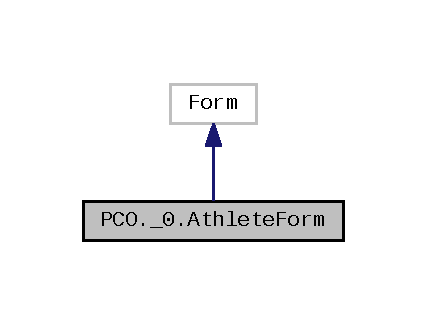
\includegraphics[width=205pt]{classPCO_1_1__0_1_1AthleteForm__inherit__graph}
\end{center}
\end{figure}


Collaboration diagram for P\+C\+O.\+\_\+0.\+Athlete\+Form\+:\nopagebreak
\begin{figure}[H]
\begin{center}
\leavevmode
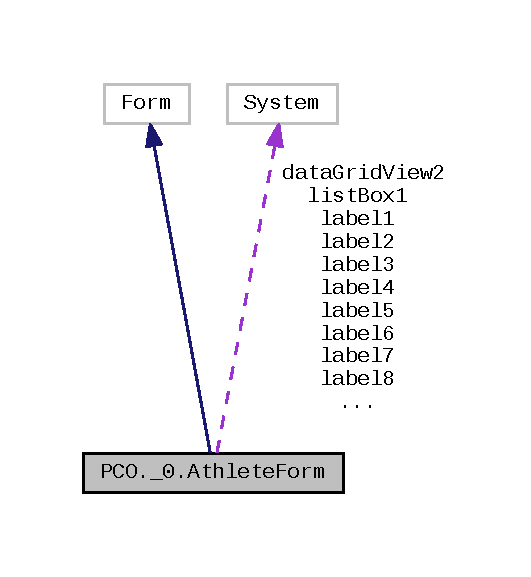
\includegraphics[width=255pt]{classPCO_1_1__0_1_1AthleteForm__coll__graph}
\end{center}
\end{figure}
\subsection*{Public Member Functions}
\begin{DoxyCompactItemize}
\item 
\hyperlink{classPCO_1_1__0_1_1AthleteForm_a3a129c00c114ef80d97231dfa01e2d6f}{Athlete\+Form} ()
\end{DoxyCompactItemize}
\subsection*{Protected Member Functions}
\begin{DoxyCompactItemize}
\item 
override void \hyperlink{classPCO_1_1__0_1_1AthleteForm_a28a1dc2c4ccd788db94afe809d281df3}{Dispose} (bool disposing)
\begin{DoxyCompactList}\small\item\em Clean up any resources being used. \end{DoxyCompactList}\end{DoxyCompactItemize}
\subsection*{Private Member Functions}
\begin{DoxyCompactItemize}
\item 
void \hyperlink{classPCO_1_1__0_1_1AthleteForm_adb6a10dd23db479964768b71cac7c6e2}{Athlete\+Form\+\_\+\+Load} (object sender, Event\+Args e)
\item 
void \hyperlink{classPCO_1_1__0_1_1AthleteForm_a00446a6a149c1afa1a7c8e4b6b4fc14a}{list\+Box1\+\_\+\+Selected\+Index\+Changed} (object sender, Event\+Args e)
\item 
void \hyperlink{classPCO_1_1__0_1_1AthleteForm_a0ec9eb6075e62e7d5b376b681e171414}{button1\+\_\+\+Click} (object sender, Event\+Args e)
\item 
void \hyperlink{classPCO_1_1__0_1_1AthleteForm_aae4000b1be563d683ade5454b2c88349}{button2\+\_\+\+Click} (object sender, Event\+Args e)
\item 
void \hyperlink{classPCO_1_1__0_1_1AthleteForm_afb260385ed6476b844cdc357bf11df25}{button3\+\_\+\+Click} (object sender, Event\+Args e)
\item 
void \hyperlink{classPCO_1_1__0_1_1AthleteForm_aa5ce4e96e22a27bed4a483bb549c2619}{Initialize\+Component} ()
\begin{DoxyCompactList}\small\item\em Required method for Designer support -\/ do not modify the contents of this method with the code editor. \end{DoxyCompactList}\end{DoxyCompactItemize}
\subsection*{Private Attributes}
\begin{DoxyCompactItemize}
\item 
System.\+Component\+Model.\+I\+Container \hyperlink{classPCO_1_1__0_1_1AthleteForm_a1f16b28e2014bb3d3819173c19fba17e}{components} = null
\begin{DoxyCompactList}\small\item\em Required designer variable. \end{DoxyCompactList}\item 
System.\+Windows.\+Forms.\+Text\+Box \hyperlink{classPCO_1_1__0_1_1AthleteForm_a1e440213d1900de946894fdff1854cd0}{text\+Box1}
\item 
System.\+Windows.\+Forms.\+Label \hyperlink{classPCO_1_1__0_1_1AthleteForm_abe2a3d915a0c7b22f4f5b81230ad8278}{label1}
\item 
System.\+Windows.\+Forms.\+Text\+Box \hyperlink{classPCO_1_1__0_1_1AthleteForm_a2099ea4a6adbe82e58e924892ba3154d}{text\+Box2}
\item 
System.\+Windows.\+Forms.\+Label \hyperlink{classPCO_1_1__0_1_1AthleteForm_af0c25b3c3b035069efd110610a46e91c}{label2}
\item 
System.\+Windows.\+Forms.\+List\+Box \hyperlink{classPCO_1_1__0_1_1AthleteForm_a0564d30b38ba13222cf51a999a972421}{list\+Box1}
\item 
System.\+Windows.\+Forms.\+Label \hyperlink{classPCO_1_1__0_1_1AthleteForm_a8a41e84122bfaf6f2aecc58f2f016e83}{label4}
\item 
System.\+Windows.\+Forms.\+Data\+Grid\+View \hyperlink{classPCO_1_1__0_1_1AthleteForm_ae32ac29356b096ba9f5e22ba20b58348}{data\+Grid\+View1}
\item 
System.\+Windows.\+Forms.\+Button \hyperlink{classPCO_1_1__0_1_1AthleteForm_acabccda502389ae2d4d220140b058b79}{button1}
\item 
System.\+Windows.\+Forms.\+Label \hyperlink{classPCO_1_1__0_1_1AthleteForm_a916d83226b3339f4c9f084b225e5c4f2}{label5}
\item 
System.\+Windows.\+Forms.\+Data\+Grid\+View \hyperlink{classPCO_1_1__0_1_1AthleteForm_a7f4664bac19be7add32755591473e803}{data\+Grid\+View2}
\item 
System.\+Windows.\+Forms.\+Label \hyperlink{classPCO_1_1__0_1_1AthleteForm_a9d417f399c88183f59ea21d20f0ecf6f}{label6}
\item 
System.\+Windows.\+Forms.\+Label \hyperlink{classPCO_1_1__0_1_1AthleteForm_a06304d0926cac7dffedc7e77cd224555}{label3}
\item 
System.\+Windows.\+Forms.\+Label \hyperlink{classPCO_1_1__0_1_1AthleteForm_ae3cc01074736dd8511ca37fbd2ac55e4}{label7}
\item 
System.\+Windows.\+Forms.\+Button \hyperlink{classPCO_1_1__0_1_1AthleteForm_a7c8166ff30baadd6cb0c281cd8308e30}{button2}
\item 
System.\+Windows.\+Forms.\+Button \hyperlink{classPCO_1_1__0_1_1AthleteForm_a6dc6a58f8577a62db3b3b767ddcb5b04}{button3}
\item 
System.\+Windows.\+Forms.\+Label \hyperlink{classPCO_1_1__0_1_1AthleteForm_a1813ffa0b4fd481ad8934a606ed413d6}{label8}
\item 
System.\+Windows.\+Forms.\+Label \hyperlink{classPCO_1_1__0_1_1AthleteForm_ad04e7a32bf0bd1ea170cd962becc8c94}{label9}
\end{DoxyCompactItemize}


\subsection{Detailed Description}
\hyperlink{classRegistration}{Registration} class for G\+UI. 

Definition at line 16 of file Registration.\+cs.



\subsection{Constructor \& Destructor Documentation}
\mbox{\Hypertarget{classPCO_1_1__0_1_1AthleteForm_a3a129c00c114ef80d97231dfa01e2d6f}\label{classPCO_1_1__0_1_1AthleteForm_a3a129c00c114ef80d97231dfa01e2d6f}} 
\index{P\+C\+O\+::\+\_\+0\+::\+Athlete\+Form@{P\+C\+O\+::\+\_\+0\+::\+Athlete\+Form}!Athlete\+Form@{Athlete\+Form}}
\index{Athlete\+Form@{Athlete\+Form}!P\+C\+O\+::\+\_\+0\+::\+Athlete\+Form@{P\+C\+O\+::\+\_\+0\+::\+Athlete\+Form}}
\subsubsection{\texorpdfstring{Athlete\+Form()}{AthleteForm()}}
{\footnotesize\ttfamily P\+C\+O.\+\_\+0.\+Athlete\+Form.\+Athlete\+Form (\begin{DoxyParamCaption}{ }\end{DoxyParamCaption})\hspace{0.3cm}{\ttfamily [inline]}}



Definition at line 18 of file Registration.\+cs.



\subsection{Member Function Documentation}
\mbox{\Hypertarget{classPCO_1_1__0_1_1AthleteForm_adb6a10dd23db479964768b71cac7c6e2}\label{classPCO_1_1__0_1_1AthleteForm_adb6a10dd23db479964768b71cac7c6e2}} 
\index{P\+C\+O\+::\+\_\+0\+::\+Athlete\+Form@{P\+C\+O\+::\+\_\+0\+::\+Athlete\+Form}!Athlete\+Form\+\_\+\+Load@{Athlete\+Form\+\_\+\+Load}}
\index{Athlete\+Form\+\_\+\+Load@{Athlete\+Form\+\_\+\+Load}!P\+C\+O\+::\+\_\+0\+::\+Athlete\+Form@{P\+C\+O\+::\+\_\+0\+::\+Athlete\+Form}}
\subsubsection{\texorpdfstring{Athlete\+Form\+\_\+\+Load()}{AthleteForm\_Load()}}
{\footnotesize\ttfamily void P\+C\+O.\+\_\+0.\+Athlete\+Form.\+Athlete\+Form\+\_\+\+Load (\begin{DoxyParamCaption}\item[{object}]{sender,  }\item[{Event\+Args}]{e }\end{DoxyParamCaption})\hspace{0.3cm}{\ttfamily [inline]}, {\ttfamily [private]}}



Definition at line 23 of file Registration.\+cs.

\mbox{\Hypertarget{classPCO_1_1__0_1_1AthleteForm_a0ec9eb6075e62e7d5b376b681e171414}\label{classPCO_1_1__0_1_1AthleteForm_a0ec9eb6075e62e7d5b376b681e171414}} 
\index{P\+C\+O\+::\+\_\+0\+::\+Athlete\+Form@{P\+C\+O\+::\+\_\+0\+::\+Athlete\+Form}!button1\+\_\+\+Click@{button1\+\_\+\+Click}}
\index{button1\+\_\+\+Click@{button1\+\_\+\+Click}!P\+C\+O\+::\+\_\+0\+::\+Athlete\+Form@{P\+C\+O\+::\+\_\+0\+::\+Athlete\+Form}}
\subsubsection{\texorpdfstring{button1\+\_\+\+Click()}{button1\_Click()}}
{\footnotesize\ttfamily void P\+C\+O.\+\_\+0.\+Athlete\+Form.\+button1\+\_\+\+Click (\begin{DoxyParamCaption}\item[{object}]{sender,  }\item[{Event\+Args}]{e }\end{DoxyParamCaption})\hspace{0.3cm}{\ttfamily [inline]}, {\ttfamily [private]}}



Definition at line 81 of file Registration.\+cs.

\mbox{\Hypertarget{classPCO_1_1__0_1_1AthleteForm_aae4000b1be563d683ade5454b2c88349}\label{classPCO_1_1__0_1_1AthleteForm_aae4000b1be563d683ade5454b2c88349}} 
\index{P\+C\+O\+::\+\_\+0\+::\+Athlete\+Form@{P\+C\+O\+::\+\_\+0\+::\+Athlete\+Form}!button2\+\_\+\+Click@{button2\+\_\+\+Click}}
\index{button2\+\_\+\+Click@{button2\+\_\+\+Click}!P\+C\+O\+::\+\_\+0\+::\+Athlete\+Form@{P\+C\+O\+::\+\_\+0\+::\+Athlete\+Form}}
\subsubsection{\texorpdfstring{button2\+\_\+\+Click()}{button2\_Click()}}
{\footnotesize\ttfamily void P\+C\+O.\+\_\+0.\+Athlete\+Form.\+button2\+\_\+\+Click (\begin{DoxyParamCaption}\item[{object}]{sender,  }\item[{Event\+Args}]{e }\end{DoxyParamCaption})\hspace{0.3cm}{\ttfamily [inline]}, {\ttfamily [private]}}



Definition at line 128 of file Registration.\+cs.

\mbox{\Hypertarget{classPCO_1_1__0_1_1AthleteForm_afb260385ed6476b844cdc357bf11df25}\label{classPCO_1_1__0_1_1AthleteForm_afb260385ed6476b844cdc357bf11df25}} 
\index{P\+C\+O\+::\+\_\+0\+::\+Athlete\+Form@{P\+C\+O\+::\+\_\+0\+::\+Athlete\+Form}!button3\+\_\+\+Click@{button3\+\_\+\+Click}}
\index{button3\+\_\+\+Click@{button3\+\_\+\+Click}!P\+C\+O\+::\+\_\+0\+::\+Athlete\+Form@{P\+C\+O\+::\+\_\+0\+::\+Athlete\+Form}}
\subsubsection{\texorpdfstring{button3\+\_\+\+Click()}{button3\_Click()}}
{\footnotesize\ttfamily void P\+C\+O.\+\_\+0.\+Athlete\+Form.\+button3\+\_\+\+Click (\begin{DoxyParamCaption}\item[{object}]{sender,  }\item[{Event\+Args}]{e }\end{DoxyParamCaption})\hspace{0.3cm}{\ttfamily [inline]}, {\ttfamily [private]}}



Definition at line 164 of file Registration.\+cs.

\mbox{\Hypertarget{classPCO_1_1__0_1_1AthleteForm_a28a1dc2c4ccd788db94afe809d281df3}\label{classPCO_1_1__0_1_1AthleteForm_a28a1dc2c4ccd788db94afe809d281df3}} 
\index{P\+C\+O\+::\+\_\+0\+::\+Athlete\+Form@{P\+C\+O\+::\+\_\+0\+::\+Athlete\+Form}!Dispose@{Dispose}}
\index{Dispose@{Dispose}!P\+C\+O\+::\+\_\+0\+::\+Athlete\+Form@{P\+C\+O\+::\+\_\+0\+::\+Athlete\+Form}}
\subsubsection{\texorpdfstring{Dispose()}{Dispose()}}
{\footnotesize\ttfamily override void P\+C\+O.\+\_\+0.\+Athlete\+Form.\+Dispose (\begin{DoxyParamCaption}\item[{bool}]{disposing }\end{DoxyParamCaption})\hspace{0.3cm}{\ttfamily [inline]}, {\ttfamily [protected]}}



Clean up any resources being used. 


\begin{DoxyParams}{Parameters}
{\em disposing} & true if managed resources should be disposed; otherwise, false.\\
\hline
\end{DoxyParams}


Definition at line 14 of file Registration.\+Designer.\+cs.

\mbox{\Hypertarget{classPCO_1_1__0_1_1AthleteForm_aa5ce4e96e22a27bed4a483bb549c2619}\label{classPCO_1_1__0_1_1AthleteForm_aa5ce4e96e22a27bed4a483bb549c2619}} 
\index{P\+C\+O\+::\+\_\+0\+::\+Athlete\+Form@{P\+C\+O\+::\+\_\+0\+::\+Athlete\+Form}!Initialize\+Component@{Initialize\+Component}}
\index{Initialize\+Component@{Initialize\+Component}!P\+C\+O\+::\+\_\+0\+::\+Athlete\+Form@{P\+C\+O\+::\+\_\+0\+::\+Athlete\+Form}}
\subsubsection{\texorpdfstring{Initialize\+Component()}{InitializeComponent()}}
{\footnotesize\ttfamily void P\+C\+O.\+\_\+0.\+Athlete\+Form.\+Initialize\+Component (\begin{DoxyParamCaption}{ }\end{DoxyParamCaption})\hspace{0.3cm}{\ttfamily [inline]}, {\ttfamily [private]}}



Required method for Designer support -\/ do not modify the contents of this method with the code editor. 



Definition at line 29 of file Registration.\+Designer.\+cs.

\mbox{\Hypertarget{classPCO_1_1__0_1_1AthleteForm_a00446a6a149c1afa1a7c8e4b6b4fc14a}\label{classPCO_1_1__0_1_1AthleteForm_a00446a6a149c1afa1a7c8e4b6b4fc14a}} 
\index{P\+C\+O\+::\+\_\+0\+::\+Athlete\+Form@{P\+C\+O\+::\+\_\+0\+::\+Athlete\+Form}!list\+Box1\+\_\+\+Selected\+Index\+Changed@{list\+Box1\+\_\+\+Selected\+Index\+Changed}}
\index{list\+Box1\+\_\+\+Selected\+Index\+Changed@{list\+Box1\+\_\+\+Selected\+Index\+Changed}!P\+C\+O\+::\+\_\+0\+::\+Athlete\+Form@{P\+C\+O\+::\+\_\+0\+::\+Athlete\+Form}}
\subsubsection{\texorpdfstring{list\+Box1\+\_\+\+Selected\+Index\+Changed()}{listBox1\_SelectedIndexChanged()}}
{\footnotesize\ttfamily void P\+C\+O.\+\_\+0.\+Athlete\+Form.\+list\+Box1\+\_\+\+Selected\+Index\+Changed (\begin{DoxyParamCaption}\item[{object}]{sender,  }\item[{Event\+Args}]{e }\end{DoxyParamCaption})\hspace{0.3cm}{\ttfamily [inline]}, {\ttfamily [private]}}



Definition at line 76 of file Registration.\+cs.



\subsection{Member Data Documentation}
\mbox{\Hypertarget{classPCO_1_1__0_1_1AthleteForm_acabccda502389ae2d4d220140b058b79}\label{classPCO_1_1__0_1_1AthleteForm_acabccda502389ae2d4d220140b058b79}} 
\index{P\+C\+O\+::\+\_\+0\+::\+Athlete\+Form@{P\+C\+O\+::\+\_\+0\+::\+Athlete\+Form}!button1@{button1}}
\index{button1@{button1}!P\+C\+O\+::\+\_\+0\+::\+Athlete\+Form@{P\+C\+O\+::\+\_\+0\+::\+Athlete\+Form}}
\subsubsection{\texorpdfstring{button1}{button1}}
{\footnotesize\ttfamily System.\+Windows.\+Forms.\+Button P\+C\+O.\+\_\+0.\+Athlete\+Form.\+button1\hspace{0.3cm}{\ttfamily [private]}}



Definition at line 245 of file Registration.\+Designer.\+cs.

\mbox{\Hypertarget{classPCO_1_1__0_1_1AthleteForm_a7c8166ff30baadd6cb0c281cd8308e30}\label{classPCO_1_1__0_1_1AthleteForm_a7c8166ff30baadd6cb0c281cd8308e30}} 
\index{P\+C\+O\+::\+\_\+0\+::\+Athlete\+Form@{P\+C\+O\+::\+\_\+0\+::\+Athlete\+Form}!button2@{button2}}
\index{button2@{button2}!P\+C\+O\+::\+\_\+0\+::\+Athlete\+Form@{P\+C\+O\+::\+\_\+0\+::\+Athlete\+Form}}
\subsubsection{\texorpdfstring{button2}{button2}}
{\footnotesize\ttfamily System.\+Windows.\+Forms.\+Button P\+C\+O.\+\_\+0.\+Athlete\+Form.\+button2\hspace{0.3cm}{\ttfamily [private]}}



Definition at line 251 of file Registration.\+Designer.\+cs.

\mbox{\Hypertarget{classPCO_1_1__0_1_1AthleteForm_a6dc6a58f8577a62db3b3b767ddcb5b04}\label{classPCO_1_1__0_1_1AthleteForm_a6dc6a58f8577a62db3b3b767ddcb5b04}} 
\index{P\+C\+O\+::\+\_\+0\+::\+Athlete\+Form@{P\+C\+O\+::\+\_\+0\+::\+Athlete\+Form}!button3@{button3}}
\index{button3@{button3}!P\+C\+O\+::\+\_\+0\+::\+Athlete\+Form@{P\+C\+O\+::\+\_\+0\+::\+Athlete\+Form}}
\subsubsection{\texorpdfstring{button3}{button3}}
{\footnotesize\ttfamily System.\+Windows.\+Forms.\+Button P\+C\+O.\+\_\+0.\+Athlete\+Form.\+button3\hspace{0.3cm}{\ttfamily [private]}}



Definition at line 252 of file Registration.\+Designer.\+cs.

\mbox{\Hypertarget{classPCO_1_1__0_1_1AthleteForm_a1f16b28e2014bb3d3819173c19fba17e}\label{classPCO_1_1__0_1_1AthleteForm_a1f16b28e2014bb3d3819173c19fba17e}} 
\index{P\+C\+O\+::\+\_\+0\+::\+Athlete\+Form@{P\+C\+O\+::\+\_\+0\+::\+Athlete\+Form}!components@{components}}
\index{components@{components}!P\+C\+O\+::\+\_\+0\+::\+Athlete\+Form@{P\+C\+O\+::\+\_\+0\+::\+Athlete\+Form}}
\subsubsection{\texorpdfstring{components}{components}}
{\footnotesize\ttfamily System.\+Component\+Model.\+I\+Container P\+C\+O.\+\_\+0.\+Athlete\+Form.\+components = null\hspace{0.3cm}{\ttfamily [private]}}



Required designer variable. 



Definition at line 8 of file Registration.\+Designer.\+cs.

\mbox{\Hypertarget{classPCO_1_1__0_1_1AthleteForm_ae32ac29356b096ba9f5e22ba20b58348}\label{classPCO_1_1__0_1_1AthleteForm_ae32ac29356b096ba9f5e22ba20b58348}} 
\index{P\+C\+O\+::\+\_\+0\+::\+Athlete\+Form@{P\+C\+O\+::\+\_\+0\+::\+Athlete\+Form}!data\+Grid\+View1@{data\+Grid\+View1}}
\index{data\+Grid\+View1@{data\+Grid\+View1}!P\+C\+O\+::\+\_\+0\+::\+Athlete\+Form@{P\+C\+O\+::\+\_\+0\+::\+Athlete\+Form}}
\subsubsection{\texorpdfstring{data\+Grid\+View1}{dataGridView1}}
{\footnotesize\ttfamily System.\+Windows.\+Forms.\+Data\+Grid\+View P\+C\+O.\+\_\+0.\+Athlete\+Form.\+data\+Grid\+View1\hspace{0.3cm}{\ttfamily [private]}}



Definition at line 244 of file Registration.\+Designer.\+cs.

\mbox{\Hypertarget{classPCO_1_1__0_1_1AthleteForm_a7f4664bac19be7add32755591473e803}\label{classPCO_1_1__0_1_1AthleteForm_a7f4664bac19be7add32755591473e803}} 
\index{P\+C\+O\+::\+\_\+0\+::\+Athlete\+Form@{P\+C\+O\+::\+\_\+0\+::\+Athlete\+Form}!data\+Grid\+View2@{data\+Grid\+View2}}
\index{data\+Grid\+View2@{data\+Grid\+View2}!P\+C\+O\+::\+\_\+0\+::\+Athlete\+Form@{P\+C\+O\+::\+\_\+0\+::\+Athlete\+Form}}
\subsubsection{\texorpdfstring{data\+Grid\+View2}{dataGridView2}}
{\footnotesize\ttfamily System.\+Windows.\+Forms.\+Data\+Grid\+View P\+C\+O.\+\_\+0.\+Athlete\+Form.\+data\+Grid\+View2\hspace{0.3cm}{\ttfamily [private]}}



Definition at line 247 of file Registration.\+Designer.\+cs.

\mbox{\Hypertarget{classPCO_1_1__0_1_1AthleteForm_abe2a3d915a0c7b22f4f5b81230ad8278}\label{classPCO_1_1__0_1_1AthleteForm_abe2a3d915a0c7b22f4f5b81230ad8278}} 
\index{P\+C\+O\+::\+\_\+0\+::\+Athlete\+Form@{P\+C\+O\+::\+\_\+0\+::\+Athlete\+Form}!label1@{label1}}
\index{label1@{label1}!P\+C\+O\+::\+\_\+0\+::\+Athlete\+Form@{P\+C\+O\+::\+\_\+0\+::\+Athlete\+Form}}
\subsubsection{\texorpdfstring{label1}{label1}}
{\footnotesize\ttfamily System.\+Windows.\+Forms.\+Label P\+C\+O.\+\_\+0.\+Athlete\+Form.\+label1\hspace{0.3cm}{\ttfamily [private]}}



Definition at line 239 of file Registration.\+Designer.\+cs.

\mbox{\Hypertarget{classPCO_1_1__0_1_1AthleteForm_af0c25b3c3b035069efd110610a46e91c}\label{classPCO_1_1__0_1_1AthleteForm_af0c25b3c3b035069efd110610a46e91c}} 
\index{P\+C\+O\+::\+\_\+0\+::\+Athlete\+Form@{P\+C\+O\+::\+\_\+0\+::\+Athlete\+Form}!label2@{label2}}
\index{label2@{label2}!P\+C\+O\+::\+\_\+0\+::\+Athlete\+Form@{P\+C\+O\+::\+\_\+0\+::\+Athlete\+Form}}
\subsubsection{\texorpdfstring{label2}{label2}}
{\footnotesize\ttfamily System.\+Windows.\+Forms.\+Label P\+C\+O.\+\_\+0.\+Athlete\+Form.\+label2\hspace{0.3cm}{\ttfamily [private]}}



Definition at line 241 of file Registration.\+Designer.\+cs.

\mbox{\Hypertarget{classPCO_1_1__0_1_1AthleteForm_a06304d0926cac7dffedc7e77cd224555}\label{classPCO_1_1__0_1_1AthleteForm_a06304d0926cac7dffedc7e77cd224555}} 
\index{P\+C\+O\+::\+\_\+0\+::\+Athlete\+Form@{P\+C\+O\+::\+\_\+0\+::\+Athlete\+Form}!label3@{label3}}
\index{label3@{label3}!P\+C\+O\+::\+\_\+0\+::\+Athlete\+Form@{P\+C\+O\+::\+\_\+0\+::\+Athlete\+Form}}
\subsubsection{\texorpdfstring{label3}{label3}}
{\footnotesize\ttfamily System.\+Windows.\+Forms.\+Label P\+C\+O.\+\_\+0.\+Athlete\+Form.\+label3\hspace{0.3cm}{\ttfamily [private]}}



Definition at line 249 of file Registration.\+Designer.\+cs.

\mbox{\Hypertarget{classPCO_1_1__0_1_1AthleteForm_a8a41e84122bfaf6f2aecc58f2f016e83}\label{classPCO_1_1__0_1_1AthleteForm_a8a41e84122bfaf6f2aecc58f2f016e83}} 
\index{P\+C\+O\+::\+\_\+0\+::\+Athlete\+Form@{P\+C\+O\+::\+\_\+0\+::\+Athlete\+Form}!label4@{label4}}
\index{label4@{label4}!P\+C\+O\+::\+\_\+0\+::\+Athlete\+Form@{P\+C\+O\+::\+\_\+0\+::\+Athlete\+Form}}
\subsubsection{\texorpdfstring{label4}{label4}}
{\footnotesize\ttfamily System.\+Windows.\+Forms.\+Label P\+C\+O.\+\_\+0.\+Athlete\+Form.\+label4\hspace{0.3cm}{\ttfamily [private]}}



Definition at line 243 of file Registration.\+Designer.\+cs.

\mbox{\Hypertarget{classPCO_1_1__0_1_1AthleteForm_a916d83226b3339f4c9f084b225e5c4f2}\label{classPCO_1_1__0_1_1AthleteForm_a916d83226b3339f4c9f084b225e5c4f2}} 
\index{P\+C\+O\+::\+\_\+0\+::\+Athlete\+Form@{P\+C\+O\+::\+\_\+0\+::\+Athlete\+Form}!label5@{label5}}
\index{label5@{label5}!P\+C\+O\+::\+\_\+0\+::\+Athlete\+Form@{P\+C\+O\+::\+\_\+0\+::\+Athlete\+Form}}
\subsubsection{\texorpdfstring{label5}{label5}}
{\footnotesize\ttfamily System.\+Windows.\+Forms.\+Label P\+C\+O.\+\_\+0.\+Athlete\+Form.\+label5\hspace{0.3cm}{\ttfamily [private]}}



Definition at line 246 of file Registration.\+Designer.\+cs.

\mbox{\Hypertarget{classPCO_1_1__0_1_1AthleteForm_a9d417f399c88183f59ea21d20f0ecf6f}\label{classPCO_1_1__0_1_1AthleteForm_a9d417f399c88183f59ea21d20f0ecf6f}} 
\index{P\+C\+O\+::\+\_\+0\+::\+Athlete\+Form@{P\+C\+O\+::\+\_\+0\+::\+Athlete\+Form}!label6@{label6}}
\index{label6@{label6}!P\+C\+O\+::\+\_\+0\+::\+Athlete\+Form@{P\+C\+O\+::\+\_\+0\+::\+Athlete\+Form}}
\subsubsection{\texorpdfstring{label6}{label6}}
{\footnotesize\ttfamily System.\+Windows.\+Forms.\+Label P\+C\+O.\+\_\+0.\+Athlete\+Form.\+label6\hspace{0.3cm}{\ttfamily [private]}}



Definition at line 248 of file Registration.\+Designer.\+cs.

\mbox{\Hypertarget{classPCO_1_1__0_1_1AthleteForm_ae3cc01074736dd8511ca37fbd2ac55e4}\label{classPCO_1_1__0_1_1AthleteForm_ae3cc01074736dd8511ca37fbd2ac55e4}} 
\index{P\+C\+O\+::\+\_\+0\+::\+Athlete\+Form@{P\+C\+O\+::\+\_\+0\+::\+Athlete\+Form}!label7@{label7}}
\index{label7@{label7}!P\+C\+O\+::\+\_\+0\+::\+Athlete\+Form@{P\+C\+O\+::\+\_\+0\+::\+Athlete\+Form}}
\subsubsection{\texorpdfstring{label7}{label7}}
{\footnotesize\ttfamily System.\+Windows.\+Forms.\+Label P\+C\+O.\+\_\+0.\+Athlete\+Form.\+label7\hspace{0.3cm}{\ttfamily [private]}}



Definition at line 250 of file Registration.\+Designer.\+cs.

\mbox{\Hypertarget{classPCO_1_1__0_1_1AthleteForm_a1813ffa0b4fd481ad8934a606ed413d6}\label{classPCO_1_1__0_1_1AthleteForm_a1813ffa0b4fd481ad8934a606ed413d6}} 
\index{P\+C\+O\+::\+\_\+0\+::\+Athlete\+Form@{P\+C\+O\+::\+\_\+0\+::\+Athlete\+Form}!label8@{label8}}
\index{label8@{label8}!P\+C\+O\+::\+\_\+0\+::\+Athlete\+Form@{P\+C\+O\+::\+\_\+0\+::\+Athlete\+Form}}
\subsubsection{\texorpdfstring{label8}{label8}}
{\footnotesize\ttfamily System.\+Windows.\+Forms.\+Label P\+C\+O.\+\_\+0.\+Athlete\+Form.\+label8\hspace{0.3cm}{\ttfamily [private]}}



Definition at line 253 of file Registration.\+Designer.\+cs.

\mbox{\Hypertarget{classPCO_1_1__0_1_1AthleteForm_ad04e7a32bf0bd1ea170cd962becc8c94}\label{classPCO_1_1__0_1_1AthleteForm_ad04e7a32bf0bd1ea170cd962becc8c94}} 
\index{P\+C\+O\+::\+\_\+0\+::\+Athlete\+Form@{P\+C\+O\+::\+\_\+0\+::\+Athlete\+Form}!label9@{label9}}
\index{label9@{label9}!P\+C\+O\+::\+\_\+0\+::\+Athlete\+Form@{P\+C\+O\+::\+\_\+0\+::\+Athlete\+Form}}
\subsubsection{\texorpdfstring{label9}{label9}}
{\footnotesize\ttfamily System.\+Windows.\+Forms.\+Label P\+C\+O.\+\_\+0.\+Athlete\+Form.\+label9\hspace{0.3cm}{\ttfamily [private]}}



Definition at line 254 of file Registration.\+Designer.\+cs.

\mbox{\Hypertarget{classPCO_1_1__0_1_1AthleteForm_a0564d30b38ba13222cf51a999a972421}\label{classPCO_1_1__0_1_1AthleteForm_a0564d30b38ba13222cf51a999a972421}} 
\index{P\+C\+O\+::\+\_\+0\+::\+Athlete\+Form@{P\+C\+O\+::\+\_\+0\+::\+Athlete\+Form}!list\+Box1@{list\+Box1}}
\index{list\+Box1@{list\+Box1}!P\+C\+O\+::\+\_\+0\+::\+Athlete\+Form@{P\+C\+O\+::\+\_\+0\+::\+Athlete\+Form}}
\subsubsection{\texorpdfstring{list\+Box1}{listBox1}}
{\footnotesize\ttfamily System.\+Windows.\+Forms.\+List\+Box P\+C\+O.\+\_\+0.\+Athlete\+Form.\+list\+Box1\hspace{0.3cm}{\ttfamily [private]}}



Definition at line 242 of file Registration.\+Designer.\+cs.

\mbox{\Hypertarget{classPCO_1_1__0_1_1AthleteForm_a1e440213d1900de946894fdff1854cd0}\label{classPCO_1_1__0_1_1AthleteForm_a1e440213d1900de946894fdff1854cd0}} 
\index{P\+C\+O\+::\+\_\+0\+::\+Athlete\+Form@{P\+C\+O\+::\+\_\+0\+::\+Athlete\+Form}!text\+Box1@{text\+Box1}}
\index{text\+Box1@{text\+Box1}!P\+C\+O\+::\+\_\+0\+::\+Athlete\+Form@{P\+C\+O\+::\+\_\+0\+::\+Athlete\+Form}}
\subsubsection{\texorpdfstring{text\+Box1}{textBox1}}
{\footnotesize\ttfamily System.\+Windows.\+Forms.\+Text\+Box P\+C\+O.\+\_\+0.\+Athlete\+Form.\+text\+Box1\hspace{0.3cm}{\ttfamily [private]}}



Definition at line 238 of file Registration.\+Designer.\+cs.

\mbox{\Hypertarget{classPCO_1_1__0_1_1AthleteForm_a2099ea4a6adbe82e58e924892ba3154d}\label{classPCO_1_1__0_1_1AthleteForm_a2099ea4a6adbe82e58e924892ba3154d}} 
\index{P\+C\+O\+::\+\_\+0\+::\+Athlete\+Form@{P\+C\+O\+::\+\_\+0\+::\+Athlete\+Form}!text\+Box2@{text\+Box2}}
\index{text\+Box2@{text\+Box2}!P\+C\+O\+::\+\_\+0\+::\+Athlete\+Form@{P\+C\+O\+::\+\_\+0\+::\+Athlete\+Form}}
\subsubsection{\texorpdfstring{text\+Box2}{textBox2}}
{\footnotesize\ttfamily System.\+Windows.\+Forms.\+Text\+Box P\+C\+O.\+\_\+0.\+Athlete\+Form.\+text\+Box2\hspace{0.3cm}{\ttfamily [private]}}



Definition at line 240 of file Registration.\+Designer.\+cs.



The documentation for this class was generated from the following files\+:\begin{DoxyCompactItemize}
\item 
\hyperlink{Registration_8cs}{Registration.\+cs}\item 
\hyperlink{Registration_8Designer_8cs}{Registration.\+Designer.\+cs}\end{DoxyCompactItemize}

\hypertarget{classDatabase}{}\section{Database Class Reference}
\label{classDatabase}\index{Database@{Database}}


D\+E\+P\+R\+E\+C\+A\+T\+E\+D!!! \hyperlink{classDatabase}{Database} S\+U\+B\+S\+Y\+S\+T\+EM houses all the information of the Winter Olympics.  


\subsection*{Public Member Functions}
\begin{DoxyCompactItemize}
\item 
\hyperlink{classDatabase_a2ed32b5fa1ed9b2591c32ddcda28e337}{Database} ()
\end{DoxyCompactItemize}


\subsection{Detailed Description}
D\+E\+P\+R\+E\+C\+A\+T\+E\+D!!! \hyperlink{classDatabase}{Database} S\+U\+B\+S\+Y\+S\+T\+EM houses all the information of the Winter Olympics. 

D\+E\+F\+I\+N\+I\+T\+I\+ON\+: The collection of all information for all events in the Winter Olympics. A database also is a collection of all registrants information.

C\+O\+N\+S\+T\+R\+A\+I\+N\+TS\+: Must contain information apropos to the event and registrants at hand.\begin{DoxyAuthor}{Author}
Landen Marchand 
\end{DoxyAuthor}


Definition at line 59 of file Class1.\+cs.



\subsection{Constructor \& Destructor Documentation}
\mbox{\Hypertarget{classDatabase_a2ed32b5fa1ed9b2591c32ddcda28e337}\label{classDatabase_a2ed32b5fa1ed9b2591c32ddcda28e337}} 
\index{Database@{Database}!Database@{Database}}
\index{Database@{Database}!Database@{Database}}
\subsubsection{\texorpdfstring{Database()}{Database()}}
{\footnotesize\ttfamily Database.\+Database (\begin{DoxyParamCaption}{ }\end{DoxyParamCaption})\hspace{0.3cm}{\ttfamily [inline]}}



Definition at line 61 of file Class1.\+cs.



The documentation for this class was generated from the following file\+:\begin{DoxyCompactItemize}
\item 
\hyperlink{Class1_8cs}{Class1.\+cs}\end{DoxyCompactItemize}

\hypertarget{classPCO_1_1__0_1_1Display}{}\section{P\+C\+O.\+\_\+0.\+Display Class Reference}
\label{classPCO_1_1__0_1_1Display}\index{P\+C\+O.\+\_\+0.\+Display@{P\+C\+O.\+\_\+0.\+Display}}


\hyperlink{classPCO_1_1__0_1_1Display}{Display} class for G\+UI.  




Inheritance diagram for P\+C\+O.\+\_\+0.\+Display\+:\nopagebreak
\begin{figure}[H]
\begin{center}
\leavevmode
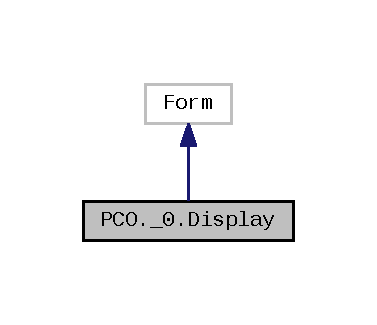
\includegraphics[width=181pt]{classPCO_1_1__0_1_1Display__inherit__graph}
\end{center}
\end{figure}


Collaboration diagram for P\+C\+O.\+\_\+0.\+Display\+:\nopagebreak
\begin{figure}[H]
\begin{center}
\leavevmode
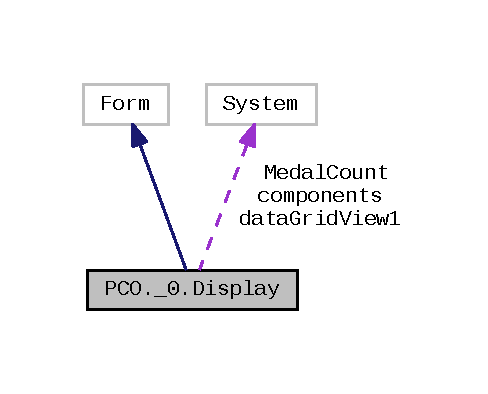
\includegraphics[width=234pt]{classPCO_1_1__0_1_1Display__coll__graph}
\end{center}
\end{figure}
\subsection*{Public Member Functions}
\begin{DoxyCompactItemize}
\item 
\hyperlink{classPCO_1_1__0_1_1Display_a4f14e8f662deb892a2c07dc78da701dc}{Display} ()
\end{DoxyCompactItemize}
\subsection*{Protected Member Functions}
\begin{DoxyCompactItemize}
\item 
override void \hyperlink{classPCO_1_1__0_1_1Display_aeec182b8e0272728a07deb3245fb3ef2}{Dispose} (bool disposing)
\begin{DoxyCompactList}\small\item\em Clean up any resources being used. \end{DoxyCompactList}\end{DoxyCompactItemize}
\subsection*{Private Member Functions}
\begin{DoxyCompactItemize}
\item 
void \hyperlink{classPCO_1_1__0_1_1Display_aa37caaa188d791b95b8d79dc1bbc953e}{Form6\+\_\+\+Load} (object sender, Event\+Args e)
\item 
void \hyperlink{classPCO_1_1__0_1_1Display_a79a83d7954cbce514cdaa8336a5af2b8}{list\+Box1\+\_\+\+Selected\+Index\+Changed} (object sender, Event\+Args e)
\item 
void \hyperlink{classPCO_1_1__0_1_1Display_a4c56052f9f51cbdff10fcb1a4d55f750}{Initialize\+Component} ()
\begin{DoxyCompactList}\small\item\em Required method for Designer support -\/ do not modify the contents of this method with the code editor. \end{DoxyCompactList}\end{DoxyCompactItemize}
\subsection*{Private Attributes}
\begin{DoxyCompactItemize}
\item 
System.\+Component\+Model.\+I\+Container \hyperlink{classPCO_1_1__0_1_1Display_a85da09902d8b1e0f454a66ad815d6090}{components} = null
\begin{DoxyCompactList}\small\item\em Required designer variable. \end{DoxyCompactList}\item 
System.\+Windows.\+Forms.\+Data\+Grid\+View \hyperlink{classPCO_1_1__0_1_1Display_a6ce931b1d769166bae50e36dd725f25b}{data\+Grid\+View1}
\item 
System.\+Windows.\+Forms.\+Data\+Grid\+View\+Text\+Box\+Column \hyperlink{classPCO_1_1__0_1_1Display_adce8cb6a82a4b034fe3b85f2192a0176}{Medal\+Count}
\end{DoxyCompactItemize}


\subsection{Detailed Description}
\hyperlink{classPCO_1_1__0_1_1Display}{Display} class for G\+UI. 

\begin{DoxyAuthor}{Author}
Landen Marchand 
\end{DoxyAuthor}


Definition at line 17 of file Display.\+cs.



\subsection{Constructor \& Destructor Documentation}
\mbox{\Hypertarget{classPCO_1_1__0_1_1Display_a4f14e8f662deb892a2c07dc78da701dc}\label{classPCO_1_1__0_1_1Display_a4f14e8f662deb892a2c07dc78da701dc}} 
\index{P\+C\+O\+::\+\_\+0\+::\+Display@{P\+C\+O\+::\+\_\+0\+::\+Display}!Display@{Display}}
\index{Display@{Display}!P\+C\+O\+::\+\_\+0\+::\+Display@{P\+C\+O\+::\+\_\+0\+::\+Display}}
\subsubsection{\texorpdfstring{Display()}{Display()}}
{\footnotesize\ttfamily P\+C\+O.\+\_\+0.\+Display.\+Display (\begin{DoxyParamCaption}{ }\end{DoxyParamCaption})\hspace{0.3cm}{\ttfamily [inline]}}



Definition at line 19 of file Display.\+cs.



\subsection{Member Function Documentation}
\mbox{\Hypertarget{classPCO_1_1__0_1_1Display_aeec182b8e0272728a07deb3245fb3ef2}\label{classPCO_1_1__0_1_1Display_aeec182b8e0272728a07deb3245fb3ef2}} 
\index{P\+C\+O\+::\+\_\+0\+::\+Display@{P\+C\+O\+::\+\_\+0\+::\+Display}!Dispose@{Dispose}}
\index{Dispose@{Dispose}!P\+C\+O\+::\+\_\+0\+::\+Display@{P\+C\+O\+::\+\_\+0\+::\+Display}}
\subsubsection{\texorpdfstring{Dispose()}{Dispose()}}
{\footnotesize\ttfamily override void P\+C\+O.\+\_\+0.\+Display.\+Dispose (\begin{DoxyParamCaption}\item[{bool}]{disposing }\end{DoxyParamCaption})\hspace{0.3cm}{\ttfamily [inline]}, {\ttfamily [protected]}}



Clean up any resources being used. 


\begin{DoxyParams}{Parameters}
{\em disposing} & true if managed resources should be disposed; otherwise, false.\\
\hline
\end{DoxyParams}


Definition at line 14 of file Display.\+Designer.\+cs.

\mbox{\Hypertarget{classPCO_1_1__0_1_1Display_aa37caaa188d791b95b8d79dc1bbc953e}\label{classPCO_1_1__0_1_1Display_aa37caaa188d791b95b8d79dc1bbc953e}} 
\index{P\+C\+O\+::\+\_\+0\+::\+Display@{P\+C\+O\+::\+\_\+0\+::\+Display}!Form6\+\_\+\+Load@{Form6\+\_\+\+Load}}
\index{Form6\+\_\+\+Load@{Form6\+\_\+\+Load}!P\+C\+O\+::\+\_\+0\+::\+Display@{P\+C\+O\+::\+\_\+0\+::\+Display}}
\subsubsection{\texorpdfstring{Form6\+\_\+\+Load()}{Form6\_Load()}}
{\footnotesize\ttfamily void P\+C\+O.\+\_\+0.\+Display.\+Form6\+\_\+\+Load (\begin{DoxyParamCaption}\item[{object}]{sender,  }\item[{Event\+Args}]{e }\end{DoxyParamCaption})\hspace{0.3cm}{\ttfamily [inline]}, {\ttfamily [private]}}



Definition at line 24 of file Display.\+cs.

\mbox{\Hypertarget{classPCO_1_1__0_1_1Display_a4c56052f9f51cbdff10fcb1a4d55f750}\label{classPCO_1_1__0_1_1Display_a4c56052f9f51cbdff10fcb1a4d55f750}} 
\index{P\+C\+O\+::\+\_\+0\+::\+Display@{P\+C\+O\+::\+\_\+0\+::\+Display}!Initialize\+Component@{Initialize\+Component}}
\index{Initialize\+Component@{Initialize\+Component}!P\+C\+O\+::\+\_\+0\+::\+Display@{P\+C\+O\+::\+\_\+0\+::\+Display}}
\subsubsection{\texorpdfstring{Initialize\+Component()}{InitializeComponent()}}
{\footnotesize\ttfamily void P\+C\+O.\+\_\+0.\+Display.\+Initialize\+Component (\begin{DoxyParamCaption}{ }\end{DoxyParamCaption})\hspace{0.3cm}{\ttfamily [inline]}, {\ttfamily [private]}}



Required method for Designer support -\/ do not modify the contents of this method with the code editor. 



Definition at line 29 of file Display.\+Designer.\+cs.

\mbox{\Hypertarget{classPCO_1_1__0_1_1Display_a79a83d7954cbce514cdaa8336a5af2b8}\label{classPCO_1_1__0_1_1Display_a79a83d7954cbce514cdaa8336a5af2b8}} 
\index{P\+C\+O\+::\+\_\+0\+::\+Display@{P\+C\+O\+::\+\_\+0\+::\+Display}!list\+Box1\+\_\+\+Selected\+Index\+Changed@{list\+Box1\+\_\+\+Selected\+Index\+Changed}}
\index{list\+Box1\+\_\+\+Selected\+Index\+Changed@{list\+Box1\+\_\+\+Selected\+Index\+Changed}!P\+C\+O\+::\+\_\+0\+::\+Display@{P\+C\+O\+::\+\_\+0\+::\+Display}}
\subsubsection{\texorpdfstring{list\+Box1\+\_\+\+Selected\+Index\+Changed()}{listBox1\_SelectedIndexChanged()}}
{\footnotesize\ttfamily void P\+C\+O.\+\_\+0.\+Display.\+list\+Box1\+\_\+\+Selected\+Index\+Changed (\begin{DoxyParamCaption}\item[{object}]{sender,  }\item[{Event\+Args}]{e }\end{DoxyParamCaption})\hspace{0.3cm}{\ttfamily [inline]}, {\ttfamily [private]}}



Definition at line 640 of file Display.\+cs.



\subsection{Member Data Documentation}
\mbox{\Hypertarget{classPCO_1_1__0_1_1Display_a85da09902d8b1e0f454a66ad815d6090}\label{classPCO_1_1__0_1_1Display_a85da09902d8b1e0f454a66ad815d6090}} 
\index{P\+C\+O\+::\+\_\+0\+::\+Display@{P\+C\+O\+::\+\_\+0\+::\+Display}!components@{components}}
\index{components@{components}!P\+C\+O\+::\+\_\+0\+::\+Display@{P\+C\+O\+::\+\_\+0\+::\+Display}}
\subsubsection{\texorpdfstring{components}{components}}
{\footnotesize\ttfamily System.\+Component\+Model.\+I\+Container P\+C\+O.\+\_\+0.\+Display.\+components = null\hspace{0.3cm}{\ttfamily [private]}}



Required designer variable. 



Definition at line 8 of file Display.\+Designer.\+cs.

\mbox{\Hypertarget{classPCO_1_1__0_1_1Display_a6ce931b1d769166bae50e36dd725f25b}\label{classPCO_1_1__0_1_1Display_a6ce931b1d769166bae50e36dd725f25b}} 
\index{P\+C\+O\+::\+\_\+0\+::\+Display@{P\+C\+O\+::\+\_\+0\+::\+Display}!data\+Grid\+View1@{data\+Grid\+View1}}
\index{data\+Grid\+View1@{data\+Grid\+View1}!P\+C\+O\+::\+\_\+0\+::\+Display@{P\+C\+O\+::\+\_\+0\+::\+Display}}
\subsubsection{\texorpdfstring{data\+Grid\+View1}{dataGridView1}}
{\footnotesize\ttfamily System.\+Windows.\+Forms.\+Data\+Grid\+View P\+C\+O.\+\_\+0.\+Display.\+data\+Grid\+View1\hspace{0.3cm}{\ttfamily [private]}}



Definition at line 69 of file Display.\+Designer.\+cs.

\mbox{\Hypertarget{classPCO_1_1__0_1_1Display_adce8cb6a82a4b034fe3b85f2192a0176}\label{classPCO_1_1__0_1_1Display_adce8cb6a82a4b034fe3b85f2192a0176}} 
\index{P\+C\+O\+::\+\_\+0\+::\+Display@{P\+C\+O\+::\+\_\+0\+::\+Display}!Medal\+Count@{Medal\+Count}}
\index{Medal\+Count@{Medal\+Count}!P\+C\+O\+::\+\_\+0\+::\+Display@{P\+C\+O\+::\+\_\+0\+::\+Display}}
\subsubsection{\texorpdfstring{Medal\+Count}{MedalCount}}
{\footnotesize\ttfamily System.\+Windows.\+Forms.\+Data\+Grid\+View\+Text\+Box\+Column P\+C\+O.\+\_\+0.\+Display.\+Medal\+Count\hspace{0.3cm}{\ttfamily [private]}}



Definition at line 70 of file Display.\+Designer.\+cs.



The documentation for this class was generated from the following files\+:\begin{DoxyCompactItemize}
\item 
\hyperlink{Display_8cs}{Display.\+cs}\item 
\hyperlink{Display_8Designer_8cs}{Display.\+Designer.\+cs}\end{DoxyCompactItemize}

\hypertarget{classPCO_1_1__0_1_1Form1}{}\section{P\+C\+O.\+\_\+0.\+Form1 Class Reference}
\label{classPCO_1_1__0_1_1Form1}\index{P\+C\+O.\+\_\+0.\+Form1@{P\+C\+O.\+\_\+0.\+Form1}}


Main Screen class for G\+UI.  




Inheritance diagram for P\+C\+O.\+\_\+0.\+Form1\+:\nopagebreak
\begin{figure}[H]
\begin{center}
\leavevmode
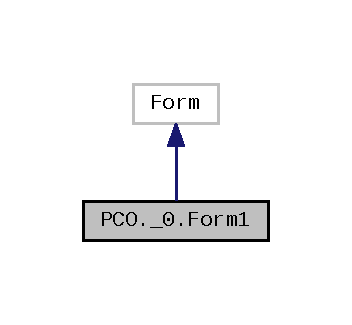
\includegraphics[width=169pt]{classPCO_1_1__0_1_1Form1__inherit__graph}
\end{center}
\end{figure}


Collaboration diagram for P\+C\+O.\+\_\+0.\+Form1\+:\nopagebreak
\begin{figure}[H]
\begin{center}
\leavevmode
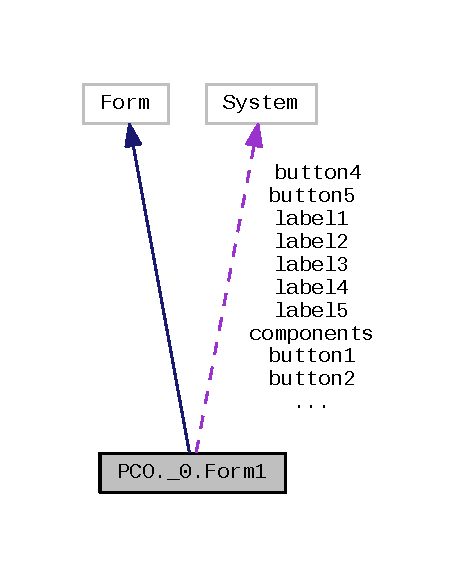
\includegraphics[width=221pt]{classPCO_1_1__0_1_1Form1__coll__graph}
\end{center}
\end{figure}
\subsection*{Public Member Functions}
\begin{DoxyCompactItemize}
\item 
\hyperlink{classPCO_1_1__0_1_1Form1_a70fd4d599a7d0db69c4ffd802816ebeb}{Form1} ()
\end{DoxyCompactItemize}
\subsection*{Protected Member Functions}
\begin{DoxyCompactItemize}
\item 
override void \hyperlink{classPCO_1_1__0_1_1Form1_ad3d7e394a984eb802f4ce2bbda31ee62}{Dispose} (bool disposing)
\begin{DoxyCompactList}\small\item\em Clean up any resources being used. \end{DoxyCompactList}\end{DoxyCompactItemize}
\subsection*{Private Member Functions}
\begin{DoxyCompactItemize}
\item 
void \hyperlink{classPCO_1_1__0_1_1Form1_ad0b73303308d064881f00e8b0f6db48c}{Form1\+\_\+\+Load} (object sender, Event\+Args e)
\item 
void \hyperlink{classPCO_1_1__0_1_1Form1_a9c714d75d45575cd760778906b458a75}{button1\+\_\+\+Click} (object sender, Event\+Args e)
\item 
void \hyperlink{classPCO_1_1__0_1_1Form1_a6324540487e979b07fb0ab76ba67e7fc}{button2\+\_\+\+Click} (object sender, Event\+Args e)
\item 
void \hyperlink{classPCO_1_1__0_1_1Form1_a6654d9632be04dacf3e2d4473f209a28}{button5\+\_\+\+Click} (object sender, Event\+Args e)
\item 
void \hyperlink{classPCO_1_1__0_1_1Form1_a1a9e0a8f7287ca33a074a1c14b358252}{button3\+\_\+\+Click} (object sender, Event\+Args e)
\item 
void \hyperlink{classPCO_1_1__0_1_1Form1_ae8703ead38c86560e75a2754a8fd2ca0}{button4\+\_\+\+Click} (object sender, Event\+Args e)
\item 
void \hyperlink{classPCO_1_1__0_1_1Form1_a27fd22008e6d99921f9e193bd4d05c14}{Initialize\+Component} ()
\begin{DoxyCompactList}\small\item\em Required method for Designer support -\/ do not modify the contents of this method with the code editor. \end{DoxyCompactList}\end{DoxyCompactItemize}
\subsection*{Private Attributes}
\begin{DoxyCompactItemize}
\item 
System.\+Component\+Model.\+I\+Container \hyperlink{classPCO_1_1__0_1_1Form1_a614991e9397c076be2839e7021dc2f52}{components} = null
\begin{DoxyCompactList}\small\item\em Required designer variable. \end{DoxyCompactList}\item 
System.\+Windows.\+Forms.\+Button \hyperlink{classPCO_1_1__0_1_1Form1_af3e0364451a4d42b57d6e88d9b228b76}{button1}
\item 
System.\+Windows.\+Forms.\+Button \hyperlink{classPCO_1_1__0_1_1Form1_a7fae69d92446bd162912641481525170}{button2}
\item 
System.\+Windows.\+Forms.\+Button \hyperlink{classPCO_1_1__0_1_1Form1_a99473f0eda59346164d688a87a891ed1}{button3}
\item 
System.\+Windows.\+Forms.\+Button \hyperlink{classPCO_1_1__0_1_1Form1_a9ec1aecf37436e397b2812daad187c79}{button4}
\item 
System.\+Windows.\+Forms.\+Label \hyperlink{classPCO_1_1__0_1_1Form1_a7e49f562daa78670a4cc691f2f2cd311}{label1}
\item 
System.\+Windows.\+Forms.\+Label \hyperlink{classPCO_1_1__0_1_1Form1_a559c2f693a93d22068d3e3cbe02f9ff2}{label2}
\item 
System.\+Windows.\+Forms.\+Label \hyperlink{classPCO_1_1__0_1_1Form1_a10a68bb406aeae6edee2ebca3f3e2795}{label3}
\item 
System.\+Windows.\+Forms.\+Label \hyperlink{classPCO_1_1__0_1_1Form1_aa13c9160937ae7c6bd69f4cb984674e1}{label4}
\item 
System.\+Windows.\+Forms.\+Label \hyperlink{classPCO_1_1__0_1_1Form1_a617d8ed5e91d6d0827eff324fcf30292}{label5}
\item 
System.\+Windows.\+Forms.\+Button \hyperlink{classPCO_1_1__0_1_1Form1_a336a0f6934f9cb5f9d3fbb050849030f}{button5}
\end{DoxyCompactItemize}


\subsection{Detailed Description}
Main Screen class for G\+UI. 

Definition at line 17 of file Form1.\+cs.



\subsection{Constructor \& Destructor Documentation}
\mbox{\Hypertarget{classPCO_1_1__0_1_1Form1_a70fd4d599a7d0db69c4ffd802816ebeb}\label{classPCO_1_1__0_1_1Form1_a70fd4d599a7d0db69c4ffd802816ebeb}} 
\index{P\+C\+O\+::\+\_\+0\+::\+Form1@{P\+C\+O\+::\+\_\+0\+::\+Form1}!Form1@{Form1}}
\index{Form1@{Form1}!P\+C\+O\+::\+\_\+0\+::\+Form1@{P\+C\+O\+::\+\_\+0\+::\+Form1}}
\subsubsection{\texorpdfstring{Form1()}{Form1()}}
{\footnotesize\ttfamily P\+C\+O.\+\_\+0.\+Form1.\+Form1 (\begin{DoxyParamCaption}{ }\end{DoxyParamCaption})\hspace{0.3cm}{\ttfamily [inline]}}



Definition at line 20 of file Form1.\+cs.



\subsection{Member Function Documentation}
\mbox{\Hypertarget{classPCO_1_1__0_1_1Form1_a9c714d75d45575cd760778906b458a75}\label{classPCO_1_1__0_1_1Form1_a9c714d75d45575cd760778906b458a75}} 
\index{P\+C\+O\+::\+\_\+0\+::\+Form1@{P\+C\+O\+::\+\_\+0\+::\+Form1}!button1\+\_\+\+Click@{button1\+\_\+\+Click}}
\index{button1\+\_\+\+Click@{button1\+\_\+\+Click}!P\+C\+O\+::\+\_\+0\+::\+Form1@{P\+C\+O\+::\+\_\+0\+::\+Form1}}
\subsubsection{\texorpdfstring{button1\+\_\+\+Click()}{button1\_Click()}}
{\footnotesize\ttfamily void P\+C\+O.\+\_\+0.\+Form1.\+button1\+\_\+\+Click (\begin{DoxyParamCaption}\item[{object}]{sender,  }\item[{Event\+Args}]{e }\end{DoxyParamCaption})\hspace{0.3cm}{\ttfamily [inline]}, {\ttfamily [private]}}



Definition at line 30 of file Form1.\+cs.

\mbox{\Hypertarget{classPCO_1_1__0_1_1Form1_a6324540487e979b07fb0ab76ba67e7fc}\label{classPCO_1_1__0_1_1Form1_a6324540487e979b07fb0ab76ba67e7fc}} 
\index{P\+C\+O\+::\+\_\+0\+::\+Form1@{P\+C\+O\+::\+\_\+0\+::\+Form1}!button2\+\_\+\+Click@{button2\+\_\+\+Click}}
\index{button2\+\_\+\+Click@{button2\+\_\+\+Click}!P\+C\+O\+::\+\_\+0\+::\+Form1@{P\+C\+O\+::\+\_\+0\+::\+Form1}}
\subsubsection{\texorpdfstring{button2\+\_\+\+Click()}{button2\_Click()}}
{\footnotesize\ttfamily void P\+C\+O.\+\_\+0.\+Form1.\+button2\+\_\+\+Click (\begin{DoxyParamCaption}\item[{object}]{sender,  }\item[{Event\+Args}]{e }\end{DoxyParamCaption})\hspace{0.3cm}{\ttfamily [inline]}, {\ttfamily [private]}}



Definition at line 36 of file Form1.\+cs.

\mbox{\Hypertarget{classPCO_1_1__0_1_1Form1_a1a9e0a8f7287ca33a074a1c14b358252}\label{classPCO_1_1__0_1_1Form1_a1a9e0a8f7287ca33a074a1c14b358252}} 
\index{P\+C\+O\+::\+\_\+0\+::\+Form1@{P\+C\+O\+::\+\_\+0\+::\+Form1}!button3\+\_\+\+Click@{button3\+\_\+\+Click}}
\index{button3\+\_\+\+Click@{button3\+\_\+\+Click}!P\+C\+O\+::\+\_\+0\+::\+Form1@{P\+C\+O\+::\+\_\+0\+::\+Form1}}
\subsubsection{\texorpdfstring{button3\+\_\+\+Click()}{button3\_Click()}}
{\footnotesize\ttfamily void P\+C\+O.\+\_\+0.\+Form1.\+button3\+\_\+\+Click (\begin{DoxyParamCaption}\item[{object}]{sender,  }\item[{Event\+Args}]{e }\end{DoxyParamCaption})\hspace{0.3cm}{\ttfamily [inline]}, {\ttfamily [private]}}



Definition at line 48 of file Form1.\+cs.

\mbox{\Hypertarget{classPCO_1_1__0_1_1Form1_ae8703ead38c86560e75a2754a8fd2ca0}\label{classPCO_1_1__0_1_1Form1_ae8703ead38c86560e75a2754a8fd2ca0}} 
\index{P\+C\+O\+::\+\_\+0\+::\+Form1@{P\+C\+O\+::\+\_\+0\+::\+Form1}!button4\+\_\+\+Click@{button4\+\_\+\+Click}}
\index{button4\+\_\+\+Click@{button4\+\_\+\+Click}!P\+C\+O\+::\+\_\+0\+::\+Form1@{P\+C\+O\+::\+\_\+0\+::\+Form1}}
\subsubsection{\texorpdfstring{button4\+\_\+\+Click()}{button4\_Click()}}
{\footnotesize\ttfamily void P\+C\+O.\+\_\+0.\+Form1.\+button4\+\_\+\+Click (\begin{DoxyParamCaption}\item[{object}]{sender,  }\item[{Event\+Args}]{e }\end{DoxyParamCaption})\hspace{0.3cm}{\ttfamily [inline]}, {\ttfamily [private]}}



Definition at line 54 of file Form1.\+cs.

\mbox{\Hypertarget{classPCO_1_1__0_1_1Form1_a6654d9632be04dacf3e2d4473f209a28}\label{classPCO_1_1__0_1_1Form1_a6654d9632be04dacf3e2d4473f209a28}} 
\index{P\+C\+O\+::\+\_\+0\+::\+Form1@{P\+C\+O\+::\+\_\+0\+::\+Form1}!button5\+\_\+\+Click@{button5\+\_\+\+Click}}
\index{button5\+\_\+\+Click@{button5\+\_\+\+Click}!P\+C\+O\+::\+\_\+0\+::\+Form1@{P\+C\+O\+::\+\_\+0\+::\+Form1}}
\subsubsection{\texorpdfstring{button5\+\_\+\+Click()}{button5\_Click()}}
{\footnotesize\ttfamily void P\+C\+O.\+\_\+0.\+Form1.\+button5\+\_\+\+Click (\begin{DoxyParamCaption}\item[{object}]{sender,  }\item[{Event\+Args}]{e }\end{DoxyParamCaption})\hspace{0.3cm}{\ttfamily [inline]}, {\ttfamily [private]}}



Definition at line 42 of file Form1.\+cs.

\mbox{\Hypertarget{classPCO_1_1__0_1_1Form1_ad3d7e394a984eb802f4ce2bbda31ee62}\label{classPCO_1_1__0_1_1Form1_ad3d7e394a984eb802f4ce2bbda31ee62}} 
\index{P\+C\+O\+::\+\_\+0\+::\+Form1@{P\+C\+O\+::\+\_\+0\+::\+Form1}!Dispose@{Dispose}}
\index{Dispose@{Dispose}!P\+C\+O\+::\+\_\+0\+::\+Form1@{P\+C\+O\+::\+\_\+0\+::\+Form1}}
\subsubsection{\texorpdfstring{Dispose()}{Dispose()}}
{\footnotesize\ttfamily override void P\+C\+O.\+\_\+0.\+Form1.\+Dispose (\begin{DoxyParamCaption}\item[{bool}]{disposing }\end{DoxyParamCaption})\hspace{0.3cm}{\ttfamily [inline]}, {\ttfamily [protected]}}



Clean up any resources being used. 


\begin{DoxyParams}{Parameters}
{\em disposing} & true if managed resources should be disposed; otherwise, false.\\
\hline
\end{DoxyParams}


Definition at line 14 of file Form1.\+Designer.\+cs.

\mbox{\Hypertarget{classPCO_1_1__0_1_1Form1_ad0b73303308d064881f00e8b0f6db48c}\label{classPCO_1_1__0_1_1Form1_ad0b73303308d064881f00e8b0f6db48c}} 
\index{P\+C\+O\+::\+\_\+0\+::\+Form1@{P\+C\+O\+::\+\_\+0\+::\+Form1}!Form1\+\_\+\+Load@{Form1\+\_\+\+Load}}
\index{Form1\+\_\+\+Load@{Form1\+\_\+\+Load}!P\+C\+O\+::\+\_\+0\+::\+Form1@{P\+C\+O\+::\+\_\+0\+::\+Form1}}
\subsubsection{\texorpdfstring{Form1\+\_\+\+Load()}{Form1\_Load()}}
{\footnotesize\ttfamily void P\+C\+O.\+\_\+0.\+Form1.\+Form1\+\_\+\+Load (\begin{DoxyParamCaption}\item[{object}]{sender,  }\item[{Event\+Args}]{e }\end{DoxyParamCaption})\hspace{0.3cm}{\ttfamily [inline]}, {\ttfamily [private]}}



Definition at line 25 of file Form1.\+cs.

\mbox{\Hypertarget{classPCO_1_1__0_1_1Form1_a27fd22008e6d99921f9e193bd4d05c14}\label{classPCO_1_1__0_1_1Form1_a27fd22008e6d99921f9e193bd4d05c14}} 
\index{P\+C\+O\+::\+\_\+0\+::\+Form1@{P\+C\+O\+::\+\_\+0\+::\+Form1}!Initialize\+Component@{Initialize\+Component}}
\index{Initialize\+Component@{Initialize\+Component}!P\+C\+O\+::\+\_\+0\+::\+Form1@{P\+C\+O\+::\+\_\+0\+::\+Form1}}
\subsubsection{\texorpdfstring{Initialize\+Component()}{InitializeComponent()}}
{\footnotesize\ttfamily void P\+C\+O.\+\_\+0.\+Form1.\+Initialize\+Component (\begin{DoxyParamCaption}{ }\end{DoxyParamCaption})\hspace{0.3cm}{\ttfamily [inline]}, {\ttfamily [private]}}



Required method for Designer support -\/ do not modify the contents of this method with the code editor. 



Definition at line 29 of file Form1.\+Designer.\+cs.



\subsection{Member Data Documentation}
\mbox{\Hypertarget{classPCO_1_1__0_1_1Form1_af3e0364451a4d42b57d6e88d9b228b76}\label{classPCO_1_1__0_1_1Form1_af3e0364451a4d42b57d6e88d9b228b76}} 
\index{P\+C\+O\+::\+\_\+0\+::\+Form1@{P\+C\+O\+::\+\_\+0\+::\+Form1}!button1@{button1}}
\index{button1@{button1}!P\+C\+O\+::\+\_\+0\+::\+Form1@{P\+C\+O\+::\+\_\+0\+::\+Form1}}
\subsubsection{\texorpdfstring{button1}{button1}}
{\footnotesize\ttfamily System.\+Windows.\+Forms.\+Button P\+C\+O.\+\_\+0.\+Form1.\+button1\hspace{0.3cm}{\ttfamily [private]}}



Definition at line 165 of file Form1.\+Designer.\+cs.

\mbox{\Hypertarget{classPCO_1_1__0_1_1Form1_a7fae69d92446bd162912641481525170}\label{classPCO_1_1__0_1_1Form1_a7fae69d92446bd162912641481525170}} 
\index{P\+C\+O\+::\+\_\+0\+::\+Form1@{P\+C\+O\+::\+\_\+0\+::\+Form1}!button2@{button2}}
\index{button2@{button2}!P\+C\+O\+::\+\_\+0\+::\+Form1@{P\+C\+O\+::\+\_\+0\+::\+Form1}}
\subsubsection{\texorpdfstring{button2}{button2}}
{\footnotesize\ttfamily System.\+Windows.\+Forms.\+Button P\+C\+O.\+\_\+0.\+Form1.\+button2\hspace{0.3cm}{\ttfamily [private]}}



Definition at line 166 of file Form1.\+Designer.\+cs.

\mbox{\Hypertarget{classPCO_1_1__0_1_1Form1_a99473f0eda59346164d688a87a891ed1}\label{classPCO_1_1__0_1_1Form1_a99473f0eda59346164d688a87a891ed1}} 
\index{P\+C\+O\+::\+\_\+0\+::\+Form1@{P\+C\+O\+::\+\_\+0\+::\+Form1}!button3@{button3}}
\index{button3@{button3}!P\+C\+O\+::\+\_\+0\+::\+Form1@{P\+C\+O\+::\+\_\+0\+::\+Form1}}
\subsubsection{\texorpdfstring{button3}{button3}}
{\footnotesize\ttfamily System.\+Windows.\+Forms.\+Button P\+C\+O.\+\_\+0.\+Form1.\+button3\hspace{0.3cm}{\ttfamily [private]}}



Definition at line 167 of file Form1.\+Designer.\+cs.

\mbox{\Hypertarget{classPCO_1_1__0_1_1Form1_a9ec1aecf37436e397b2812daad187c79}\label{classPCO_1_1__0_1_1Form1_a9ec1aecf37436e397b2812daad187c79}} 
\index{P\+C\+O\+::\+\_\+0\+::\+Form1@{P\+C\+O\+::\+\_\+0\+::\+Form1}!button4@{button4}}
\index{button4@{button4}!P\+C\+O\+::\+\_\+0\+::\+Form1@{P\+C\+O\+::\+\_\+0\+::\+Form1}}
\subsubsection{\texorpdfstring{button4}{button4}}
{\footnotesize\ttfamily System.\+Windows.\+Forms.\+Button P\+C\+O.\+\_\+0.\+Form1.\+button4\hspace{0.3cm}{\ttfamily [private]}}



Definition at line 168 of file Form1.\+Designer.\+cs.

\mbox{\Hypertarget{classPCO_1_1__0_1_1Form1_a336a0f6934f9cb5f9d3fbb050849030f}\label{classPCO_1_1__0_1_1Form1_a336a0f6934f9cb5f9d3fbb050849030f}} 
\index{P\+C\+O\+::\+\_\+0\+::\+Form1@{P\+C\+O\+::\+\_\+0\+::\+Form1}!button5@{button5}}
\index{button5@{button5}!P\+C\+O\+::\+\_\+0\+::\+Form1@{P\+C\+O\+::\+\_\+0\+::\+Form1}}
\subsubsection{\texorpdfstring{button5}{button5}}
{\footnotesize\ttfamily System.\+Windows.\+Forms.\+Button P\+C\+O.\+\_\+0.\+Form1.\+button5\hspace{0.3cm}{\ttfamily [private]}}



Definition at line 174 of file Form1.\+Designer.\+cs.

\mbox{\Hypertarget{classPCO_1_1__0_1_1Form1_a614991e9397c076be2839e7021dc2f52}\label{classPCO_1_1__0_1_1Form1_a614991e9397c076be2839e7021dc2f52}} 
\index{P\+C\+O\+::\+\_\+0\+::\+Form1@{P\+C\+O\+::\+\_\+0\+::\+Form1}!components@{components}}
\index{components@{components}!P\+C\+O\+::\+\_\+0\+::\+Form1@{P\+C\+O\+::\+\_\+0\+::\+Form1}}
\subsubsection{\texorpdfstring{components}{components}}
{\footnotesize\ttfamily System.\+Component\+Model.\+I\+Container P\+C\+O.\+\_\+0.\+Form1.\+components = null\hspace{0.3cm}{\ttfamily [private]}}



Required designer variable. 



Definition at line 8 of file Form1.\+Designer.\+cs.

\mbox{\Hypertarget{classPCO_1_1__0_1_1Form1_a7e49f562daa78670a4cc691f2f2cd311}\label{classPCO_1_1__0_1_1Form1_a7e49f562daa78670a4cc691f2f2cd311}} 
\index{P\+C\+O\+::\+\_\+0\+::\+Form1@{P\+C\+O\+::\+\_\+0\+::\+Form1}!label1@{label1}}
\index{label1@{label1}!P\+C\+O\+::\+\_\+0\+::\+Form1@{P\+C\+O\+::\+\_\+0\+::\+Form1}}
\subsubsection{\texorpdfstring{label1}{label1}}
{\footnotesize\ttfamily System.\+Windows.\+Forms.\+Label P\+C\+O.\+\_\+0.\+Form1.\+label1\hspace{0.3cm}{\ttfamily [private]}}



Definition at line 169 of file Form1.\+Designer.\+cs.

\mbox{\Hypertarget{classPCO_1_1__0_1_1Form1_a559c2f693a93d22068d3e3cbe02f9ff2}\label{classPCO_1_1__0_1_1Form1_a559c2f693a93d22068d3e3cbe02f9ff2}} 
\index{P\+C\+O\+::\+\_\+0\+::\+Form1@{P\+C\+O\+::\+\_\+0\+::\+Form1}!label2@{label2}}
\index{label2@{label2}!P\+C\+O\+::\+\_\+0\+::\+Form1@{P\+C\+O\+::\+\_\+0\+::\+Form1}}
\subsubsection{\texorpdfstring{label2}{label2}}
{\footnotesize\ttfamily System.\+Windows.\+Forms.\+Label P\+C\+O.\+\_\+0.\+Form1.\+label2\hspace{0.3cm}{\ttfamily [private]}}



Definition at line 170 of file Form1.\+Designer.\+cs.

\mbox{\Hypertarget{classPCO_1_1__0_1_1Form1_a10a68bb406aeae6edee2ebca3f3e2795}\label{classPCO_1_1__0_1_1Form1_a10a68bb406aeae6edee2ebca3f3e2795}} 
\index{P\+C\+O\+::\+\_\+0\+::\+Form1@{P\+C\+O\+::\+\_\+0\+::\+Form1}!label3@{label3}}
\index{label3@{label3}!P\+C\+O\+::\+\_\+0\+::\+Form1@{P\+C\+O\+::\+\_\+0\+::\+Form1}}
\subsubsection{\texorpdfstring{label3}{label3}}
{\footnotesize\ttfamily System.\+Windows.\+Forms.\+Label P\+C\+O.\+\_\+0.\+Form1.\+label3\hspace{0.3cm}{\ttfamily [private]}}



Definition at line 171 of file Form1.\+Designer.\+cs.

\mbox{\Hypertarget{classPCO_1_1__0_1_1Form1_aa13c9160937ae7c6bd69f4cb984674e1}\label{classPCO_1_1__0_1_1Form1_aa13c9160937ae7c6bd69f4cb984674e1}} 
\index{P\+C\+O\+::\+\_\+0\+::\+Form1@{P\+C\+O\+::\+\_\+0\+::\+Form1}!label4@{label4}}
\index{label4@{label4}!P\+C\+O\+::\+\_\+0\+::\+Form1@{P\+C\+O\+::\+\_\+0\+::\+Form1}}
\subsubsection{\texorpdfstring{label4}{label4}}
{\footnotesize\ttfamily System.\+Windows.\+Forms.\+Label P\+C\+O.\+\_\+0.\+Form1.\+label4\hspace{0.3cm}{\ttfamily [private]}}



Definition at line 172 of file Form1.\+Designer.\+cs.

\mbox{\Hypertarget{classPCO_1_1__0_1_1Form1_a617d8ed5e91d6d0827eff324fcf30292}\label{classPCO_1_1__0_1_1Form1_a617d8ed5e91d6d0827eff324fcf30292}} 
\index{P\+C\+O\+::\+\_\+0\+::\+Form1@{P\+C\+O\+::\+\_\+0\+::\+Form1}!label5@{label5}}
\index{label5@{label5}!P\+C\+O\+::\+\_\+0\+::\+Form1@{P\+C\+O\+::\+\_\+0\+::\+Form1}}
\subsubsection{\texorpdfstring{label5}{label5}}
{\footnotesize\ttfamily System.\+Windows.\+Forms.\+Label P\+C\+O.\+\_\+0.\+Form1.\+label5\hspace{0.3cm}{\ttfamily [private]}}



Definition at line 173 of file Form1.\+Designer.\+cs.



The documentation for this class was generated from the following files\+:\begin{DoxyCompactItemize}
\item 
\hyperlink{Form1_8cs}{Form1.\+cs}\item 
\hyperlink{Form1_8Designer_8cs}{Form1.\+Designer.\+cs}\end{DoxyCompactItemize}

\hypertarget{classIceDance}{}\section{Ice\+Dance Class Reference}
\label{classIceDance}\index{Ice\+Dance@{Ice\+Dance}}


\hyperlink{classIceDance}{Ice\+Dance} class is one of the 3 Figure\+Skating events.  


\subsection*{Public Member Functions}
\begin{DoxyCompactItemize}
\item 
\hyperlink{classIceDance_a237069675d6d3af0a9e781d2ae34ebfe}{Ice\+Dance} ()
\item 
void \hyperlink{classIceDance_abaf4f53da183e1bee83a6e2976ce5c95}{Add\+Athlete\+Male} (string country, string Fname, string Lname)
\item 
void \hyperlink{classIceDance_a7b0f52e81042ff7cb39fc8fb3c7e6a13}{Add\+Athlete\+Female} (string country, string Fname, string Lname)
\end{DoxyCompactItemize}


\subsection{Detailed Description}
\hyperlink{classIceDance}{Ice\+Dance} class is one of the 3 Figure\+Skating events. 

D\+E\+F\+I\+N\+I\+T\+I\+ON\+: Form of figure skating where athletes participate in male/female pairs. The utilization of the same technique as Pair Skating is present but the dancing is all done in tandem versus implementing technical tricks.

C\+O\+N\+S\+T\+R\+A\+I\+N\+TS\+: The pairs are male/female. Each pair performs solo on the rink at a given time. Total duration of performance is 4 mintues and 30 seconds.\begin{DoxyAuthor}{Author}
Landen Marchand 
\end{DoxyAuthor}


Definition at line 76 of file Class1.\+cs.



\subsection{Constructor \& Destructor Documentation}
\mbox{\Hypertarget{classIceDance_a237069675d6d3af0a9e781d2ae34ebfe}\label{classIceDance_a237069675d6d3af0a9e781d2ae34ebfe}} 
\index{Ice\+Dance@{Ice\+Dance}!Ice\+Dance@{Ice\+Dance}}
\index{Ice\+Dance@{Ice\+Dance}!Ice\+Dance@{Ice\+Dance}}
\subsubsection{\texorpdfstring{Ice\+Dance()}{IceDance()}}
{\footnotesize\ttfamily Ice\+Dance.\+Ice\+Dance (\begin{DoxyParamCaption}{ }\end{DoxyParamCaption})\hspace{0.3cm}{\ttfamily [inline]}}

Default Constructor Provided Automatically 
\begin{DoxyParams}{Parameters}
{\em None} & \\
\hline
\end{DoxyParams}
\begin{DoxyReturn}{Returns}
Default Values 
\end{DoxyReturn}


Definition at line 82 of file Class1.\+cs.



\subsection{Member Function Documentation}
\mbox{\Hypertarget{classIceDance_a7b0f52e81042ff7cb39fc8fb3c7e6a13}\label{classIceDance_a7b0f52e81042ff7cb39fc8fb3c7e6a13}} 
\index{Ice\+Dance@{Ice\+Dance}!Add\+Athlete\+Female@{Add\+Athlete\+Female}}
\index{Add\+Athlete\+Female@{Add\+Athlete\+Female}!Ice\+Dance@{Ice\+Dance}}
\subsubsection{\texorpdfstring{Add\+Athlete\+Female()}{AddAthleteFemale()}}
{\footnotesize\ttfamily void Ice\+Dance.\+Add\+Athlete\+Female (\begin{DoxyParamCaption}\item[{string}]{country,  }\item[{string}]{Fname,  }\item[{string}]{Lname }\end{DoxyParamCaption})\hspace{0.3cm}{\ttfamily [inline]}}

Void function adds female to database for the event 
\begin{DoxyParams}{Parameters}
{\em string} & for athlete\textquotesingle{}s team name \\
\hline
{\em string} & for first name of athlete \\
\hline
{\em string} & for last name of athlete \\
\hline
\end{DoxyParams}
$<$ Creates variable for connection string

$<$ Opens DB Checks connection and fills grid view with Race table

$<$ Adds entry to athlete information

$<$ Opens DB Checks connection and fills grid view with Race table

$<$ Adds entry to athlete information 

Definition at line 147 of file Class1.\+cs.

\mbox{\Hypertarget{classIceDance_abaf4f53da183e1bee83a6e2976ce5c95}\label{classIceDance_abaf4f53da183e1bee83a6e2976ce5c95}} 
\index{Ice\+Dance@{Ice\+Dance}!Add\+Athlete\+Male@{Add\+Athlete\+Male}}
\index{Add\+Athlete\+Male@{Add\+Athlete\+Male}!Ice\+Dance@{Ice\+Dance}}
\subsubsection{\texorpdfstring{Add\+Athlete\+Male()}{AddAthleteMale()}}
{\footnotesize\ttfamily void Ice\+Dance.\+Add\+Athlete\+Male (\begin{DoxyParamCaption}\item[{string}]{country,  }\item[{string}]{Fname,  }\item[{string}]{Lname }\end{DoxyParamCaption})\hspace{0.3cm}{\ttfamily [inline]}}

Void function adds male to database for the event 
\begin{DoxyParams}{Parameters}
{\em string} & for athlete\textquotesingle{}s team name \\
\hline
{\em string} & for first name of athlete \\
\hline
{\em string} & for last name of athlete \\
\hline
\end{DoxyParams}
$<$ Creates variable for connection string

$<$ Opens DB Checks connection and fills grid view with Race table

$<$ Adds entry to athlete information

$<$ Opens DB Checks connection and fills grid view with Race table

$<$ Adds entry to athlete information 

Definition at line 90 of file Class1.\+cs.



The documentation for this class was generated from the following file\+:\begin{DoxyCompactItemize}
\item 
\hyperlink{Class1_8cs}{Class1.\+cs}\end{DoxyCompactItemize}

\hypertarget{classPairSkating}{}\section{Pair\+Skating Class Reference}
\label{classPairSkating}\index{Pair\+Skating@{Pair\+Skating}}


\hyperlink{classPairSkating}{Pair\+Skating} class is one of the 3 Figure\+Skating events.  


\subsection*{Public Member Functions}
\begin{DoxyCompactItemize}
\item 
void \hyperlink{classPairSkating_a32f1d4f6c99becbf394822d0abf2d508}{Add\+Athlete} (string country, string Fname, string Lname)
\end{DoxyCompactItemize}


\subsection{Detailed Description}
\hyperlink{classPairSkating}{Pair\+Skating} class is one of the 3 Figure\+Skating events. 

D\+E\+F\+I\+N\+I\+T\+I\+ON\+: Form of figure skating where athletes participate individually. The utilization of long program style where each athlete is free to do their own unique performance complete with technical tricks is present.

C\+O\+N\+S\+T\+R\+A\+I\+N\+TS\+: Each athlete performs solo on the rink at a given time. Total duration of performance is 4 minutes and 30 seconds.\begin{DoxyAuthor}{Author}
Landen Marchand 
\end{DoxyAuthor}


Definition at line 914 of file Class1.\+cs.



\subsection{Member Function Documentation}
\mbox{\Hypertarget{classPairSkating_a32f1d4f6c99becbf394822d0abf2d508}\label{classPairSkating_a32f1d4f6c99becbf394822d0abf2d508}} 
\index{Pair\+Skating@{Pair\+Skating}!Add\+Athlete@{Add\+Athlete}}
\index{Add\+Athlete@{Add\+Athlete}!Pair\+Skating@{Pair\+Skating}}
\subsubsection{\texorpdfstring{Add\+Athlete()}{AddAthlete()}}
{\footnotesize\ttfamily void Pair\+Skating.\+Add\+Athlete (\begin{DoxyParamCaption}\item[{string}]{country,  }\item[{string}]{Fname,  }\item[{string}]{Lname }\end{DoxyParamCaption})\hspace{0.3cm}{\ttfamily [inline]}}

Void function adds an athlete to database for the event 
\begin{DoxyParams}{Parameters}
{\em string} & for athlete\textquotesingle{}s team name \\
\hline
{\em string} & for first name of athlete \\
\hline
{\em string} & for last name of athlete \\
\hline
\end{DoxyParams}
$<$ Creates variable for connection string

$<$ Opens DB Checks connection and fills grid view with Race table

$<$ Adds entry to athlete information

$<$ Opens DB Checks connection and fills grid view with Race table

$<$ Adds entry to athlete information 

Definition at line 921 of file Class1.\+cs.



The documentation for this class was generated from the following file\+:\begin{DoxyCompactItemize}
\item 
\hyperlink{Class1_8cs}{Class1.\+cs}\end{DoxyCompactItemize}

\hypertarget{classPCO_1_1__0_1_1RegisterEventForm}{}\section{P\+C\+O.\+\_\+0.\+Register\+Event\+Form Class Reference}
\label{classPCO_1_1__0_1_1RegisterEventForm}\index{P\+C\+O.\+\_\+0.\+Register\+Event\+Form@{P\+C\+O.\+\_\+0.\+Register\+Event\+Form}}


Register Event class for G\+UI.  




Inheritance diagram for P\+C\+O.\+\_\+0.\+Register\+Event\+Form\+:\nopagebreak
\begin{figure}[H]
\begin{center}
\leavevmode
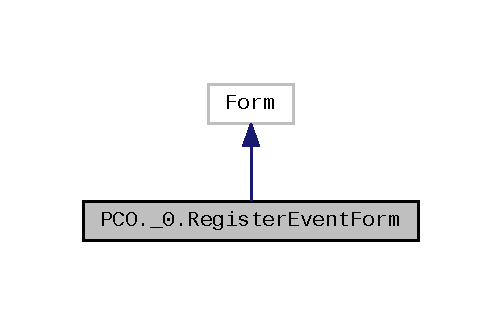
\includegraphics[width=241pt]{classPCO_1_1__0_1_1RegisterEventForm__inherit__graph}
\end{center}
\end{figure}


Collaboration diagram for P\+C\+O.\+\_\+0.\+Register\+Event\+Form\+:\nopagebreak
\begin{figure}[H]
\begin{center}
\leavevmode
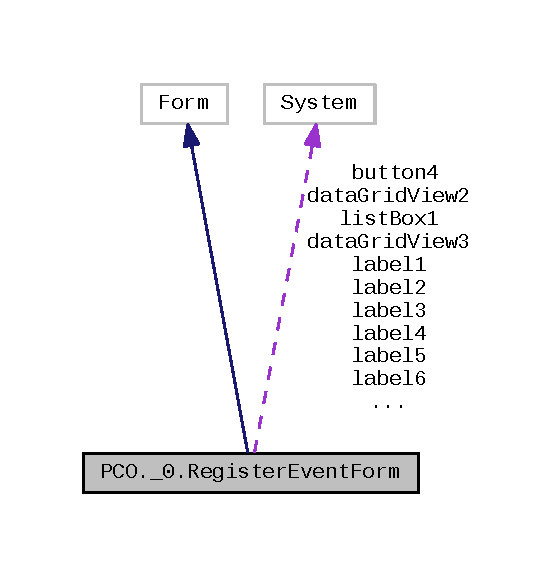
\includegraphics[width=267pt]{classPCO_1_1__0_1_1RegisterEventForm__coll__graph}
\end{center}
\end{figure}
\subsection*{Public Member Functions}
\begin{DoxyCompactItemize}
\item 
\hyperlink{classPCO_1_1__0_1_1RegisterEventForm_ad07130f7efb6992bcbf2985aa47c03f7}{Register\+Event\+Form} ()
\end{DoxyCompactItemize}
\subsection*{Protected Member Functions}
\begin{DoxyCompactItemize}
\item 
override void \hyperlink{classPCO_1_1__0_1_1RegisterEventForm_a0ae9bae95772a971a0a1965e912d1570}{Dispose} (bool disposing)
\begin{DoxyCompactList}\small\item\em Clean up any resources being used. \end{DoxyCompactList}\end{DoxyCompactItemize}
\subsection*{Private Member Functions}
\begin{DoxyCompactItemize}
\item 
void \hyperlink{classPCO_1_1__0_1_1RegisterEventForm_aae3e83a77c3537a8adb5b44bce257941}{Register\+Event\+Form\+\_\+\+Load} (object sender, Event\+Args e)
\item 
void \hyperlink{classPCO_1_1__0_1_1RegisterEventForm_a70763d4e3b7bff428a1465a3a71be63e}{button1\+\_\+\+Click} (object sender, Event\+Args e)
\item 
void \hyperlink{classPCO_1_1__0_1_1RegisterEventForm_a9d96ca1066a03fde9504b3b526bec3c9}{button3\+\_\+\+Click} (object sender, Event\+Args e)
\item 
void \hyperlink{classPCO_1_1__0_1_1RegisterEventForm_a1f2a9979dc0f8c7268fc03f9886c7a2a}{list\+Box1\+\_\+\+Selected\+Index\+Changed} (object sender, Event\+Args e)
\item 
void \hyperlink{classPCO_1_1__0_1_1RegisterEventForm_abbd7cfbf7df74e7c257c370eff4bd3f8}{button2\+\_\+\+Click} (object sender, Event\+Args e)
\item 
void \hyperlink{classPCO_1_1__0_1_1RegisterEventForm_acbfb155a6a0a01796531fee016790c9a}{button4\+\_\+\+Click} (object sender, Event\+Args e)
\item 
void \hyperlink{classPCO_1_1__0_1_1RegisterEventForm_a86205dc5856bd764865a4ee455f0aae9}{Initialize\+Component} ()
\begin{DoxyCompactList}\small\item\em Required method for Designer support -\/ do not modify the contents of this method with the code editor. \end{DoxyCompactList}\end{DoxyCompactItemize}
\subsection*{Private Attributes}
\begin{DoxyCompactItemize}
\item 
System.\+Component\+Model.\+I\+Container \hyperlink{classPCO_1_1__0_1_1RegisterEventForm_a74923b3f8c64b3221e31005393942d4b}{components} = null
\begin{DoxyCompactList}\small\item\em Required designer variable. \end{DoxyCompactList}\item 
System.\+Windows.\+Forms.\+Button \hyperlink{classPCO_1_1__0_1_1RegisterEventForm_ad03ef1b81269d53e21cd908c97a4ba88}{button1}
\item 
System.\+Windows.\+Forms.\+Data\+Grid\+View \hyperlink{classPCO_1_1__0_1_1RegisterEventForm_ae7e8ab321760d7d8e5576c2fb4997c67}{data\+Grid\+View1}
\item 
System.\+Windows.\+Forms.\+Label \hyperlink{classPCO_1_1__0_1_1RegisterEventForm_a33de43a0ef115a2e496be92676029fb7}{label1}
\item 
System.\+Windows.\+Forms.\+List\+Box \hyperlink{classPCO_1_1__0_1_1RegisterEventForm_abb9877d3121bf3c5e7fb0e63d63c4880}{list\+Box1}
\item 
System.\+Windows.\+Forms.\+Label \hyperlink{classPCO_1_1__0_1_1RegisterEventForm_a6b8bfafaa0944d0aa0b72a91eebb2a1b}{label2}
\item 
System.\+Windows.\+Forms.\+Label \hyperlink{classPCO_1_1__0_1_1RegisterEventForm_abe6115c6fe60e2f78832b7927c3b7c53}{label3}
\item 
System.\+Windows.\+Forms.\+Data\+Grid\+View \hyperlink{classPCO_1_1__0_1_1RegisterEventForm_ac65bdd45c05f09fe9ea063acb5f50a87}{data\+Grid\+View2}
\item 
System.\+Windows.\+Forms.\+Label \hyperlink{classPCO_1_1__0_1_1RegisterEventForm_a1c09d5156913257b2e9f20aec80003c5}{label4}
\item 
System.\+Windows.\+Forms.\+Label \hyperlink{classPCO_1_1__0_1_1RegisterEventForm_a3f48b3282180f7d832e660f2b26dcf74}{label6}
\item 
System.\+Windows.\+Forms.\+Button \hyperlink{classPCO_1_1__0_1_1RegisterEventForm_ad060b09ffb4cc57342e0c792eeb6d26f}{button3}
\item 
System.\+Windows.\+Forms.\+Data\+Grid\+View \hyperlink{classPCO_1_1__0_1_1RegisterEventForm_afa7b61b2882e2e3eed3e2bcb5bfa3757}{data\+Grid\+View3}
\item 
System.\+Windows.\+Forms.\+Label \hyperlink{classPCO_1_1__0_1_1RegisterEventForm_af2a7d9b72541685938323c22c5f195f9}{label5}
\item 
System.\+Windows.\+Forms.\+Button \hyperlink{classPCO_1_1__0_1_1RegisterEventForm_a8aafbb08d70f404ebfa79f3f450702c4}{button2}
\item 
System.\+Windows.\+Forms.\+Button \hyperlink{classPCO_1_1__0_1_1RegisterEventForm_a38296d81242a0466bcd44b7240cc5859}{button4}
\item 
System.\+Windows.\+Forms.\+Label \hyperlink{classPCO_1_1__0_1_1RegisterEventForm_a28576032dca99f0668fcdef4ff2c1c5f}{label7}
\item 
System.\+Windows.\+Forms.\+Label \hyperlink{classPCO_1_1__0_1_1RegisterEventForm_a44873bdda95c312ccae54bab65f1ee5e}{label8}
\end{DoxyCompactItemize}


\subsection{Detailed Description}
Register Event class for G\+UI. 

Definition at line 15 of file Event.\+cs.



\subsection{Constructor \& Destructor Documentation}
\mbox{\Hypertarget{classPCO_1_1__0_1_1RegisterEventForm_ad07130f7efb6992bcbf2985aa47c03f7}\label{classPCO_1_1__0_1_1RegisterEventForm_ad07130f7efb6992bcbf2985aa47c03f7}} 
\index{P\+C\+O\+::\+\_\+0\+::\+Register\+Event\+Form@{P\+C\+O\+::\+\_\+0\+::\+Register\+Event\+Form}!Register\+Event\+Form@{Register\+Event\+Form}}
\index{Register\+Event\+Form@{Register\+Event\+Form}!P\+C\+O\+::\+\_\+0\+::\+Register\+Event\+Form@{P\+C\+O\+::\+\_\+0\+::\+Register\+Event\+Form}}
\subsubsection{\texorpdfstring{Register\+Event\+Form()}{RegisterEventForm()}}
{\footnotesize\ttfamily P\+C\+O.\+\_\+0.\+Register\+Event\+Form.\+Register\+Event\+Form (\begin{DoxyParamCaption}{ }\end{DoxyParamCaption})\hspace{0.3cm}{\ttfamily [inline]}}



Definition at line 17 of file Event.\+cs.



\subsection{Member Function Documentation}
\mbox{\Hypertarget{classPCO_1_1__0_1_1RegisterEventForm_a70763d4e3b7bff428a1465a3a71be63e}\label{classPCO_1_1__0_1_1RegisterEventForm_a70763d4e3b7bff428a1465a3a71be63e}} 
\index{P\+C\+O\+::\+\_\+0\+::\+Register\+Event\+Form@{P\+C\+O\+::\+\_\+0\+::\+Register\+Event\+Form}!button1\+\_\+\+Click@{button1\+\_\+\+Click}}
\index{button1\+\_\+\+Click@{button1\+\_\+\+Click}!P\+C\+O\+::\+\_\+0\+::\+Register\+Event\+Form@{P\+C\+O\+::\+\_\+0\+::\+Register\+Event\+Form}}
\subsubsection{\texorpdfstring{button1\+\_\+\+Click()}{button1\_Click()}}
{\footnotesize\ttfamily void P\+C\+O.\+\_\+0.\+Register\+Event\+Form.\+button1\+\_\+\+Click (\begin{DoxyParamCaption}\item[{object}]{sender,  }\item[{Event\+Args}]{e }\end{DoxyParamCaption})\hspace{0.3cm}{\ttfamily [inline]}, {\ttfamily [private]}}



Definition at line 103 of file Event.\+cs.

\mbox{\Hypertarget{classPCO_1_1__0_1_1RegisterEventForm_abbd7cfbf7df74e7c257c370eff4bd3f8}\label{classPCO_1_1__0_1_1RegisterEventForm_abbd7cfbf7df74e7c257c370eff4bd3f8}} 
\index{P\+C\+O\+::\+\_\+0\+::\+Register\+Event\+Form@{P\+C\+O\+::\+\_\+0\+::\+Register\+Event\+Form}!button2\+\_\+\+Click@{button2\+\_\+\+Click}}
\index{button2\+\_\+\+Click@{button2\+\_\+\+Click}!P\+C\+O\+::\+\_\+0\+::\+Register\+Event\+Form@{P\+C\+O\+::\+\_\+0\+::\+Register\+Event\+Form}}
\subsubsection{\texorpdfstring{button2\+\_\+\+Click()}{button2\_Click()}}
{\footnotesize\ttfamily void P\+C\+O.\+\_\+0.\+Register\+Event\+Form.\+button2\+\_\+\+Click (\begin{DoxyParamCaption}\item[{object}]{sender,  }\item[{Event\+Args}]{e }\end{DoxyParamCaption})\hspace{0.3cm}{\ttfamily [inline]}, {\ttfamily [private]}}



Definition at line 289 of file Event.\+cs.

\mbox{\Hypertarget{classPCO_1_1__0_1_1RegisterEventForm_a9d96ca1066a03fde9504b3b526bec3c9}\label{classPCO_1_1__0_1_1RegisterEventForm_a9d96ca1066a03fde9504b3b526bec3c9}} 
\index{P\+C\+O\+::\+\_\+0\+::\+Register\+Event\+Form@{P\+C\+O\+::\+\_\+0\+::\+Register\+Event\+Form}!button3\+\_\+\+Click@{button3\+\_\+\+Click}}
\index{button3\+\_\+\+Click@{button3\+\_\+\+Click}!P\+C\+O\+::\+\_\+0\+::\+Register\+Event\+Form@{P\+C\+O\+::\+\_\+0\+::\+Register\+Event\+Form}}
\subsubsection{\texorpdfstring{button3\+\_\+\+Click()}{button3\_Click()}}
{\footnotesize\ttfamily void P\+C\+O.\+\_\+0.\+Register\+Event\+Form.\+button3\+\_\+\+Click (\begin{DoxyParamCaption}\item[{object}]{sender,  }\item[{Event\+Args}]{e }\end{DoxyParamCaption})\hspace{0.3cm}{\ttfamily [inline]}, {\ttfamily [private]}}



Definition at line 226 of file Event.\+cs.

\mbox{\Hypertarget{classPCO_1_1__0_1_1RegisterEventForm_acbfb155a6a0a01796531fee016790c9a}\label{classPCO_1_1__0_1_1RegisterEventForm_acbfb155a6a0a01796531fee016790c9a}} 
\index{P\+C\+O\+::\+\_\+0\+::\+Register\+Event\+Form@{P\+C\+O\+::\+\_\+0\+::\+Register\+Event\+Form}!button4\+\_\+\+Click@{button4\+\_\+\+Click}}
\index{button4\+\_\+\+Click@{button4\+\_\+\+Click}!P\+C\+O\+::\+\_\+0\+::\+Register\+Event\+Form@{P\+C\+O\+::\+\_\+0\+::\+Register\+Event\+Form}}
\subsubsection{\texorpdfstring{button4\+\_\+\+Click()}{button4\_Click()}}
{\footnotesize\ttfamily void P\+C\+O.\+\_\+0.\+Register\+Event\+Form.\+button4\+\_\+\+Click (\begin{DoxyParamCaption}\item[{object}]{sender,  }\item[{Event\+Args}]{e }\end{DoxyParamCaption})\hspace{0.3cm}{\ttfamily [inline]}, {\ttfamily [private]}}



Definition at line 319 of file Event.\+cs.

\mbox{\Hypertarget{classPCO_1_1__0_1_1RegisterEventForm_a0ae9bae95772a971a0a1965e912d1570}\label{classPCO_1_1__0_1_1RegisterEventForm_a0ae9bae95772a971a0a1965e912d1570}} 
\index{P\+C\+O\+::\+\_\+0\+::\+Register\+Event\+Form@{P\+C\+O\+::\+\_\+0\+::\+Register\+Event\+Form}!Dispose@{Dispose}}
\index{Dispose@{Dispose}!P\+C\+O\+::\+\_\+0\+::\+Register\+Event\+Form@{P\+C\+O\+::\+\_\+0\+::\+Register\+Event\+Form}}
\subsubsection{\texorpdfstring{Dispose()}{Dispose()}}
{\footnotesize\ttfamily override void P\+C\+O.\+\_\+0.\+Register\+Event\+Form.\+Dispose (\begin{DoxyParamCaption}\item[{bool}]{disposing }\end{DoxyParamCaption})\hspace{0.3cm}{\ttfamily [inline]}, {\ttfamily [protected]}}



Clean up any resources being used. 


\begin{DoxyParams}{Parameters}
{\em disposing} & true if managed resources should be disposed; otherwise, false.\\
\hline
\end{DoxyParams}


Definition at line 14 of file Event.\+Designer.\+cs.

\mbox{\Hypertarget{classPCO_1_1__0_1_1RegisterEventForm_a86205dc5856bd764865a4ee455f0aae9}\label{classPCO_1_1__0_1_1RegisterEventForm_a86205dc5856bd764865a4ee455f0aae9}} 
\index{P\+C\+O\+::\+\_\+0\+::\+Register\+Event\+Form@{P\+C\+O\+::\+\_\+0\+::\+Register\+Event\+Form}!Initialize\+Component@{Initialize\+Component}}
\index{Initialize\+Component@{Initialize\+Component}!P\+C\+O\+::\+\_\+0\+::\+Register\+Event\+Form@{P\+C\+O\+::\+\_\+0\+::\+Register\+Event\+Form}}
\subsubsection{\texorpdfstring{Initialize\+Component()}{InitializeComponent()}}
{\footnotesize\ttfamily void P\+C\+O.\+\_\+0.\+Register\+Event\+Form.\+Initialize\+Component (\begin{DoxyParamCaption}{ }\end{DoxyParamCaption})\hspace{0.3cm}{\ttfamily [inline]}, {\ttfamily [private]}}



Required method for Designer support -\/ do not modify the contents of this method with the code editor. 



Definition at line 29 of file Event.\+Designer.\+cs.

\mbox{\Hypertarget{classPCO_1_1__0_1_1RegisterEventForm_a1f2a9979dc0f8c7268fc03f9886c7a2a}\label{classPCO_1_1__0_1_1RegisterEventForm_a1f2a9979dc0f8c7268fc03f9886c7a2a}} 
\index{P\+C\+O\+::\+\_\+0\+::\+Register\+Event\+Form@{P\+C\+O\+::\+\_\+0\+::\+Register\+Event\+Form}!list\+Box1\+\_\+\+Selected\+Index\+Changed@{list\+Box1\+\_\+\+Selected\+Index\+Changed}}
\index{list\+Box1\+\_\+\+Selected\+Index\+Changed@{list\+Box1\+\_\+\+Selected\+Index\+Changed}!P\+C\+O\+::\+\_\+0\+::\+Register\+Event\+Form@{P\+C\+O\+::\+\_\+0\+::\+Register\+Event\+Form}}
\subsubsection{\texorpdfstring{list\+Box1\+\_\+\+Selected\+Index\+Changed()}{listBox1\_SelectedIndexChanged()}}
{\footnotesize\ttfamily void P\+C\+O.\+\_\+0.\+Register\+Event\+Form.\+list\+Box1\+\_\+\+Selected\+Index\+Changed (\begin{DoxyParamCaption}\item[{object}]{sender,  }\item[{Event\+Args}]{e }\end{DoxyParamCaption})\hspace{0.3cm}{\ttfamily [inline]}, {\ttfamily [private]}}



Definition at line 284 of file Event.\+cs.

\mbox{\Hypertarget{classPCO_1_1__0_1_1RegisterEventForm_aae3e83a77c3537a8adb5b44bce257941}\label{classPCO_1_1__0_1_1RegisterEventForm_aae3e83a77c3537a8adb5b44bce257941}} 
\index{P\+C\+O\+::\+\_\+0\+::\+Register\+Event\+Form@{P\+C\+O\+::\+\_\+0\+::\+Register\+Event\+Form}!Register\+Event\+Form\+\_\+\+Load@{Register\+Event\+Form\+\_\+\+Load}}
\index{Register\+Event\+Form\+\_\+\+Load@{Register\+Event\+Form\+\_\+\+Load}!P\+C\+O\+::\+\_\+0\+::\+Register\+Event\+Form@{P\+C\+O\+::\+\_\+0\+::\+Register\+Event\+Form}}
\subsubsection{\texorpdfstring{Register\+Event\+Form\+\_\+\+Load()}{RegisterEventForm\_Load()}}
{\footnotesize\ttfamily void P\+C\+O.\+\_\+0.\+Register\+Event\+Form.\+Register\+Event\+Form\+\_\+\+Load (\begin{DoxyParamCaption}\item[{object}]{sender,  }\item[{Event\+Args}]{e }\end{DoxyParamCaption})\hspace{0.3cm}{\ttfamily [inline]}, {\ttfamily [private]}}



Definition at line 22 of file Event.\+cs.



\subsection{Member Data Documentation}
\mbox{\Hypertarget{classPCO_1_1__0_1_1RegisterEventForm_ad03ef1b81269d53e21cd908c97a4ba88}\label{classPCO_1_1__0_1_1RegisterEventForm_ad03ef1b81269d53e21cd908c97a4ba88}} 
\index{P\+C\+O\+::\+\_\+0\+::\+Register\+Event\+Form@{P\+C\+O\+::\+\_\+0\+::\+Register\+Event\+Form}!button1@{button1}}
\index{button1@{button1}!P\+C\+O\+::\+\_\+0\+::\+Register\+Event\+Form@{P\+C\+O\+::\+\_\+0\+::\+Register\+Event\+Form}}
\subsubsection{\texorpdfstring{button1}{button1}}
{\footnotesize\ttfamily System.\+Windows.\+Forms.\+Button P\+C\+O.\+\_\+0.\+Register\+Event\+Form.\+button1\hspace{0.3cm}{\ttfamily [private]}}



Definition at line 235 of file Event.\+Designer.\+cs.

\mbox{\Hypertarget{classPCO_1_1__0_1_1RegisterEventForm_a8aafbb08d70f404ebfa79f3f450702c4}\label{classPCO_1_1__0_1_1RegisterEventForm_a8aafbb08d70f404ebfa79f3f450702c4}} 
\index{P\+C\+O\+::\+\_\+0\+::\+Register\+Event\+Form@{P\+C\+O\+::\+\_\+0\+::\+Register\+Event\+Form}!button2@{button2}}
\index{button2@{button2}!P\+C\+O\+::\+\_\+0\+::\+Register\+Event\+Form@{P\+C\+O\+::\+\_\+0\+::\+Register\+Event\+Form}}
\subsubsection{\texorpdfstring{button2}{button2}}
{\footnotesize\ttfamily System.\+Windows.\+Forms.\+Button P\+C\+O.\+\_\+0.\+Register\+Event\+Form.\+button2\hspace{0.3cm}{\ttfamily [private]}}



Definition at line 247 of file Event.\+Designer.\+cs.

\mbox{\Hypertarget{classPCO_1_1__0_1_1RegisterEventForm_ad060b09ffb4cc57342e0c792eeb6d26f}\label{classPCO_1_1__0_1_1RegisterEventForm_ad060b09ffb4cc57342e0c792eeb6d26f}} 
\index{P\+C\+O\+::\+\_\+0\+::\+Register\+Event\+Form@{P\+C\+O\+::\+\_\+0\+::\+Register\+Event\+Form}!button3@{button3}}
\index{button3@{button3}!P\+C\+O\+::\+\_\+0\+::\+Register\+Event\+Form@{P\+C\+O\+::\+\_\+0\+::\+Register\+Event\+Form}}
\subsubsection{\texorpdfstring{button3}{button3}}
{\footnotesize\ttfamily System.\+Windows.\+Forms.\+Button P\+C\+O.\+\_\+0.\+Register\+Event\+Form.\+button3\hspace{0.3cm}{\ttfamily [private]}}



Definition at line 244 of file Event.\+Designer.\+cs.

\mbox{\Hypertarget{classPCO_1_1__0_1_1RegisterEventForm_a38296d81242a0466bcd44b7240cc5859}\label{classPCO_1_1__0_1_1RegisterEventForm_a38296d81242a0466bcd44b7240cc5859}} 
\index{P\+C\+O\+::\+\_\+0\+::\+Register\+Event\+Form@{P\+C\+O\+::\+\_\+0\+::\+Register\+Event\+Form}!button4@{button4}}
\index{button4@{button4}!P\+C\+O\+::\+\_\+0\+::\+Register\+Event\+Form@{P\+C\+O\+::\+\_\+0\+::\+Register\+Event\+Form}}
\subsubsection{\texorpdfstring{button4}{button4}}
{\footnotesize\ttfamily System.\+Windows.\+Forms.\+Button P\+C\+O.\+\_\+0.\+Register\+Event\+Form.\+button4\hspace{0.3cm}{\ttfamily [private]}}



Definition at line 248 of file Event.\+Designer.\+cs.

\mbox{\Hypertarget{classPCO_1_1__0_1_1RegisterEventForm_a74923b3f8c64b3221e31005393942d4b}\label{classPCO_1_1__0_1_1RegisterEventForm_a74923b3f8c64b3221e31005393942d4b}} 
\index{P\+C\+O\+::\+\_\+0\+::\+Register\+Event\+Form@{P\+C\+O\+::\+\_\+0\+::\+Register\+Event\+Form}!components@{components}}
\index{components@{components}!P\+C\+O\+::\+\_\+0\+::\+Register\+Event\+Form@{P\+C\+O\+::\+\_\+0\+::\+Register\+Event\+Form}}
\subsubsection{\texorpdfstring{components}{components}}
{\footnotesize\ttfamily System.\+Component\+Model.\+I\+Container P\+C\+O.\+\_\+0.\+Register\+Event\+Form.\+components = null\hspace{0.3cm}{\ttfamily [private]}}



Required designer variable. 



Definition at line 8 of file Event.\+Designer.\+cs.

\mbox{\Hypertarget{classPCO_1_1__0_1_1RegisterEventForm_ae7e8ab321760d7d8e5576c2fb4997c67}\label{classPCO_1_1__0_1_1RegisterEventForm_ae7e8ab321760d7d8e5576c2fb4997c67}} 
\index{P\+C\+O\+::\+\_\+0\+::\+Register\+Event\+Form@{P\+C\+O\+::\+\_\+0\+::\+Register\+Event\+Form}!data\+Grid\+View1@{data\+Grid\+View1}}
\index{data\+Grid\+View1@{data\+Grid\+View1}!P\+C\+O\+::\+\_\+0\+::\+Register\+Event\+Form@{P\+C\+O\+::\+\_\+0\+::\+Register\+Event\+Form}}
\subsubsection{\texorpdfstring{data\+Grid\+View1}{dataGridView1}}
{\footnotesize\ttfamily System.\+Windows.\+Forms.\+Data\+Grid\+View P\+C\+O.\+\_\+0.\+Register\+Event\+Form.\+data\+Grid\+View1\hspace{0.3cm}{\ttfamily [private]}}



Definition at line 236 of file Event.\+Designer.\+cs.

\mbox{\Hypertarget{classPCO_1_1__0_1_1RegisterEventForm_ac65bdd45c05f09fe9ea063acb5f50a87}\label{classPCO_1_1__0_1_1RegisterEventForm_ac65bdd45c05f09fe9ea063acb5f50a87}} 
\index{P\+C\+O\+::\+\_\+0\+::\+Register\+Event\+Form@{P\+C\+O\+::\+\_\+0\+::\+Register\+Event\+Form}!data\+Grid\+View2@{data\+Grid\+View2}}
\index{data\+Grid\+View2@{data\+Grid\+View2}!P\+C\+O\+::\+\_\+0\+::\+Register\+Event\+Form@{P\+C\+O\+::\+\_\+0\+::\+Register\+Event\+Form}}
\subsubsection{\texorpdfstring{data\+Grid\+View2}{dataGridView2}}
{\footnotesize\ttfamily System.\+Windows.\+Forms.\+Data\+Grid\+View P\+C\+O.\+\_\+0.\+Register\+Event\+Form.\+data\+Grid\+View2\hspace{0.3cm}{\ttfamily [private]}}



Definition at line 241 of file Event.\+Designer.\+cs.

\mbox{\Hypertarget{classPCO_1_1__0_1_1RegisterEventForm_afa7b61b2882e2e3eed3e2bcb5bfa3757}\label{classPCO_1_1__0_1_1RegisterEventForm_afa7b61b2882e2e3eed3e2bcb5bfa3757}} 
\index{P\+C\+O\+::\+\_\+0\+::\+Register\+Event\+Form@{P\+C\+O\+::\+\_\+0\+::\+Register\+Event\+Form}!data\+Grid\+View3@{data\+Grid\+View3}}
\index{data\+Grid\+View3@{data\+Grid\+View3}!P\+C\+O\+::\+\_\+0\+::\+Register\+Event\+Form@{P\+C\+O\+::\+\_\+0\+::\+Register\+Event\+Form}}
\subsubsection{\texorpdfstring{data\+Grid\+View3}{dataGridView3}}
{\footnotesize\ttfamily System.\+Windows.\+Forms.\+Data\+Grid\+View P\+C\+O.\+\_\+0.\+Register\+Event\+Form.\+data\+Grid\+View3\hspace{0.3cm}{\ttfamily [private]}}



Definition at line 245 of file Event.\+Designer.\+cs.

\mbox{\Hypertarget{classPCO_1_1__0_1_1RegisterEventForm_a33de43a0ef115a2e496be92676029fb7}\label{classPCO_1_1__0_1_1RegisterEventForm_a33de43a0ef115a2e496be92676029fb7}} 
\index{P\+C\+O\+::\+\_\+0\+::\+Register\+Event\+Form@{P\+C\+O\+::\+\_\+0\+::\+Register\+Event\+Form}!label1@{label1}}
\index{label1@{label1}!P\+C\+O\+::\+\_\+0\+::\+Register\+Event\+Form@{P\+C\+O\+::\+\_\+0\+::\+Register\+Event\+Form}}
\subsubsection{\texorpdfstring{label1}{label1}}
{\footnotesize\ttfamily System.\+Windows.\+Forms.\+Label P\+C\+O.\+\_\+0.\+Register\+Event\+Form.\+label1\hspace{0.3cm}{\ttfamily [private]}}



Definition at line 237 of file Event.\+Designer.\+cs.

\mbox{\Hypertarget{classPCO_1_1__0_1_1RegisterEventForm_a6b8bfafaa0944d0aa0b72a91eebb2a1b}\label{classPCO_1_1__0_1_1RegisterEventForm_a6b8bfafaa0944d0aa0b72a91eebb2a1b}} 
\index{P\+C\+O\+::\+\_\+0\+::\+Register\+Event\+Form@{P\+C\+O\+::\+\_\+0\+::\+Register\+Event\+Form}!label2@{label2}}
\index{label2@{label2}!P\+C\+O\+::\+\_\+0\+::\+Register\+Event\+Form@{P\+C\+O\+::\+\_\+0\+::\+Register\+Event\+Form}}
\subsubsection{\texorpdfstring{label2}{label2}}
{\footnotesize\ttfamily System.\+Windows.\+Forms.\+Label P\+C\+O.\+\_\+0.\+Register\+Event\+Form.\+label2\hspace{0.3cm}{\ttfamily [private]}}



Definition at line 239 of file Event.\+Designer.\+cs.

\mbox{\Hypertarget{classPCO_1_1__0_1_1RegisterEventForm_abe6115c6fe60e2f78832b7927c3b7c53}\label{classPCO_1_1__0_1_1RegisterEventForm_abe6115c6fe60e2f78832b7927c3b7c53}} 
\index{P\+C\+O\+::\+\_\+0\+::\+Register\+Event\+Form@{P\+C\+O\+::\+\_\+0\+::\+Register\+Event\+Form}!label3@{label3}}
\index{label3@{label3}!P\+C\+O\+::\+\_\+0\+::\+Register\+Event\+Form@{P\+C\+O\+::\+\_\+0\+::\+Register\+Event\+Form}}
\subsubsection{\texorpdfstring{label3}{label3}}
{\footnotesize\ttfamily System.\+Windows.\+Forms.\+Label P\+C\+O.\+\_\+0.\+Register\+Event\+Form.\+label3\hspace{0.3cm}{\ttfamily [private]}}



Definition at line 240 of file Event.\+Designer.\+cs.

\mbox{\Hypertarget{classPCO_1_1__0_1_1RegisterEventForm_a1c09d5156913257b2e9f20aec80003c5}\label{classPCO_1_1__0_1_1RegisterEventForm_a1c09d5156913257b2e9f20aec80003c5}} 
\index{P\+C\+O\+::\+\_\+0\+::\+Register\+Event\+Form@{P\+C\+O\+::\+\_\+0\+::\+Register\+Event\+Form}!label4@{label4}}
\index{label4@{label4}!P\+C\+O\+::\+\_\+0\+::\+Register\+Event\+Form@{P\+C\+O\+::\+\_\+0\+::\+Register\+Event\+Form}}
\subsubsection{\texorpdfstring{label4}{label4}}
{\footnotesize\ttfamily System.\+Windows.\+Forms.\+Label P\+C\+O.\+\_\+0.\+Register\+Event\+Form.\+label4\hspace{0.3cm}{\ttfamily [private]}}



Definition at line 242 of file Event.\+Designer.\+cs.

\mbox{\Hypertarget{classPCO_1_1__0_1_1RegisterEventForm_af2a7d9b72541685938323c22c5f195f9}\label{classPCO_1_1__0_1_1RegisterEventForm_af2a7d9b72541685938323c22c5f195f9}} 
\index{P\+C\+O\+::\+\_\+0\+::\+Register\+Event\+Form@{P\+C\+O\+::\+\_\+0\+::\+Register\+Event\+Form}!label5@{label5}}
\index{label5@{label5}!P\+C\+O\+::\+\_\+0\+::\+Register\+Event\+Form@{P\+C\+O\+::\+\_\+0\+::\+Register\+Event\+Form}}
\subsubsection{\texorpdfstring{label5}{label5}}
{\footnotesize\ttfamily System.\+Windows.\+Forms.\+Label P\+C\+O.\+\_\+0.\+Register\+Event\+Form.\+label5\hspace{0.3cm}{\ttfamily [private]}}



Definition at line 246 of file Event.\+Designer.\+cs.

\mbox{\Hypertarget{classPCO_1_1__0_1_1RegisterEventForm_a3f48b3282180f7d832e660f2b26dcf74}\label{classPCO_1_1__0_1_1RegisterEventForm_a3f48b3282180f7d832e660f2b26dcf74}} 
\index{P\+C\+O\+::\+\_\+0\+::\+Register\+Event\+Form@{P\+C\+O\+::\+\_\+0\+::\+Register\+Event\+Form}!label6@{label6}}
\index{label6@{label6}!P\+C\+O\+::\+\_\+0\+::\+Register\+Event\+Form@{P\+C\+O\+::\+\_\+0\+::\+Register\+Event\+Form}}
\subsubsection{\texorpdfstring{label6}{label6}}
{\footnotesize\ttfamily System.\+Windows.\+Forms.\+Label P\+C\+O.\+\_\+0.\+Register\+Event\+Form.\+label6\hspace{0.3cm}{\ttfamily [private]}}



Definition at line 243 of file Event.\+Designer.\+cs.

\mbox{\Hypertarget{classPCO_1_1__0_1_1RegisterEventForm_a28576032dca99f0668fcdef4ff2c1c5f}\label{classPCO_1_1__0_1_1RegisterEventForm_a28576032dca99f0668fcdef4ff2c1c5f}} 
\index{P\+C\+O\+::\+\_\+0\+::\+Register\+Event\+Form@{P\+C\+O\+::\+\_\+0\+::\+Register\+Event\+Form}!label7@{label7}}
\index{label7@{label7}!P\+C\+O\+::\+\_\+0\+::\+Register\+Event\+Form@{P\+C\+O\+::\+\_\+0\+::\+Register\+Event\+Form}}
\subsubsection{\texorpdfstring{label7}{label7}}
{\footnotesize\ttfamily System.\+Windows.\+Forms.\+Label P\+C\+O.\+\_\+0.\+Register\+Event\+Form.\+label7\hspace{0.3cm}{\ttfamily [private]}}



Definition at line 249 of file Event.\+Designer.\+cs.

\mbox{\Hypertarget{classPCO_1_1__0_1_1RegisterEventForm_a44873bdda95c312ccae54bab65f1ee5e}\label{classPCO_1_1__0_1_1RegisterEventForm_a44873bdda95c312ccae54bab65f1ee5e}} 
\index{P\+C\+O\+::\+\_\+0\+::\+Register\+Event\+Form@{P\+C\+O\+::\+\_\+0\+::\+Register\+Event\+Form}!label8@{label8}}
\index{label8@{label8}!P\+C\+O\+::\+\_\+0\+::\+Register\+Event\+Form@{P\+C\+O\+::\+\_\+0\+::\+Register\+Event\+Form}}
\subsubsection{\texorpdfstring{label8}{label8}}
{\footnotesize\ttfamily System.\+Windows.\+Forms.\+Label P\+C\+O.\+\_\+0.\+Register\+Event\+Form.\+label8\hspace{0.3cm}{\ttfamily [private]}}



Definition at line 250 of file Event.\+Designer.\+cs.

\mbox{\Hypertarget{classPCO_1_1__0_1_1RegisterEventForm_abb9877d3121bf3c5e7fb0e63d63c4880}\label{classPCO_1_1__0_1_1RegisterEventForm_abb9877d3121bf3c5e7fb0e63d63c4880}} 
\index{P\+C\+O\+::\+\_\+0\+::\+Register\+Event\+Form@{P\+C\+O\+::\+\_\+0\+::\+Register\+Event\+Form}!list\+Box1@{list\+Box1}}
\index{list\+Box1@{list\+Box1}!P\+C\+O\+::\+\_\+0\+::\+Register\+Event\+Form@{P\+C\+O\+::\+\_\+0\+::\+Register\+Event\+Form}}
\subsubsection{\texorpdfstring{list\+Box1}{listBox1}}
{\footnotesize\ttfamily System.\+Windows.\+Forms.\+List\+Box P\+C\+O.\+\_\+0.\+Register\+Event\+Form.\+list\+Box1\hspace{0.3cm}{\ttfamily [private]}}



Definition at line 238 of file Event.\+Designer.\+cs.



The documentation for this class was generated from the following files\+:\begin{DoxyCompactItemize}
\item 
\hyperlink{Event_8cs}{Event.\+cs}\item 
\hyperlink{Event_8Designer_8cs}{Event.\+Designer.\+cs}\end{DoxyCompactItemize}

\hypertarget{classRegistration}{}\section{Registration Class Reference}
\label{classRegistration}\index{Registration@{Registration}}


\hyperlink{classRegistration}{Registration} class registers Teams and Athletes.  


\subsection*{Public Member Functions}
\begin{DoxyCompactItemize}
\item 
\hyperlink{classRegistration_a42b6fa0a52ec6f1a632c7dbae2e4995a}{Registration} ()
\item 
void \hyperlink{classRegistration_aa0b6171c6cfb18e6c67f003d776914de}{register\+Athlete} (string Fname, string Lname, string Gender, string team)
\item 
void \hyperlink{classRegistration_ab8effd4c7b67d1e767530a2534d8b354}{delete\+Athlete} (string Fname, string Lname)
\end{DoxyCompactItemize}


\subsection{Detailed Description}
\hyperlink{classRegistration}{Registration} class registers Teams and Athletes. 

D\+E\+F\+I\+N\+T\+I\+ON\+: The process of obtaining athletes who have successfully completed all qualification rounds prior to the Winter Olympics. \hyperlink{classRegistration}{Registration} places athletes into their respective team and places athletes to a specified event.

C\+O\+N\+S\+T\+R\+A\+I\+N\+TS\+: Sets a maximum limit of athletes per event. Sets a max limit on number of teams in the Winter Olympics.\begin{DoxyAuthor}{Author}
Landen Marchand 
\end{DoxyAuthor}


Definition at line 212 of file Class1.\+cs.



\subsection{Constructor \& Destructor Documentation}
\mbox{\Hypertarget{classRegistration_a42b6fa0a52ec6f1a632c7dbae2e4995a}\label{classRegistration_a42b6fa0a52ec6f1a632c7dbae2e4995a}} 
\index{Registration@{Registration}!Registration@{Registration}}
\index{Registration@{Registration}!Registration@{Registration}}
\subsubsection{\texorpdfstring{Registration()}{Registration()}}
{\footnotesize\ttfamily Registration.\+Registration (\begin{DoxyParamCaption}{ }\end{DoxyParamCaption})\hspace{0.3cm}{\ttfamily [inline]}}

Default Constructor Provided Automatically 
\begin{DoxyParams}{Parameters}
{\em None} & \\
\hline
\end{DoxyParams}
\begin{DoxyReturn}{Returns}
Default Values 
\end{DoxyReturn}


Definition at line 218 of file Class1.\+cs.



\subsection{Member Function Documentation}
\mbox{\Hypertarget{classRegistration_ab8effd4c7b67d1e767530a2534d8b354}\label{classRegistration_ab8effd4c7b67d1e767530a2534d8b354}} 
\index{Registration@{Registration}!delete\+Athlete@{delete\+Athlete}}
\index{delete\+Athlete@{delete\+Athlete}!Registration@{Registration}}
\subsubsection{\texorpdfstring{delete\+Athlete()}{deleteAthlete()}}
{\footnotesize\ttfamily void Registration.\+delete\+Athlete (\begin{DoxyParamCaption}\item[{string}]{Fname,  }\item[{string}]{Lname }\end{DoxyParamCaption})\hspace{0.3cm}{\ttfamily [inline]}}

$<$ Creates variable for connection string

$<$ Opens DB

$<$ Checks connection and fills grid view with Race table

$<$ Adds entry to athlete information 

Definition at line 255 of file Class1.\+cs.

\mbox{\Hypertarget{classRegistration_aa0b6171c6cfb18e6c67f003d776914de}\label{classRegistration_aa0b6171c6cfb18e6c67f003d776914de}} 
\index{Registration@{Registration}!register\+Athlete@{register\+Athlete}}
\index{register\+Athlete@{register\+Athlete}!Registration@{Registration}}
\subsubsection{\texorpdfstring{register\+Athlete()}{registerAthlete()}}
{\footnotesize\ttfamily void Registration.\+register\+Athlete (\begin{DoxyParamCaption}\item[{string}]{Fname,  }\item[{string}]{Lname,  }\item[{string}]{Gender,  }\item[{string}]{team }\end{DoxyParamCaption})\hspace{0.3cm}{\ttfamily [inline]}}

Void function adds male to database for the event 
\begin{DoxyParams}{Parameters}
{\em string} & for athlete\textquotesingle{}s team name \\
\hline
{\em string} & for first name of athlete \\
\hline
{\em string} & for last name of athlete \\
\hline
\end{DoxyParams}
$<$ Creates variable for connection string

$<$ Opens DB

$<$ Checks connection and fills grid view with Race table

$<$ Adds entry to athlete information 

Definition at line 227 of file Class1.\+cs.



The documentation for this class was generated from the following file\+:\begin{DoxyCompactItemize}
\item 
\hyperlink{Class1_8cs}{Class1.\+cs}\end{DoxyCompactItemize}

\hypertarget{classScoring}{}\section{Scoring Class Reference}
\label{classScoring}\index{Scoring@{Scoring}}


\hyperlink{classScoring}{Scoring} class manages the official scores/times recorded by the judges.  


\subsection*{Public Member Functions}
\begin{DoxyCompactItemize}
\item 
\hyperlink{classScoring_af50c5086e741aef0bb7b8c91e2d3f2f2}{Scoring} ()
\item 
void \hyperlink{classScoring_af08d1140b49215abf2a56a34d74249f6}{Enter\+Time} (string entry, string selected\+Event, string Fname, string Lname)
\item 
void \hyperlink{classScoring_a0943ddd7d6181c24c03c98c257cd6354}{Enter\+Score} (double entry, string selected\+Event, string Fname, string Lname)
\end{DoxyCompactItemize}
\subsection*{Properties}
\begin{DoxyCompactItemize}
\item 
double \hyperlink{classScoring_a98cbf9ebbee504f67d1ebcbb45f3bf40}{score}\hspace{0.3cm}{\ttfamily  \mbox{[}get, set\mbox{]}}
\end{DoxyCompactItemize}


\subsection{Detailed Description}
\hyperlink{classScoring}{Scoring} class manages the official scores/times recorded by the judges. 

D\+E\+F\+I\+N\+T\+I\+ON\+: The act of taking the judges scores that are given to the athlete or pair of athletes at their respective event.

C\+O\+N\+S\+T\+R\+A\+I\+N\+TS\+: N\+O\+NE\begin{DoxyAuthor}{Author}
Landen Marchand 
\end{DoxyAuthor}


Definition at line 690 of file Class1.\+cs.



\subsection{Constructor \& Destructor Documentation}
\mbox{\Hypertarget{classScoring_af50c5086e741aef0bb7b8c91e2d3f2f2}\label{classScoring_af50c5086e741aef0bb7b8c91e2d3f2f2}} 
\index{Scoring@{Scoring}!Scoring@{Scoring}}
\index{Scoring@{Scoring}!Scoring@{Scoring}}
\subsubsection{\texorpdfstring{Scoring()}{Scoring()}}
{\footnotesize\ttfamily Scoring.\+Scoring (\begin{DoxyParamCaption}{ }\end{DoxyParamCaption})\hspace{0.3cm}{\ttfamily [inline]}}

Default Constructor Provided Automatically 
\begin{DoxyParams}{Parameters}
{\em None} & \\
\hline
\end{DoxyParams}
\begin{DoxyReturn}{Returns}
Default Values 
\end{DoxyReturn}


Definition at line 696 of file Class1.\+cs.



\subsection{Member Function Documentation}
\mbox{\Hypertarget{classScoring_a0943ddd7d6181c24c03c98c257cd6354}\label{classScoring_a0943ddd7d6181c24c03c98c257cd6354}} 
\index{Scoring@{Scoring}!Enter\+Score@{Enter\+Score}}
\index{Enter\+Score@{Enter\+Score}!Scoring@{Scoring}}
\subsubsection{\texorpdfstring{Enter\+Score()}{EnterScore()}}
{\footnotesize\ttfamily void Scoring.\+Enter\+Score (\begin{DoxyParamCaption}\item[{double}]{entry,  }\item[{string}]{selected\+Event,  }\item[{string}]{Fname,  }\item[{string}]{Lname }\end{DoxyParamCaption})\hspace{0.3cm}{\ttfamily [inline]}}

Void function adds female to database for the event 
\begin{DoxyParams}{Parameters}
{\em string} & for score entry \\
\hline
{\em string} & for particular event score derived from \\
\hline
{\em string} & for first name of athlete \\
\hline
{\em string} & for last name of athlete \\
\hline
\end{DoxyParams}
$<$ Creates variable for connection string

$<$ Opens DB

$<$ Checks connection and fills grid view with Race table

$<$ Adds entry from event to the specific event 

Definition at line 742 of file Class1.\+cs.

\mbox{\Hypertarget{classScoring_af08d1140b49215abf2a56a34d74249f6}\label{classScoring_af08d1140b49215abf2a56a34d74249f6}} 
\index{Scoring@{Scoring}!Enter\+Time@{Enter\+Time}}
\index{Enter\+Time@{Enter\+Time}!Scoring@{Scoring}}
\subsubsection{\texorpdfstring{Enter\+Time()}{EnterTime()}}
{\footnotesize\ttfamily void Scoring.\+Enter\+Time (\begin{DoxyParamCaption}\item[{string}]{entry,  }\item[{string}]{selected\+Event,  }\item[{string}]{Fname,  }\item[{string}]{Lname }\end{DoxyParamCaption})\hspace{0.3cm}{\ttfamily [inline]}}

Void function enters the time per athlete at hand 
\begin{DoxyParams}{Parameters}
{\em string} & for time entry \\
\hline
{\em string} & for particular event time derived from \\
\hline
{\em string} & for first name of athlete \\
\hline
{\em string} & for last name of athlete \\
\hline
\end{DoxyParams}
$<$ Creates variable for connection string

$<$ Opens DB

$<$ Checks connection and fills grid view with Race table

$<$ Adds entry from event to the specific event 

Definition at line 710 of file Class1.\+cs.



\subsection{Property Documentation}
\mbox{\Hypertarget{classScoring_a98cbf9ebbee504f67d1ebcbb45f3bf40}\label{classScoring_a98cbf9ebbee504f67d1ebcbb45f3bf40}} 
\index{Scoring@{Scoring}!score@{score}}
\index{score@{score}!Scoring@{Scoring}}
\subsubsection{\texorpdfstring{score}{score}}
{\footnotesize\ttfamily double Scoring.\+score\hspace{0.3cm}{\ttfamily [get]}, {\ttfamily [set]}}

Sets and gets judge\textquotesingle{}s score 
\begin{DoxyParams}{Parameters}
{\em double} & for judge\textquotesingle{}s score \\
\hline
\end{DoxyParams}
\begin{DoxyReturn}{Returns}
double of judge\textquotesingle{}s score 
\end{DoxyReturn}


Definition at line 703 of file Class1.\+cs.



The documentation for this class was generated from the following file\+:\begin{DoxyCompactItemize}
\item 
\hyperlink{Class1_8cs}{Class1.\+cs}\end{DoxyCompactItemize}

\hypertarget{classPCO_1_1__0_1_1ScoringForm}{}\section{P\+C\+O.\+\_\+0.\+Scoring\+Form Class Reference}
\label{classPCO_1_1__0_1_1ScoringForm}\index{P\+C\+O.\+\_\+0.\+Scoring\+Form@{P\+C\+O.\+\_\+0.\+Scoring\+Form}}


\hyperlink{classScoring}{Scoring} class for G\+UI.  




Inheritance diagram for P\+C\+O.\+\_\+0.\+Scoring\+Form\+:\nopagebreak
\begin{figure}[H]
\begin{center}
\leavevmode
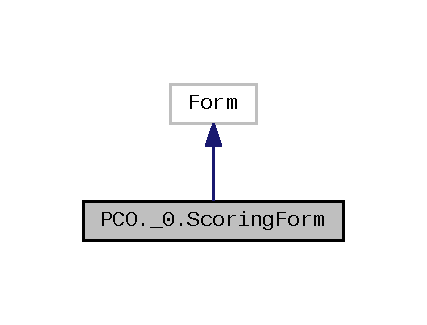
\includegraphics[width=205pt]{classPCO_1_1__0_1_1ScoringForm__inherit__graph}
\end{center}
\end{figure}


Collaboration diagram for P\+C\+O.\+\_\+0.\+Scoring\+Form\+:\nopagebreak
\begin{figure}[H]
\begin{center}
\leavevmode
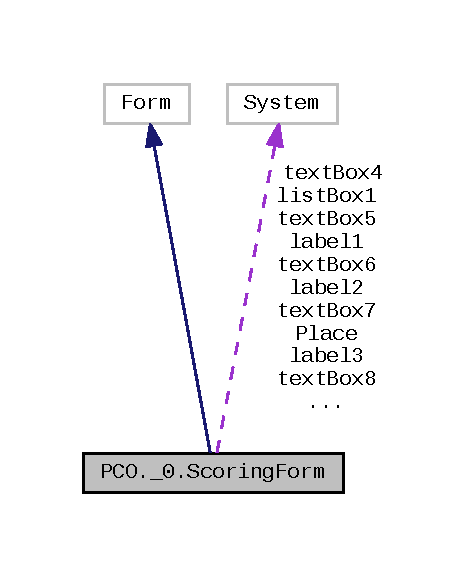
\includegraphics[width=225pt]{classPCO_1_1__0_1_1ScoringForm__coll__graph}
\end{center}
\end{figure}
\subsection*{Public Member Functions}
\begin{DoxyCompactItemize}
\item 
\hyperlink{classPCO_1_1__0_1_1ScoringForm_a853a6e4da6db5226f7536cee2faad9d0}{Scoring\+Form} ()
\end{DoxyCompactItemize}
\subsection*{Protected Member Functions}
\begin{DoxyCompactItemize}
\item 
override void \hyperlink{classPCO_1_1__0_1_1ScoringForm_aba931e2b82e00f2143ce9c1a19f84986}{Dispose} (bool disposing)
\begin{DoxyCompactList}\small\item\em Clean up any resources being used. \end{DoxyCompactList}\end{DoxyCompactItemize}
\subsection*{Private Member Functions}
\begin{DoxyCompactItemize}
\item 
void \hyperlink{classPCO_1_1__0_1_1ScoringForm_a58f4b35c1ec7a0f9480d832f50778891}{Form5\+\_\+\+Load} (object sender, Event\+Args e)
\item 
void \hyperlink{classPCO_1_1__0_1_1ScoringForm_a8600f55a40dd6b69fc8d455b027c96b7}{list\+Box1\+\_\+\+Selected\+Index\+Changed} (object sender, Event\+Args e)
\item 
void \hyperlink{classPCO_1_1__0_1_1ScoringForm_ac1be33466917df2d76628a4d302df722}{button1\+\_\+\+Click} (object sender, Event\+Args e)
\item 
void \hyperlink{classPCO_1_1__0_1_1ScoringForm_a7af8b812ae42aec0accb3c2760835a69}{data\+Grid\+View1\+\_\+\+Cell\+Content\+Click} (object sender, Data\+Grid\+View\+Cell\+Event\+Args e)
\item 
void \hyperlink{classPCO_1_1__0_1_1ScoringForm_a21264de2ba76e68e25c938d893ab8f6d}{button2\+\_\+\+Click} (object sender, Event\+Args e)
\item 
void \hyperlink{classPCO_1_1__0_1_1ScoringForm_aa05835d3b4c0eeecf783e6ef08c8a41e}{button3\+\_\+\+Click} (object sender, Event\+Args e)
\item 
void \hyperlink{classPCO_1_1__0_1_1ScoringForm_afc0d9d6e842d9fdf1eb59263d842ffee}{Initialize\+Component} ()
\begin{DoxyCompactList}\small\item\em Required method for Designer support -\/ do not modify the contents of this method with the code editor. \end{DoxyCompactList}\end{DoxyCompactItemize}
\subsection*{Private Attributes}
\begin{DoxyCompactItemize}
\item 
string \hyperlink{classPCO_1_1__0_1_1ScoringForm_aaa61029f62d413187283b96fa272b661}{Selected\+Event}
\item 
System.\+Component\+Model.\+I\+Container \hyperlink{classPCO_1_1__0_1_1ScoringForm_a238c9307e7ffe22b4d8e14a46a662ad7}{components} = null
\begin{DoxyCompactList}\small\item\em Required designer variable. \end{DoxyCompactList}\item 
System.\+Windows.\+Forms.\+Data\+Grid\+View \hyperlink{classPCO_1_1__0_1_1ScoringForm_a291143cc88a016f10f58fa7d048f9bfd}{data\+Grid\+View1}
\item 
System.\+Windows.\+Forms.\+List\+Box \hyperlink{classPCO_1_1__0_1_1ScoringForm_a1d8e561957cc9b2b1e8b8ba020146fa8}{list\+Box1}
\item 
System.\+Windows.\+Forms.\+Button \hyperlink{classPCO_1_1__0_1_1ScoringForm_ae18f67ae6a9b3ec07df6906ed58e6c86}{button1}
\item 
System.\+Windows.\+Forms.\+Label \hyperlink{classPCO_1_1__0_1_1ScoringForm_ae5175573b853fa4a41c932659ad4f849}{label1}
\item 
System.\+Windows.\+Forms.\+Label \hyperlink{classPCO_1_1__0_1_1ScoringForm_af0dd988c86ad1061fdec991c860c50ee}{label2}
\item 
System.\+Windows.\+Forms.\+Label \hyperlink{classPCO_1_1__0_1_1ScoringForm_adff715a0754a45263fda7bbf04d3d081}{label3}
\item 
System.\+Windows.\+Forms.\+Data\+Grid\+View\+Text\+Box\+Column \hyperlink{classPCO_1_1__0_1_1ScoringForm_a032fbd87d18a6e0907a83c282e4f2560}{Place}
\item 
System.\+Windows.\+Forms.\+Button \hyperlink{classPCO_1_1__0_1_1ScoringForm_a9313a2d479643918e22a9c40ce624e8f}{button2}
\item 
System.\+Windows.\+Forms.\+Text\+Box \hyperlink{classPCO_1_1__0_1_1ScoringForm_adc8b58eb57aed1d19dd9d44e5cfc910b}{text\+Box1}
\item 
System.\+Windows.\+Forms.\+Label \hyperlink{classPCO_1_1__0_1_1ScoringForm_afd53cf291beebbd1e52c6500f8d761bb}{label4}
\item 
System.\+Windows.\+Forms.\+Text\+Box \hyperlink{classPCO_1_1__0_1_1ScoringForm_a9b7dea60c839e9e490136e415cbca689}{text\+Box2}
\item 
System.\+Windows.\+Forms.\+Text\+Box \hyperlink{classPCO_1_1__0_1_1ScoringForm_a05ec3d37f45a4950e06b22c6974dcdbc}{text\+Box3}
\item 
System.\+Windows.\+Forms.\+Text\+Box \hyperlink{classPCO_1_1__0_1_1ScoringForm_a55e436955e52f177c61885d854da3a7d}{text\+Box4}
\item 
System.\+Windows.\+Forms.\+Text\+Box \hyperlink{classPCO_1_1__0_1_1ScoringForm_afccad5172710be1561f73c554d77ee59}{text\+Box5}
\item 
System.\+Windows.\+Forms.\+Text\+Box \hyperlink{classPCO_1_1__0_1_1ScoringForm_ae9fb74680f84b7e39a49625642aa1893}{text\+Box6}
\item 
System.\+Windows.\+Forms.\+Text\+Box \hyperlink{classPCO_1_1__0_1_1ScoringForm_a743b9df795f09a7afac4f252981cec70}{text\+Box7}
\item 
System.\+Windows.\+Forms.\+Text\+Box \hyperlink{classPCO_1_1__0_1_1ScoringForm_a1bdd53f49a48c5ce09d4f63365b7ecf4}{text\+Box8}
\item 
System.\+Windows.\+Forms.\+Button \hyperlink{classPCO_1_1__0_1_1ScoringForm_aaa0f5bd68251cbe3438f04f85c04b592}{button3}
\item 
System.\+Windows.\+Forms.\+Label \hyperlink{classPCO_1_1__0_1_1ScoringForm_ace66a75e3f343acdb65cc68d14b8ac2e}{label5}
\item 
System.\+Windows.\+Forms.\+Label \hyperlink{classPCO_1_1__0_1_1ScoringForm_aaa5fb477595b697132491cdac72ec1a5}{label6}
\item 
System.\+Windows.\+Forms.\+Label \hyperlink{classPCO_1_1__0_1_1ScoringForm_acf22d3bbb1a14fefc2fe9b90ee685619}{label7}
\end{DoxyCompactItemize}


\subsection{Detailed Description}
\hyperlink{classScoring}{Scoring} class for G\+UI. 

Definition at line 15 of file Judge.\+cs.



\subsection{Constructor \& Destructor Documentation}
\mbox{\Hypertarget{classPCO_1_1__0_1_1ScoringForm_a853a6e4da6db5226f7536cee2faad9d0}\label{classPCO_1_1__0_1_1ScoringForm_a853a6e4da6db5226f7536cee2faad9d0}} 
\index{P\+C\+O\+::\+\_\+0\+::\+Scoring\+Form@{P\+C\+O\+::\+\_\+0\+::\+Scoring\+Form}!Scoring\+Form@{Scoring\+Form}}
\index{Scoring\+Form@{Scoring\+Form}!P\+C\+O\+::\+\_\+0\+::\+Scoring\+Form@{P\+C\+O\+::\+\_\+0\+::\+Scoring\+Form}}
\subsubsection{\texorpdfstring{Scoring\+Form()}{ScoringForm()}}
{\footnotesize\ttfamily P\+C\+O.\+\_\+0.\+Scoring\+Form.\+Scoring\+Form (\begin{DoxyParamCaption}{ }\end{DoxyParamCaption})\hspace{0.3cm}{\ttfamily [inline]}}



Definition at line 18 of file Judge.\+cs.



\subsection{Member Function Documentation}
\mbox{\Hypertarget{classPCO_1_1__0_1_1ScoringForm_ac1be33466917df2d76628a4d302df722}\label{classPCO_1_1__0_1_1ScoringForm_ac1be33466917df2d76628a4d302df722}} 
\index{P\+C\+O\+::\+\_\+0\+::\+Scoring\+Form@{P\+C\+O\+::\+\_\+0\+::\+Scoring\+Form}!button1\+\_\+\+Click@{button1\+\_\+\+Click}}
\index{button1\+\_\+\+Click@{button1\+\_\+\+Click}!P\+C\+O\+::\+\_\+0\+::\+Scoring\+Form@{P\+C\+O\+::\+\_\+0\+::\+Scoring\+Form}}
\subsubsection{\texorpdfstring{button1\+\_\+\+Click()}{button1\_Click()}}
{\footnotesize\ttfamily void P\+C\+O.\+\_\+0.\+Scoring\+Form.\+button1\+\_\+\+Click (\begin{DoxyParamCaption}\item[{object}]{sender,  }\item[{Event\+Args}]{e }\end{DoxyParamCaption})\hspace{0.3cm}{\ttfamily [inline]}, {\ttfamily [private]}}



Definition at line 72 of file Judge.\+cs.

\mbox{\Hypertarget{classPCO_1_1__0_1_1ScoringForm_a21264de2ba76e68e25c938d893ab8f6d}\label{classPCO_1_1__0_1_1ScoringForm_a21264de2ba76e68e25c938d893ab8f6d}} 
\index{P\+C\+O\+::\+\_\+0\+::\+Scoring\+Form@{P\+C\+O\+::\+\_\+0\+::\+Scoring\+Form}!button2\+\_\+\+Click@{button2\+\_\+\+Click}}
\index{button2\+\_\+\+Click@{button2\+\_\+\+Click}!P\+C\+O\+::\+\_\+0\+::\+Scoring\+Form@{P\+C\+O\+::\+\_\+0\+::\+Scoring\+Form}}
\subsubsection{\texorpdfstring{button2\+\_\+\+Click()}{button2\_Click()}}
{\footnotesize\ttfamily void P\+C\+O.\+\_\+0.\+Scoring\+Form.\+button2\+\_\+\+Click (\begin{DoxyParamCaption}\item[{object}]{sender,  }\item[{Event\+Args}]{e }\end{DoxyParamCaption})\hspace{0.3cm}{\ttfamily [inline]}, {\ttfamily [private]}}



Definition at line 612 of file Judge.\+cs.

\mbox{\Hypertarget{classPCO_1_1__0_1_1ScoringForm_aa05835d3b4c0eeecf783e6ef08c8a41e}\label{classPCO_1_1__0_1_1ScoringForm_aa05835d3b4c0eeecf783e6ef08c8a41e}} 
\index{P\+C\+O\+::\+\_\+0\+::\+Scoring\+Form@{P\+C\+O\+::\+\_\+0\+::\+Scoring\+Form}!button3\+\_\+\+Click@{button3\+\_\+\+Click}}
\index{button3\+\_\+\+Click@{button3\+\_\+\+Click}!P\+C\+O\+::\+\_\+0\+::\+Scoring\+Form@{P\+C\+O\+::\+\_\+0\+::\+Scoring\+Form}}
\subsubsection{\texorpdfstring{button3\+\_\+\+Click()}{button3\_Click()}}
{\footnotesize\ttfamily void P\+C\+O.\+\_\+0.\+Scoring\+Form.\+button3\+\_\+\+Click (\begin{DoxyParamCaption}\item[{object}]{sender,  }\item[{Event\+Args}]{e }\end{DoxyParamCaption})\hspace{0.3cm}{\ttfamily [inline]}, {\ttfamily [private]}}



Definition at line 649 of file Judge.\+cs.

\mbox{\Hypertarget{classPCO_1_1__0_1_1ScoringForm_a7af8b812ae42aec0accb3c2760835a69}\label{classPCO_1_1__0_1_1ScoringForm_a7af8b812ae42aec0accb3c2760835a69}} 
\index{P\+C\+O\+::\+\_\+0\+::\+Scoring\+Form@{P\+C\+O\+::\+\_\+0\+::\+Scoring\+Form}!data\+Grid\+View1\+\_\+\+Cell\+Content\+Click@{data\+Grid\+View1\+\_\+\+Cell\+Content\+Click}}
\index{data\+Grid\+View1\+\_\+\+Cell\+Content\+Click@{data\+Grid\+View1\+\_\+\+Cell\+Content\+Click}!P\+C\+O\+::\+\_\+0\+::\+Scoring\+Form@{P\+C\+O\+::\+\_\+0\+::\+Scoring\+Form}}
\subsubsection{\texorpdfstring{data\+Grid\+View1\+\_\+\+Cell\+Content\+Click()}{dataGridView1\_CellContentClick()}}
{\footnotesize\ttfamily void P\+C\+O.\+\_\+0.\+Scoring\+Form.\+data\+Grid\+View1\+\_\+\+Cell\+Content\+Click (\begin{DoxyParamCaption}\item[{object}]{sender,  }\item[{Data\+Grid\+View\+Cell\+Event\+Args}]{e }\end{DoxyParamCaption})\hspace{0.3cm}{\ttfamily [inline]}, {\ttfamily [private]}}



Definition at line 607 of file Judge.\+cs.

\mbox{\Hypertarget{classPCO_1_1__0_1_1ScoringForm_aba931e2b82e00f2143ce9c1a19f84986}\label{classPCO_1_1__0_1_1ScoringForm_aba931e2b82e00f2143ce9c1a19f84986}} 
\index{P\+C\+O\+::\+\_\+0\+::\+Scoring\+Form@{P\+C\+O\+::\+\_\+0\+::\+Scoring\+Form}!Dispose@{Dispose}}
\index{Dispose@{Dispose}!P\+C\+O\+::\+\_\+0\+::\+Scoring\+Form@{P\+C\+O\+::\+\_\+0\+::\+Scoring\+Form}}
\subsubsection{\texorpdfstring{Dispose()}{Dispose()}}
{\footnotesize\ttfamily override void P\+C\+O.\+\_\+0.\+Scoring\+Form.\+Dispose (\begin{DoxyParamCaption}\item[{bool}]{disposing }\end{DoxyParamCaption})\hspace{0.3cm}{\ttfamily [inline]}, {\ttfamily [protected]}}



Clean up any resources being used. 


\begin{DoxyParams}{Parameters}
{\em disposing} & true if managed resources should be disposed; otherwise, false.\\
\hline
\end{DoxyParams}


Definition at line 14 of file Judge.\+Designer.\+cs.

\mbox{\Hypertarget{classPCO_1_1__0_1_1ScoringForm_a58f4b35c1ec7a0f9480d832f50778891}\label{classPCO_1_1__0_1_1ScoringForm_a58f4b35c1ec7a0f9480d832f50778891}} 
\index{P\+C\+O\+::\+\_\+0\+::\+Scoring\+Form@{P\+C\+O\+::\+\_\+0\+::\+Scoring\+Form}!Form5\+\_\+\+Load@{Form5\+\_\+\+Load}}
\index{Form5\+\_\+\+Load@{Form5\+\_\+\+Load}!P\+C\+O\+::\+\_\+0\+::\+Scoring\+Form@{P\+C\+O\+::\+\_\+0\+::\+Scoring\+Form}}
\subsubsection{\texorpdfstring{Form5\+\_\+\+Load()}{Form5\_Load()}}
{\footnotesize\ttfamily void P\+C\+O.\+\_\+0.\+Scoring\+Form.\+Form5\+\_\+\+Load (\begin{DoxyParamCaption}\item[{object}]{sender,  }\item[{Event\+Args}]{e }\end{DoxyParamCaption})\hspace{0.3cm}{\ttfamily [inline]}, {\ttfamily [private]}}



Definition at line 23 of file Judge.\+cs.

\mbox{\Hypertarget{classPCO_1_1__0_1_1ScoringForm_afc0d9d6e842d9fdf1eb59263d842ffee}\label{classPCO_1_1__0_1_1ScoringForm_afc0d9d6e842d9fdf1eb59263d842ffee}} 
\index{P\+C\+O\+::\+\_\+0\+::\+Scoring\+Form@{P\+C\+O\+::\+\_\+0\+::\+Scoring\+Form}!Initialize\+Component@{Initialize\+Component}}
\index{Initialize\+Component@{Initialize\+Component}!P\+C\+O\+::\+\_\+0\+::\+Scoring\+Form@{P\+C\+O\+::\+\_\+0\+::\+Scoring\+Form}}
\subsubsection{\texorpdfstring{Initialize\+Component()}{InitializeComponent()}}
{\footnotesize\ttfamily void P\+C\+O.\+\_\+0.\+Scoring\+Form.\+Initialize\+Component (\begin{DoxyParamCaption}{ }\end{DoxyParamCaption})\hspace{0.3cm}{\ttfamily [inline]}, {\ttfamily [private]}}



Required method for Designer support -\/ do not modify the contents of this method with the code editor. 



Definition at line 29 of file Judge.\+Designer.\+cs.

\mbox{\Hypertarget{classPCO_1_1__0_1_1ScoringForm_a8600f55a40dd6b69fc8d455b027c96b7}\label{classPCO_1_1__0_1_1ScoringForm_a8600f55a40dd6b69fc8d455b027c96b7}} 
\index{P\+C\+O\+::\+\_\+0\+::\+Scoring\+Form@{P\+C\+O\+::\+\_\+0\+::\+Scoring\+Form}!list\+Box1\+\_\+\+Selected\+Index\+Changed@{list\+Box1\+\_\+\+Selected\+Index\+Changed}}
\index{list\+Box1\+\_\+\+Selected\+Index\+Changed@{list\+Box1\+\_\+\+Selected\+Index\+Changed}!P\+C\+O\+::\+\_\+0\+::\+Scoring\+Form@{P\+C\+O\+::\+\_\+0\+::\+Scoring\+Form}}
\subsubsection{\texorpdfstring{list\+Box1\+\_\+\+Selected\+Index\+Changed()}{listBox1\_SelectedIndexChanged()}}
{\footnotesize\ttfamily void P\+C\+O.\+\_\+0.\+Scoring\+Form.\+list\+Box1\+\_\+\+Selected\+Index\+Changed (\begin{DoxyParamCaption}\item[{object}]{sender,  }\item[{Event\+Args}]{e }\end{DoxyParamCaption})\hspace{0.3cm}{\ttfamily [inline]}, {\ttfamily [private]}}



Definition at line 67 of file Judge.\+cs.



\subsection{Member Data Documentation}
\mbox{\Hypertarget{classPCO_1_1__0_1_1ScoringForm_ae18f67ae6a9b3ec07df6906ed58e6c86}\label{classPCO_1_1__0_1_1ScoringForm_ae18f67ae6a9b3ec07df6906ed58e6c86}} 
\index{P\+C\+O\+::\+\_\+0\+::\+Scoring\+Form@{P\+C\+O\+::\+\_\+0\+::\+Scoring\+Form}!button1@{button1}}
\index{button1@{button1}!P\+C\+O\+::\+\_\+0\+::\+Scoring\+Form@{P\+C\+O\+::\+\_\+0\+::\+Scoring\+Form}}
\subsubsection{\texorpdfstring{button1}{button1}}
{\footnotesize\ttfamily System.\+Windows.\+Forms.\+Button P\+C\+O.\+\_\+0.\+Scoring\+Form.\+button1\hspace{0.3cm}{\ttfamily [private]}}



Definition at line 286 of file Judge.\+Designer.\+cs.

\mbox{\Hypertarget{classPCO_1_1__0_1_1ScoringForm_a9313a2d479643918e22a9c40ce624e8f}\label{classPCO_1_1__0_1_1ScoringForm_a9313a2d479643918e22a9c40ce624e8f}} 
\index{P\+C\+O\+::\+\_\+0\+::\+Scoring\+Form@{P\+C\+O\+::\+\_\+0\+::\+Scoring\+Form}!button2@{button2}}
\index{button2@{button2}!P\+C\+O\+::\+\_\+0\+::\+Scoring\+Form@{P\+C\+O\+::\+\_\+0\+::\+Scoring\+Form}}
\subsubsection{\texorpdfstring{button2}{button2}}
{\footnotesize\ttfamily System.\+Windows.\+Forms.\+Button P\+C\+O.\+\_\+0.\+Scoring\+Form.\+button2\hspace{0.3cm}{\ttfamily [private]}}



Definition at line 291 of file Judge.\+Designer.\+cs.

\mbox{\Hypertarget{classPCO_1_1__0_1_1ScoringForm_aaa0f5bd68251cbe3438f04f85c04b592}\label{classPCO_1_1__0_1_1ScoringForm_aaa0f5bd68251cbe3438f04f85c04b592}} 
\index{P\+C\+O\+::\+\_\+0\+::\+Scoring\+Form@{P\+C\+O\+::\+\_\+0\+::\+Scoring\+Form}!button3@{button3}}
\index{button3@{button3}!P\+C\+O\+::\+\_\+0\+::\+Scoring\+Form@{P\+C\+O\+::\+\_\+0\+::\+Scoring\+Form}}
\subsubsection{\texorpdfstring{button3}{button3}}
{\footnotesize\ttfamily System.\+Windows.\+Forms.\+Button P\+C\+O.\+\_\+0.\+Scoring\+Form.\+button3\hspace{0.3cm}{\ttfamily [private]}}



Definition at line 301 of file Judge.\+Designer.\+cs.

\mbox{\Hypertarget{classPCO_1_1__0_1_1ScoringForm_a238c9307e7ffe22b4d8e14a46a662ad7}\label{classPCO_1_1__0_1_1ScoringForm_a238c9307e7ffe22b4d8e14a46a662ad7}} 
\index{P\+C\+O\+::\+\_\+0\+::\+Scoring\+Form@{P\+C\+O\+::\+\_\+0\+::\+Scoring\+Form}!components@{components}}
\index{components@{components}!P\+C\+O\+::\+\_\+0\+::\+Scoring\+Form@{P\+C\+O\+::\+\_\+0\+::\+Scoring\+Form}}
\subsubsection{\texorpdfstring{components}{components}}
{\footnotesize\ttfamily System.\+Component\+Model.\+I\+Container P\+C\+O.\+\_\+0.\+Scoring\+Form.\+components = null\hspace{0.3cm}{\ttfamily [private]}}



Required designer variable. 



Definition at line 8 of file Judge.\+Designer.\+cs.

\mbox{\Hypertarget{classPCO_1_1__0_1_1ScoringForm_a291143cc88a016f10f58fa7d048f9bfd}\label{classPCO_1_1__0_1_1ScoringForm_a291143cc88a016f10f58fa7d048f9bfd}} 
\index{P\+C\+O\+::\+\_\+0\+::\+Scoring\+Form@{P\+C\+O\+::\+\_\+0\+::\+Scoring\+Form}!data\+Grid\+View1@{data\+Grid\+View1}}
\index{data\+Grid\+View1@{data\+Grid\+View1}!P\+C\+O\+::\+\_\+0\+::\+Scoring\+Form@{P\+C\+O\+::\+\_\+0\+::\+Scoring\+Form}}
\subsubsection{\texorpdfstring{data\+Grid\+View1}{dataGridView1}}
{\footnotesize\ttfamily System.\+Windows.\+Forms.\+Data\+Grid\+View P\+C\+O.\+\_\+0.\+Scoring\+Form.\+data\+Grid\+View1\hspace{0.3cm}{\ttfamily [private]}}



Definition at line 284 of file Judge.\+Designer.\+cs.

\mbox{\Hypertarget{classPCO_1_1__0_1_1ScoringForm_ae5175573b853fa4a41c932659ad4f849}\label{classPCO_1_1__0_1_1ScoringForm_ae5175573b853fa4a41c932659ad4f849}} 
\index{P\+C\+O\+::\+\_\+0\+::\+Scoring\+Form@{P\+C\+O\+::\+\_\+0\+::\+Scoring\+Form}!label1@{label1}}
\index{label1@{label1}!P\+C\+O\+::\+\_\+0\+::\+Scoring\+Form@{P\+C\+O\+::\+\_\+0\+::\+Scoring\+Form}}
\subsubsection{\texorpdfstring{label1}{label1}}
{\footnotesize\ttfamily System.\+Windows.\+Forms.\+Label P\+C\+O.\+\_\+0.\+Scoring\+Form.\+label1\hspace{0.3cm}{\ttfamily [private]}}



Definition at line 287 of file Judge.\+Designer.\+cs.

\mbox{\Hypertarget{classPCO_1_1__0_1_1ScoringForm_af0dd988c86ad1061fdec991c860c50ee}\label{classPCO_1_1__0_1_1ScoringForm_af0dd988c86ad1061fdec991c860c50ee}} 
\index{P\+C\+O\+::\+\_\+0\+::\+Scoring\+Form@{P\+C\+O\+::\+\_\+0\+::\+Scoring\+Form}!label2@{label2}}
\index{label2@{label2}!P\+C\+O\+::\+\_\+0\+::\+Scoring\+Form@{P\+C\+O\+::\+\_\+0\+::\+Scoring\+Form}}
\subsubsection{\texorpdfstring{label2}{label2}}
{\footnotesize\ttfamily System.\+Windows.\+Forms.\+Label P\+C\+O.\+\_\+0.\+Scoring\+Form.\+label2\hspace{0.3cm}{\ttfamily [private]}}



Definition at line 288 of file Judge.\+Designer.\+cs.

\mbox{\Hypertarget{classPCO_1_1__0_1_1ScoringForm_adff715a0754a45263fda7bbf04d3d081}\label{classPCO_1_1__0_1_1ScoringForm_adff715a0754a45263fda7bbf04d3d081}} 
\index{P\+C\+O\+::\+\_\+0\+::\+Scoring\+Form@{P\+C\+O\+::\+\_\+0\+::\+Scoring\+Form}!label3@{label3}}
\index{label3@{label3}!P\+C\+O\+::\+\_\+0\+::\+Scoring\+Form@{P\+C\+O\+::\+\_\+0\+::\+Scoring\+Form}}
\subsubsection{\texorpdfstring{label3}{label3}}
{\footnotesize\ttfamily System.\+Windows.\+Forms.\+Label P\+C\+O.\+\_\+0.\+Scoring\+Form.\+label3\hspace{0.3cm}{\ttfamily [private]}}



Definition at line 289 of file Judge.\+Designer.\+cs.

\mbox{\Hypertarget{classPCO_1_1__0_1_1ScoringForm_afd53cf291beebbd1e52c6500f8d761bb}\label{classPCO_1_1__0_1_1ScoringForm_afd53cf291beebbd1e52c6500f8d761bb}} 
\index{P\+C\+O\+::\+\_\+0\+::\+Scoring\+Form@{P\+C\+O\+::\+\_\+0\+::\+Scoring\+Form}!label4@{label4}}
\index{label4@{label4}!P\+C\+O\+::\+\_\+0\+::\+Scoring\+Form@{P\+C\+O\+::\+\_\+0\+::\+Scoring\+Form}}
\subsubsection{\texorpdfstring{label4}{label4}}
{\footnotesize\ttfamily System.\+Windows.\+Forms.\+Label P\+C\+O.\+\_\+0.\+Scoring\+Form.\+label4\hspace{0.3cm}{\ttfamily [private]}}



Definition at line 293 of file Judge.\+Designer.\+cs.

\mbox{\Hypertarget{classPCO_1_1__0_1_1ScoringForm_ace66a75e3f343acdb65cc68d14b8ac2e}\label{classPCO_1_1__0_1_1ScoringForm_ace66a75e3f343acdb65cc68d14b8ac2e}} 
\index{P\+C\+O\+::\+\_\+0\+::\+Scoring\+Form@{P\+C\+O\+::\+\_\+0\+::\+Scoring\+Form}!label5@{label5}}
\index{label5@{label5}!P\+C\+O\+::\+\_\+0\+::\+Scoring\+Form@{P\+C\+O\+::\+\_\+0\+::\+Scoring\+Form}}
\subsubsection{\texorpdfstring{label5}{label5}}
{\footnotesize\ttfamily System.\+Windows.\+Forms.\+Label P\+C\+O.\+\_\+0.\+Scoring\+Form.\+label5\hspace{0.3cm}{\ttfamily [private]}}



Definition at line 302 of file Judge.\+Designer.\+cs.

\mbox{\Hypertarget{classPCO_1_1__0_1_1ScoringForm_aaa5fb477595b697132491cdac72ec1a5}\label{classPCO_1_1__0_1_1ScoringForm_aaa5fb477595b697132491cdac72ec1a5}} 
\index{P\+C\+O\+::\+\_\+0\+::\+Scoring\+Form@{P\+C\+O\+::\+\_\+0\+::\+Scoring\+Form}!label6@{label6}}
\index{label6@{label6}!P\+C\+O\+::\+\_\+0\+::\+Scoring\+Form@{P\+C\+O\+::\+\_\+0\+::\+Scoring\+Form}}
\subsubsection{\texorpdfstring{label6}{label6}}
{\footnotesize\ttfamily System.\+Windows.\+Forms.\+Label P\+C\+O.\+\_\+0.\+Scoring\+Form.\+label6\hspace{0.3cm}{\ttfamily [private]}}



Definition at line 303 of file Judge.\+Designer.\+cs.

\mbox{\Hypertarget{classPCO_1_1__0_1_1ScoringForm_acf22d3bbb1a14fefc2fe9b90ee685619}\label{classPCO_1_1__0_1_1ScoringForm_acf22d3bbb1a14fefc2fe9b90ee685619}} 
\index{P\+C\+O\+::\+\_\+0\+::\+Scoring\+Form@{P\+C\+O\+::\+\_\+0\+::\+Scoring\+Form}!label7@{label7}}
\index{label7@{label7}!P\+C\+O\+::\+\_\+0\+::\+Scoring\+Form@{P\+C\+O\+::\+\_\+0\+::\+Scoring\+Form}}
\subsubsection{\texorpdfstring{label7}{label7}}
{\footnotesize\ttfamily System.\+Windows.\+Forms.\+Label P\+C\+O.\+\_\+0.\+Scoring\+Form.\+label7\hspace{0.3cm}{\ttfamily [private]}}



Definition at line 304 of file Judge.\+Designer.\+cs.

\mbox{\Hypertarget{classPCO_1_1__0_1_1ScoringForm_a1d8e561957cc9b2b1e8b8ba020146fa8}\label{classPCO_1_1__0_1_1ScoringForm_a1d8e561957cc9b2b1e8b8ba020146fa8}} 
\index{P\+C\+O\+::\+\_\+0\+::\+Scoring\+Form@{P\+C\+O\+::\+\_\+0\+::\+Scoring\+Form}!list\+Box1@{list\+Box1}}
\index{list\+Box1@{list\+Box1}!P\+C\+O\+::\+\_\+0\+::\+Scoring\+Form@{P\+C\+O\+::\+\_\+0\+::\+Scoring\+Form}}
\subsubsection{\texorpdfstring{list\+Box1}{listBox1}}
{\footnotesize\ttfamily System.\+Windows.\+Forms.\+List\+Box P\+C\+O.\+\_\+0.\+Scoring\+Form.\+list\+Box1\hspace{0.3cm}{\ttfamily [private]}}



Definition at line 285 of file Judge.\+Designer.\+cs.

\mbox{\Hypertarget{classPCO_1_1__0_1_1ScoringForm_a032fbd87d18a6e0907a83c282e4f2560}\label{classPCO_1_1__0_1_1ScoringForm_a032fbd87d18a6e0907a83c282e4f2560}} 
\index{P\+C\+O\+::\+\_\+0\+::\+Scoring\+Form@{P\+C\+O\+::\+\_\+0\+::\+Scoring\+Form}!Place@{Place}}
\index{Place@{Place}!P\+C\+O\+::\+\_\+0\+::\+Scoring\+Form@{P\+C\+O\+::\+\_\+0\+::\+Scoring\+Form}}
\subsubsection{\texorpdfstring{Place}{Place}}
{\footnotesize\ttfamily System.\+Windows.\+Forms.\+Data\+Grid\+View\+Text\+Box\+Column P\+C\+O.\+\_\+0.\+Scoring\+Form.\+Place\hspace{0.3cm}{\ttfamily [private]}}



Definition at line 290 of file Judge.\+Designer.\+cs.

\mbox{\Hypertarget{classPCO_1_1__0_1_1ScoringForm_aaa61029f62d413187283b96fa272b661}\label{classPCO_1_1__0_1_1ScoringForm_aaa61029f62d413187283b96fa272b661}} 
\index{P\+C\+O\+::\+\_\+0\+::\+Scoring\+Form@{P\+C\+O\+::\+\_\+0\+::\+Scoring\+Form}!Selected\+Event@{Selected\+Event}}
\index{Selected\+Event@{Selected\+Event}!P\+C\+O\+::\+\_\+0\+::\+Scoring\+Form@{P\+C\+O\+::\+\_\+0\+::\+Scoring\+Form}}
\subsubsection{\texorpdfstring{Selected\+Event}{SelectedEvent}}
{\footnotesize\ttfamily string P\+C\+O.\+\_\+0.\+Scoring\+Form.\+Selected\+Event\hspace{0.3cm}{\ttfamily [private]}}



Definition at line 17 of file Judge.\+cs.

\mbox{\Hypertarget{classPCO_1_1__0_1_1ScoringForm_adc8b58eb57aed1d19dd9d44e5cfc910b}\label{classPCO_1_1__0_1_1ScoringForm_adc8b58eb57aed1d19dd9d44e5cfc910b}} 
\index{P\+C\+O\+::\+\_\+0\+::\+Scoring\+Form@{P\+C\+O\+::\+\_\+0\+::\+Scoring\+Form}!text\+Box1@{text\+Box1}}
\index{text\+Box1@{text\+Box1}!P\+C\+O\+::\+\_\+0\+::\+Scoring\+Form@{P\+C\+O\+::\+\_\+0\+::\+Scoring\+Form}}
\subsubsection{\texorpdfstring{text\+Box1}{textBox1}}
{\footnotesize\ttfamily System.\+Windows.\+Forms.\+Text\+Box P\+C\+O.\+\_\+0.\+Scoring\+Form.\+text\+Box1\hspace{0.3cm}{\ttfamily [private]}}



Definition at line 292 of file Judge.\+Designer.\+cs.

\mbox{\Hypertarget{classPCO_1_1__0_1_1ScoringForm_a9b7dea60c839e9e490136e415cbca689}\label{classPCO_1_1__0_1_1ScoringForm_a9b7dea60c839e9e490136e415cbca689}} 
\index{P\+C\+O\+::\+\_\+0\+::\+Scoring\+Form@{P\+C\+O\+::\+\_\+0\+::\+Scoring\+Form}!text\+Box2@{text\+Box2}}
\index{text\+Box2@{text\+Box2}!P\+C\+O\+::\+\_\+0\+::\+Scoring\+Form@{P\+C\+O\+::\+\_\+0\+::\+Scoring\+Form}}
\subsubsection{\texorpdfstring{text\+Box2}{textBox2}}
{\footnotesize\ttfamily System.\+Windows.\+Forms.\+Text\+Box P\+C\+O.\+\_\+0.\+Scoring\+Form.\+text\+Box2\hspace{0.3cm}{\ttfamily [private]}}



Definition at line 294 of file Judge.\+Designer.\+cs.

\mbox{\Hypertarget{classPCO_1_1__0_1_1ScoringForm_a05ec3d37f45a4950e06b22c6974dcdbc}\label{classPCO_1_1__0_1_1ScoringForm_a05ec3d37f45a4950e06b22c6974dcdbc}} 
\index{P\+C\+O\+::\+\_\+0\+::\+Scoring\+Form@{P\+C\+O\+::\+\_\+0\+::\+Scoring\+Form}!text\+Box3@{text\+Box3}}
\index{text\+Box3@{text\+Box3}!P\+C\+O\+::\+\_\+0\+::\+Scoring\+Form@{P\+C\+O\+::\+\_\+0\+::\+Scoring\+Form}}
\subsubsection{\texorpdfstring{text\+Box3}{textBox3}}
{\footnotesize\ttfamily System.\+Windows.\+Forms.\+Text\+Box P\+C\+O.\+\_\+0.\+Scoring\+Form.\+text\+Box3\hspace{0.3cm}{\ttfamily [private]}}



Definition at line 295 of file Judge.\+Designer.\+cs.

\mbox{\Hypertarget{classPCO_1_1__0_1_1ScoringForm_a55e436955e52f177c61885d854da3a7d}\label{classPCO_1_1__0_1_1ScoringForm_a55e436955e52f177c61885d854da3a7d}} 
\index{P\+C\+O\+::\+\_\+0\+::\+Scoring\+Form@{P\+C\+O\+::\+\_\+0\+::\+Scoring\+Form}!text\+Box4@{text\+Box4}}
\index{text\+Box4@{text\+Box4}!P\+C\+O\+::\+\_\+0\+::\+Scoring\+Form@{P\+C\+O\+::\+\_\+0\+::\+Scoring\+Form}}
\subsubsection{\texorpdfstring{text\+Box4}{textBox4}}
{\footnotesize\ttfamily System.\+Windows.\+Forms.\+Text\+Box P\+C\+O.\+\_\+0.\+Scoring\+Form.\+text\+Box4\hspace{0.3cm}{\ttfamily [private]}}



Definition at line 296 of file Judge.\+Designer.\+cs.

\mbox{\Hypertarget{classPCO_1_1__0_1_1ScoringForm_afccad5172710be1561f73c554d77ee59}\label{classPCO_1_1__0_1_1ScoringForm_afccad5172710be1561f73c554d77ee59}} 
\index{P\+C\+O\+::\+\_\+0\+::\+Scoring\+Form@{P\+C\+O\+::\+\_\+0\+::\+Scoring\+Form}!text\+Box5@{text\+Box5}}
\index{text\+Box5@{text\+Box5}!P\+C\+O\+::\+\_\+0\+::\+Scoring\+Form@{P\+C\+O\+::\+\_\+0\+::\+Scoring\+Form}}
\subsubsection{\texorpdfstring{text\+Box5}{textBox5}}
{\footnotesize\ttfamily System.\+Windows.\+Forms.\+Text\+Box P\+C\+O.\+\_\+0.\+Scoring\+Form.\+text\+Box5\hspace{0.3cm}{\ttfamily [private]}}



Definition at line 297 of file Judge.\+Designer.\+cs.

\mbox{\Hypertarget{classPCO_1_1__0_1_1ScoringForm_ae9fb74680f84b7e39a49625642aa1893}\label{classPCO_1_1__0_1_1ScoringForm_ae9fb74680f84b7e39a49625642aa1893}} 
\index{P\+C\+O\+::\+\_\+0\+::\+Scoring\+Form@{P\+C\+O\+::\+\_\+0\+::\+Scoring\+Form}!text\+Box6@{text\+Box6}}
\index{text\+Box6@{text\+Box6}!P\+C\+O\+::\+\_\+0\+::\+Scoring\+Form@{P\+C\+O\+::\+\_\+0\+::\+Scoring\+Form}}
\subsubsection{\texorpdfstring{text\+Box6}{textBox6}}
{\footnotesize\ttfamily System.\+Windows.\+Forms.\+Text\+Box P\+C\+O.\+\_\+0.\+Scoring\+Form.\+text\+Box6\hspace{0.3cm}{\ttfamily [private]}}



Definition at line 298 of file Judge.\+Designer.\+cs.

\mbox{\Hypertarget{classPCO_1_1__0_1_1ScoringForm_a743b9df795f09a7afac4f252981cec70}\label{classPCO_1_1__0_1_1ScoringForm_a743b9df795f09a7afac4f252981cec70}} 
\index{P\+C\+O\+::\+\_\+0\+::\+Scoring\+Form@{P\+C\+O\+::\+\_\+0\+::\+Scoring\+Form}!text\+Box7@{text\+Box7}}
\index{text\+Box7@{text\+Box7}!P\+C\+O\+::\+\_\+0\+::\+Scoring\+Form@{P\+C\+O\+::\+\_\+0\+::\+Scoring\+Form}}
\subsubsection{\texorpdfstring{text\+Box7}{textBox7}}
{\footnotesize\ttfamily System.\+Windows.\+Forms.\+Text\+Box P\+C\+O.\+\_\+0.\+Scoring\+Form.\+text\+Box7\hspace{0.3cm}{\ttfamily [private]}}



Definition at line 299 of file Judge.\+Designer.\+cs.

\mbox{\Hypertarget{classPCO_1_1__0_1_1ScoringForm_a1bdd53f49a48c5ce09d4f63365b7ecf4}\label{classPCO_1_1__0_1_1ScoringForm_a1bdd53f49a48c5ce09d4f63365b7ecf4}} 
\index{P\+C\+O\+::\+\_\+0\+::\+Scoring\+Form@{P\+C\+O\+::\+\_\+0\+::\+Scoring\+Form}!text\+Box8@{text\+Box8}}
\index{text\+Box8@{text\+Box8}!P\+C\+O\+::\+\_\+0\+::\+Scoring\+Form@{P\+C\+O\+::\+\_\+0\+::\+Scoring\+Form}}
\subsubsection{\texorpdfstring{text\+Box8}{textBox8}}
{\footnotesize\ttfamily System.\+Windows.\+Forms.\+Text\+Box P\+C\+O.\+\_\+0.\+Scoring\+Form.\+text\+Box8\hspace{0.3cm}{\ttfamily [private]}}



Definition at line 300 of file Judge.\+Designer.\+cs.



The documentation for this class was generated from the following files\+:\begin{DoxyCompactItemize}
\item 
\hyperlink{Judge_8cs}{Judge.\+cs}\item 
\hyperlink{Judge_8Designer_8cs}{Judge.\+Designer.\+cs}\end{DoxyCompactItemize}

\hypertarget{classSingleSkating}{}\section{Single\+Skating Class Reference}
\label{classSingleSkating}\index{Single\+Skating@{Single\+Skating}}


\hyperlink{classSingleSkating}{Single\+Skating} class is one of the 3 Figure\+Skating events.  


\subsection*{Public Member Functions}
\begin{DoxyCompactItemize}
\item 
\hyperlink{classSingleSkating_af9d28072daf32072d6169079cfeb6d68}{Single\+Skating} ()
\item 
void \hyperlink{classSingleSkating_a5af177900da74048cda071514a38339b}{Add\+Athlete\+Male} (string country, string Fname, string Lname)
\item 
void \hyperlink{classSingleSkating_a8b0ede01071b657b05037ccccc114ffe}{Add\+Athlete\+Female} (string country, string Fname, string Lname)
\end{DoxyCompactItemize}


\subsection{Detailed Description}
\hyperlink{classSingleSkating}{Single\+Skating} class is one of the 3 Figure\+Skating events. 

D\+E\+F\+I\+N\+I\+T\+I\+ON\+: Form of figure skating where athletes participate individually. The utilization of long program style where each athlete is free to do their own unique performance complete with technical tricks is present.

C\+O\+N\+S\+T\+R\+A\+I\+N\+TS\+: Each athlete performs solo on the rink at a given time. Total duration of performance is 4 minutes and 30 seconds.\begin{DoxyAuthor}{Author}
Landen Marchand 
\end{DoxyAuthor}


Definition at line 780 of file Class1.\+cs.



\subsection{Constructor \& Destructor Documentation}
\mbox{\Hypertarget{classSingleSkating_af9d28072daf32072d6169079cfeb6d68}\label{classSingleSkating_af9d28072daf32072d6169079cfeb6d68}} 
\index{Single\+Skating@{Single\+Skating}!Single\+Skating@{Single\+Skating}}
\index{Single\+Skating@{Single\+Skating}!Single\+Skating@{Single\+Skating}}
\subsubsection{\texorpdfstring{Single\+Skating()}{SingleSkating()}}
{\footnotesize\ttfamily Single\+Skating.\+Single\+Skating (\begin{DoxyParamCaption}{ }\end{DoxyParamCaption})\hspace{0.3cm}{\ttfamily [inline]}}

Default Constructor Provided Automatically 
\begin{DoxyParams}{Parameters}
{\em None} & \\
\hline
\end{DoxyParams}
\begin{DoxyReturn}{Returns}
Default Values 
\end{DoxyReturn}


Definition at line 786 of file Class1.\+cs.



\subsection{Member Function Documentation}
\mbox{\Hypertarget{classSingleSkating_a8b0ede01071b657b05037ccccc114ffe}\label{classSingleSkating_a8b0ede01071b657b05037ccccc114ffe}} 
\index{Single\+Skating@{Single\+Skating}!Add\+Athlete\+Female@{Add\+Athlete\+Female}}
\index{Add\+Athlete\+Female@{Add\+Athlete\+Female}!Single\+Skating@{Single\+Skating}}
\subsubsection{\texorpdfstring{Add\+Athlete\+Female()}{AddAthleteFemale()}}
{\footnotesize\ttfamily void Single\+Skating.\+Add\+Athlete\+Female (\begin{DoxyParamCaption}\item[{string}]{country,  }\item[{string}]{Fname,  }\item[{string}]{Lname }\end{DoxyParamCaption})\hspace{0.3cm}{\ttfamily [inline]}}

Void function adds female to database for the event 
\begin{DoxyParams}{Parameters}
{\em string} & for athlete\textquotesingle{}s team name \\
\hline
{\em string} & for first name of athlete \\
\hline
{\em string} & for last name of athlete \\
\hline
\end{DoxyParams}
$<$ Creates variable for connection string

$<$ Opens DB

$<$ Checks connection and fills grid view with Race table

$<$ Adds entry to athlete information

$<$ Opens DB

$<$ Checks connection and fills grid view with Race table

$<$ Adds entry to athlete information 

Definition at line 851 of file Class1.\+cs.

\mbox{\Hypertarget{classSingleSkating_a5af177900da74048cda071514a38339b}\label{classSingleSkating_a5af177900da74048cda071514a38339b}} 
\index{Single\+Skating@{Single\+Skating}!Add\+Athlete\+Male@{Add\+Athlete\+Male}}
\index{Add\+Athlete\+Male@{Add\+Athlete\+Male}!Single\+Skating@{Single\+Skating}}
\subsubsection{\texorpdfstring{Add\+Athlete\+Male()}{AddAthleteMale()}}
{\footnotesize\ttfamily void Single\+Skating.\+Add\+Athlete\+Male (\begin{DoxyParamCaption}\item[{string}]{country,  }\item[{string}]{Fname,  }\item[{string}]{Lname }\end{DoxyParamCaption})\hspace{0.3cm}{\ttfamily [inline]}}

Void function adds male to database for the event 
\begin{DoxyParams}{Parameters}
{\em string} & for athlete\textquotesingle{}s team name \\
\hline
{\em string} & for first name of athlete \\
\hline
{\em string} & for last name of athlete \\
\hline
\end{DoxyParams}
$<$ Creates variable for connection string

$<$ Opens DB

$<$ Checks connection and fills grid view with Race table

$<$ Adds entry to athlete information

$<$ Opens DB

$<$ Checks connection and fills grid view with Race table

$<$ Adds entry to athlete information 

Definition at line 794 of file Class1.\+cs.



The documentation for this class was generated from the following file\+:\begin{DoxyCompactItemize}
\item 
\hyperlink{Class1_8cs}{Class1.\+cs}\end{DoxyCompactItemize}

\hypertarget{classSS1000m}{}\section{S\+S1000m Class Reference}
\label{classSS1000m}\index{S\+S1000m@{S\+S1000m}}


\hyperlink{classSS1000m}{S\+S1000m} is one of the 3 Speed\+Skating events.  


\subsection*{Public Member Functions}
\begin{DoxyCompactItemize}
\item 
\hyperlink{classSS1000m_ad5337b60e7afee5828a7e0cf9899cca3}{S\+S1000m} ()
\item 
void \hyperlink{classSS1000m_afad3dba1017896895415a9f2e5f9eabb}{Add\+Athlete\+Male} (string country, string Fname, string Lname)
\item 
void \hyperlink{classSS1000m_af69afe7323ed0852a5809e3339f1ff01}{Add\+Athlete\+Female} (string country, string Fname, string Lname)
\end{DoxyCompactItemize}


\subsection{Detailed Description}
\hyperlink{classSS1000m}{S\+S1000m} is one of the 3 Speed\+Skating events. 

D\+E\+F\+I\+N\+T\+I\+ON\+: Form of speed skating where athletes utilize inline skates and race around a 400m rink 2.\+5 times. Whichever athlete crosses the finish line first has the lowest time.

C\+O\+N\+S\+T\+R\+A\+I\+N\+TS\+: A maximum of four athletes compete at a given time.\begin{DoxyAuthor}{Author}
Landen Marchand 
\end{DoxyAuthor}


Definition at line 293 of file Class1.\+cs.



\subsection{Constructor \& Destructor Documentation}
\mbox{\Hypertarget{classSS1000m_ad5337b60e7afee5828a7e0cf9899cca3}\label{classSS1000m_ad5337b60e7afee5828a7e0cf9899cca3}} 
\index{S\+S1000m@{S\+S1000m}!S\+S1000m@{S\+S1000m}}
\index{S\+S1000m@{S\+S1000m}!S\+S1000m@{S\+S1000m}}
\subsubsection{\texorpdfstring{S\+S1000m()}{SS1000m()}}
{\footnotesize\ttfamily S\+S1000m.\+S\+S1000m (\begin{DoxyParamCaption}{ }\end{DoxyParamCaption})\hspace{0.3cm}{\ttfamily [inline]}}

Default Constructor Provided Automatically 
\begin{DoxyParams}{Parameters}
{\em None} & \\
\hline
\end{DoxyParams}
\begin{DoxyReturn}{Returns}
Default Values 
\end{DoxyReturn}


Definition at line 299 of file Class1.\+cs.



\subsection{Member Function Documentation}
\mbox{\Hypertarget{classSS1000m_af69afe7323ed0852a5809e3339f1ff01}\label{classSS1000m_af69afe7323ed0852a5809e3339f1ff01}} 
\index{S\+S1000m@{S\+S1000m}!Add\+Athlete\+Female@{Add\+Athlete\+Female}}
\index{Add\+Athlete\+Female@{Add\+Athlete\+Female}!S\+S1000m@{S\+S1000m}}
\subsubsection{\texorpdfstring{Add\+Athlete\+Female()}{AddAthleteFemale()}}
{\footnotesize\ttfamily void S\+S1000m.\+Add\+Athlete\+Female (\begin{DoxyParamCaption}\item[{string}]{country,  }\item[{string}]{Fname,  }\item[{string}]{Lname }\end{DoxyParamCaption})\hspace{0.3cm}{\ttfamily [inline]}}

Void function adds female athletes to database for the event 
\begin{DoxyParams}{Parameters}
{\em string} & for athlete\textquotesingle{}s team name \\
\hline
{\em string} & for first name of athlete \\
\hline
{\em string} & for last name of athlete \\
\hline
\end{DoxyParams}
$<$ Creates variable for connection string

$<$ Opens DB Checks connection and fills grid view with Race table

$<$ Adds entry to athlete information

$<$ Opens DB Checks connection and fills grid view with Race table

$<$ Adds entry to athlete information 

Definition at line 364 of file Class1.\+cs.

\mbox{\Hypertarget{classSS1000m_afad3dba1017896895415a9f2e5f9eabb}\label{classSS1000m_afad3dba1017896895415a9f2e5f9eabb}} 
\index{S\+S1000m@{S\+S1000m}!Add\+Athlete\+Male@{Add\+Athlete\+Male}}
\index{Add\+Athlete\+Male@{Add\+Athlete\+Male}!S\+S1000m@{S\+S1000m}}
\subsubsection{\texorpdfstring{Add\+Athlete\+Male()}{AddAthleteMale()}}
{\footnotesize\ttfamily void S\+S1000m.\+Add\+Athlete\+Male (\begin{DoxyParamCaption}\item[{string}]{country,  }\item[{string}]{Fname,  }\item[{string}]{Lname }\end{DoxyParamCaption})\hspace{0.3cm}{\ttfamily [inline]}}

Void function adds male athletes to database for the event 
\begin{DoxyParams}{Parameters}
{\em string} & for athlete\textquotesingle{}s team name \\
\hline
{\em string} & for first name of athlete \\
\hline
{\em string} & for last name of athlete \\
\hline
\end{DoxyParams}
$<$ Creates variable for connection string

$<$ Opens DB Checks connection and fills grid view with Race table

$<$ Adds entry to athlete information

$<$ Opens DB Checks connection and fills grid view with Race table

$<$ Adds entry to athlete information 

Definition at line 307 of file Class1.\+cs.



The documentation for this class was generated from the following file\+:\begin{DoxyCompactItemize}
\item 
\hyperlink{Class1_8cs}{Class1.\+cs}\end{DoxyCompactItemize}

\hypertarget{classSS1500m}{}\section{S\+S1500m Class Reference}
\label{classSS1500m}\index{S\+S1500m@{S\+S1500m}}


\hyperlink{classSS1500m}{S\+S1500m} is one of the 3 Speed\+Skating events.  


\subsection*{Public Member Functions}
\begin{DoxyCompactItemize}
\item 
\hyperlink{classSS1500m_ad2c8b9954c13aa78db226ad188541061}{S\+S1500m} ()
\item 
void \hyperlink{classSS1500m_abfbd5eb057e580ba3fdd97671acbbef3}{Addathlete\+Male} (string country, string Fname, string Lname)
\item 
void \hyperlink{classSS1500m_afe813f2eaa702eb925477e2ff9f13929}{Add\+Athlete\+Female} (string country, string Fname, string Lname)
\end{DoxyCompactItemize}


\subsection{Detailed Description}
\hyperlink{classSS1500m}{S\+S1500m} is one of the 3 Speed\+Skating events. 

D\+E\+F\+I\+N\+T\+I\+ON\+: Form of speed skating where athletes utilize inline skates and race around a 400m rink 3.\+75 times. Whichever athlete crosses the finish line first has the lowest time.

C\+O\+N\+S\+T\+R\+A\+I\+NS\+: A maximum of four athletes compete at a given time.\begin{DoxyAuthor}{Author}
Landen Marchand 
\end{DoxyAuthor}


Definition at line 427 of file Class1.\+cs.



\subsection{Constructor \& Destructor Documentation}
\mbox{\Hypertarget{classSS1500m_ad2c8b9954c13aa78db226ad188541061}\label{classSS1500m_ad2c8b9954c13aa78db226ad188541061}} 
\index{S\+S1500m@{S\+S1500m}!S\+S1500m@{S\+S1500m}}
\index{S\+S1500m@{S\+S1500m}!S\+S1500m@{S\+S1500m}}
\subsubsection{\texorpdfstring{S\+S1500m()}{SS1500m()}}
{\footnotesize\ttfamily S\+S1500m.\+S\+S1500m (\begin{DoxyParamCaption}{ }\end{DoxyParamCaption})\hspace{0.3cm}{\ttfamily [inline]}}

Default Constructor Provided Automatically 
\begin{DoxyParams}{Parameters}
{\em None} & \\
\hline
\end{DoxyParams}
\begin{DoxyReturn}{Returns}
Default Values 
\end{DoxyReturn}


Definition at line 433 of file Class1.\+cs.



\subsection{Member Function Documentation}
\mbox{\Hypertarget{classSS1500m_afe813f2eaa702eb925477e2ff9f13929}\label{classSS1500m_afe813f2eaa702eb925477e2ff9f13929}} 
\index{S\+S1500m@{S\+S1500m}!Add\+Athlete\+Female@{Add\+Athlete\+Female}}
\index{Add\+Athlete\+Female@{Add\+Athlete\+Female}!S\+S1500m@{S\+S1500m}}
\subsubsection{\texorpdfstring{Add\+Athlete\+Female()}{AddAthleteFemale()}}
{\footnotesize\ttfamily void S\+S1500m.\+Add\+Athlete\+Female (\begin{DoxyParamCaption}\item[{string}]{country,  }\item[{string}]{Fname,  }\item[{string}]{Lname }\end{DoxyParamCaption})\hspace{0.3cm}{\ttfamily [inline]}}

Void function adds female athletes to database for the event 
\begin{DoxyParams}{Parameters}
{\em string} & for athlete\textquotesingle{}s team name \\
\hline
{\em string} & for first name of athlete \\
\hline
{\em string} & for last name of athlete \\
\hline
\end{DoxyParams}
$<$ Creates variable for connection string

$<$ Opens DB Checks connection and fills grid view with Race table

$<$ Adds entry to athlete information

$<$ Opens DB Checks connection and fills grid view with Race table

$<$ Adds entry to athlete information 

Definition at line 498 of file Class1.\+cs.

\mbox{\Hypertarget{classSS1500m_abfbd5eb057e580ba3fdd97671acbbef3}\label{classSS1500m_abfbd5eb057e580ba3fdd97671acbbef3}} 
\index{S\+S1500m@{S\+S1500m}!Addathlete\+Male@{Addathlete\+Male}}
\index{Addathlete\+Male@{Addathlete\+Male}!S\+S1500m@{S\+S1500m}}
\subsubsection{\texorpdfstring{Addathlete\+Male()}{AddathleteMale()}}
{\footnotesize\ttfamily void S\+S1500m.\+Addathlete\+Male (\begin{DoxyParamCaption}\item[{string}]{country,  }\item[{string}]{Fname,  }\item[{string}]{Lname }\end{DoxyParamCaption})\hspace{0.3cm}{\ttfamily [inline]}}

Void function adds male athletes to database for the event 
\begin{DoxyParams}{Parameters}
{\em string} & for athlete\textquotesingle{}s team name \\
\hline
{\em string} & for first name of athlete \\
\hline
{\em string} & for last name of athlete \\
\hline
\end{DoxyParams}
$<$ Creates variable for connection string

$<$ Opens DB Checks connection and fills grid view with Race table

$<$ Adds entry to athlete information

$<$ Opens DB Checks connection and fills grid view with Race table

$<$ Adds entry to athlete information 

Definition at line 441 of file Class1.\+cs.



The documentation for this class was generated from the following file\+:\begin{DoxyCompactItemize}
\item 
\hyperlink{Class1_8cs}{Class1.\+cs}\end{DoxyCompactItemize}

\hypertarget{classSS500m}{}\section{S\+S500m Class Reference}
\label{classSS500m}\index{S\+S500m@{S\+S500m}}


\hyperlink{classSS500m}{S\+S500m} is one of the 3 Speed\+Skating events.  


\subsection*{Public Member Functions}
\begin{DoxyCompactItemize}
\item 
\hyperlink{classSS500m_aaa1286add333a5f9aecc97cf0e65587d}{S\+S500m} ()
\item 
void \hyperlink{classSS500m_a203d2553ba6ae50fc292399aab1920bb}{Add\+Athlete\+Male} (string \hyperlink{classTeam}{Team}, string Fname, string Lname)
\item 
void \hyperlink{classSS500m_a755664a69130dca3b9678aa81f434e93}{Add\+Athlete\+Female} (string country, string Fname, string Lname)
\end{DoxyCompactItemize}


\subsection{Detailed Description}
\hyperlink{classSS500m}{S\+S500m} is one of the 3 Speed\+Skating events. 

D\+E\+F\+I\+N\+I\+T\+I\+ON\+: Form of speed skating where athletes utilize inline skates and race around a 400m rink 1.\+25 times. Whichever athlete crosses the finish line first has the lowest time.

C\+O\+N\+S\+T\+R\+A\+I\+N\+TS\+: A maximum of four athletes compete at a given time.\begin{DoxyAuthor}{Author}
Landen Marchand 
\end{DoxyAuthor}


Definition at line 560 of file Class1.\+cs.



\subsection{Constructor \& Destructor Documentation}
\mbox{\Hypertarget{classSS500m_aaa1286add333a5f9aecc97cf0e65587d}\label{classSS500m_aaa1286add333a5f9aecc97cf0e65587d}} 
\index{S\+S500m@{S\+S500m}!S\+S500m@{S\+S500m}}
\index{S\+S500m@{S\+S500m}!S\+S500m@{S\+S500m}}
\subsubsection{\texorpdfstring{S\+S500m()}{SS500m()}}
{\footnotesize\ttfamily S\+S500m.\+S\+S500m (\begin{DoxyParamCaption}{ }\end{DoxyParamCaption})\hspace{0.3cm}{\ttfamily [inline]}}

Default Constructor Provided Automatically 
\begin{DoxyParams}{Parameters}
{\em None} & \\
\hline
\end{DoxyParams}
\begin{DoxyReturn}{Returns}
Default Values 
\end{DoxyReturn}


Definition at line 566 of file Class1.\+cs.



\subsection{Member Function Documentation}
\mbox{\Hypertarget{classSS500m_a755664a69130dca3b9678aa81f434e93}\label{classSS500m_a755664a69130dca3b9678aa81f434e93}} 
\index{S\+S500m@{S\+S500m}!Add\+Athlete\+Female@{Add\+Athlete\+Female}}
\index{Add\+Athlete\+Female@{Add\+Athlete\+Female}!S\+S500m@{S\+S500m}}
\subsubsection{\texorpdfstring{Add\+Athlete\+Female()}{AddAthleteFemale()}}
{\footnotesize\ttfamily void S\+S500m.\+Add\+Athlete\+Female (\begin{DoxyParamCaption}\item[{string}]{country,  }\item[{string}]{Fname,  }\item[{string}]{Lname }\end{DoxyParamCaption})\hspace{0.3cm}{\ttfamily [inline]}}

Void function adds female to database for the event 
\begin{DoxyParams}{Parameters}
{\em string} & for athlete\textquotesingle{}s team name \\
\hline
{\em string} & for first name of athlete \\
\hline
{\em string} & for last name of athlete \\
\hline
\end{DoxyParams}
$<$ Creates variable for connection string

$<$ Opens DB Checks connection and fills grid view with Race table

$<$ Adds entry to athlete information

$<$ Opens DB Checks connection and fills grid view with Race table

$<$ Adds entry to athlete information 

Definition at line 629 of file Class1.\+cs.

\mbox{\Hypertarget{classSS500m_a203d2553ba6ae50fc292399aab1920bb}\label{classSS500m_a203d2553ba6ae50fc292399aab1920bb}} 
\index{S\+S500m@{S\+S500m}!Add\+Athlete\+Male@{Add\+Athlete\+Male}}
\index{Add\+Athlete\+Male@{Add\+Athlete\+Male}!S\+S500m@{S\+S500m}}
\subsubsection{\texorpdfstring{Add\+Athlete\+Male()}{AddAthleteMale()}}
{\footnotesize\ttfamily void S\+S500m.\+Add\+Athlete\+Male (\begin{DoxyParamCaption}\item[{string}]{Team,  }\item[{string}]{Fname,  }\item[{string}]{Lname }\end{DoxyParamCaption})\hspace{0.3cm}{\ttfamily [inline]}}

Void function adds male athletes to database for the event 
\begin{DoxyParams}{Parameters}
{\em string} & for athlete\textquotesingle{}s team name \\
\hline
{\em string} & for first name of athlete \\
\hline
{\em string} & for last name of athlete \\
\hline
\end{DoxyParams}
$<$ Creates variable for connection string

$<$ Opens DB Checks connection and fills grid view with Race table

$<$ Adds entry to athlete information

$<$ Opens DB Checks connection and fills grid view with Race table

$<$ Adds entry to athlete information 

Definition at line 574 of file Class1.\+cs.



The documentation for this class was generated from the following file\+:\begin{DoxyCompactItemize}
\item 
\hyperlink{Class1_8cs}{Class1.\+cs}\end{DoxyCompactItemize}

\hypertarget{classTeam}{}\section{Team Class Reference}
\label{classTeam}\index{Team@{Team}}


\hyperlink{classTeam}{Team} class to house the team name.  


\subsection*{Public Member Functions}
\begin{DoxyCompactItemize}
\item 
\hyperlink{classTeam_ad93bf55f26a13507f328d96ae6d25918}{Team} ()
\item 
void \hyperlink{classTeam_a057fd5f0d29ee5d92f47b312e0fc6dbf}{Add\+Team} (string Team\+Name)
\item 
void \hyperlink{classTeam_a6b2ab2e650439bf7b915b3423cf5787f}{Delete\+Team} (string Team\+Name)
\end{DoxyCompactItemize}
\subsection*{Properties}
\begin{DoxyCompactItemize}
\item 
string \hyperlink{classTeam_abe0a9396e60ebf155cf10c0700214753}{country\+Name}\hspace{0.3cm}{\ttfamily  \mbox{[}get, set\mbox{]}}
\end{DoxyCompactItemize}


\subsection{Detailed Description}
\hyperlink{classTeam}{Team} class to house the team name. 

D\+E\+F\+I\+N\+I\+T\+I\+ON\+: Represents each country in the Winter Olympics.

C\+O\+N\+S\+T\+R\+A\+I\+N\+TS\+: There must be the same amount of males as females in a team. There is to only be one country per team.\begin{DoxyAuthor}{Author}
Landen Marchand 
\end{DoxyAuthor}


Definition at line 983 of file Class1.\+cs.



\subsection{Constructor \& Destructor Documentation}
\mbox{\Hypertarget{classTeam_ad93bf55f26a13507f328d96ae6d25918}\label{classTeam_ad93bf55f26a13507f328d96ae6d25918}} 
\index{Team@{Team}!Team@{Team}}
\index{Team@{Team}!Team@{Team}}
\subsubsection{\texorpdfstring{Team()}{Team()}}
{\footnotesize\ttfamily Team.\+Team (\begin{DoxyParamCaption}{ }\end{DoxyParamCaption})\hspace{0.3cm}{\ttfamily [inline]}}

Default Constructor Provided Automatically 
\begin{DoxyParams}{Parameters}
{\em None} & \\
\hline
\end{DoxyParams}
\begin{DoxyReturn}{Returns}
Default Values 
\end{DoxyReturn}


Definition at line 989 of file Class1.\+cs.



\subsection{Member Function Documentation}
\mbox{\Hypertarget{classTeam_a057fd5f0d29ee5d92f47b312e0fc6dbf}\label{classTeam_a057fd5f0d29ee5d92f47b312e0fc6dbf}} 
\index{Team@{Team}!Add\+Team@{Add\+Team}}
\index{Add\+Team@{Add\+Team}!Team@{Team}}
\subsubsection{\texorpdfstring{Add\+Team()}{AddTeam()}}
{\footnotesize\ttfamily void Team.\+Add\+Team (\begin{DoxyParamCaption}\item[{string}]{Team\+Name }\end{DoxyParamCaption})\hspace{0.3cm}{\ttfamily [inline]}}

Function to add a team to be officially registered 
\begin{DoxyParams}{Parameters}
{\em string} & for the \hyperlink{classTeam}{Team}\textquotesingle{}s name (which is country name) \\
\hline
\end{DoxyParams}
$<$ Impeded sql statement to insert value into database

$<$ Opens DB

$<$ If connection, open was successful

$<$ This sends sql commands to database 

Definition at line 1000 of file Class1.\+cs.

\mbox{\Hypertarget{classTeam_a6b2ab2e650439bf7b915b3423cf5787f}\label{classTeam_a6b2ab2e650439bf7b915b3423cf5787f}} 
\index{Team@{Team}!Delete\+Team@{Delete\+Team}}
\index{Delete\+Team@{Delete\+Team}!Team@{Team}}
\subsubsection{\texorpdfstring{Delete\+Team()}{DeleteTeam()}}
{\footnotesize\ttfamily void Team.\+Delete\+Team (\begin{DoxyParamCaption}\item[{string}]{Team\+Name }\end{DoxyParamCaption})\hspace{0.3cm}{\ttfamily [inline]}}

$<$ Impeded sql statement to delete value from database

$<$ Opens DB

$<$ If connection, open was successful

$<$ This sends sql commands to database 

Definition at line 1027 of file Class1.\+cs.



\subsection{Property Documentation}
\mbox{\Hypertarget{classTeam_abe0a9396e60ebf155cf10c0700214753}\label{classTeam_abe0a9396e60ebf155cf10c0700214753}} 
\index{Team@{Team}!country\+Name@{country\+Name}}
\index{country\+Name@{country\+Name}!Team@{Team}}
\subsubsection{\texorpdfstring{country\+Name}{countryName}}
{\footnotesize\ttfamily string Team.\+country\+Name\hspace{0.3cm}{\ttfamily [get]}, {\ttfamily [set]}}

Sets and gets team\textquotesingle{}s name, which is their country\textquotesingle{}s name 
\begin{DoxyParams}{Parameters}
{\em string} & for team name \\
\hline
\end{DoxyParams}
\begin{DoxyReturn}{Returns}
string of team name 
\end{DoxyReturn}


Definition at line 996 of file Class1.\+cs.



The documentation for this class was generated from the following file\+:\begin{DoxyCompactItemize}
\item 
\hyperlink{Class1_8cs}{Class1.\+cs}\end{DoxyCompactItemize}

\hypertarget{classPCO_1_1__0_1_1TeamForm}{}\section{P\+C\+O.\+\_\+0.\+Team\+Form Class Reference}
\label{classPCO_1_1__0_1_1TeamForm}\index{P\+C\+O.\+\_\+0.\+Team\+Form@{P\+C\+O.\+\_\+0.\+Team\+Form}}


\hyperlink{classTeam}{Team} class for G\+UI.  




Inheritance diagram for P\+C\+O.\+\_\+0.\+Team\+Form\+:\nopagebreak
\begin{figure}[H]
\begin{center}
\leavevmode
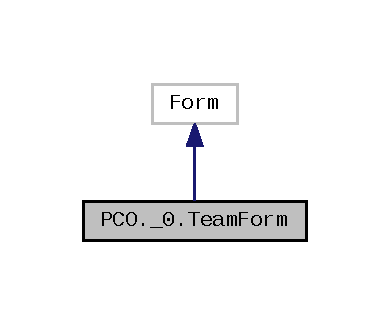
\includegraphics[width=187pt]{classPCO_1_1__0_1_1TeamForm__inherit__graph}
\end{center}
\end{figure}


Collaboration diagram for P\+C\+O.\+\_\+0.\+Team\+Form\+:\nopagebreak
\begin{figure}[H]
\begin{center}
\leavevmode
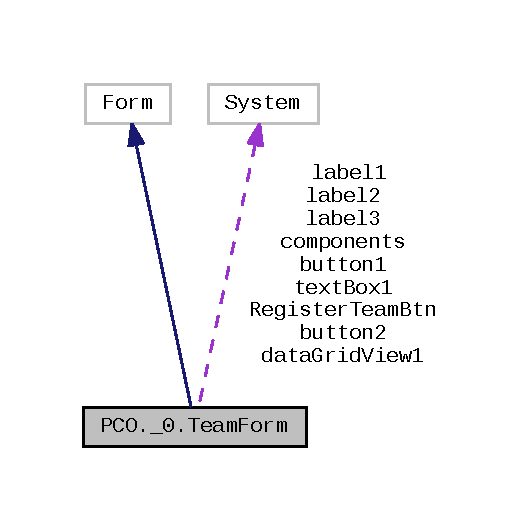
\includegraphics[width=251pt]{classPCO_1_1__0_1_1TeamForm__coll__graph}
\end{center}
\end{figure}
\subsection*{Public Member Functions}
\begin{DoxyCompactItemize}
\item 
\hyperlink{classPCO_1_1__0_1_1TeamForm_a0db8eadd490077e3330e0254ccdc1cee}{Team\+Form} ()
\end{DoxyCompactItemize}
\subsection*{Protected Member Functions}
\begin{DoxyCompactItemize}
\item 
override void \hyperlink{classPCO_1_1__0_1_1TeamForm_a5449a007da7a31beca89946d925d0b69}{Dispose} (bool disposing)
\begin{DoxyCompactList}\small\item\em Clean up any resources being used. \end{DoxyCompactList}\end{DoxyCompactItemize}
\subsection*{Private Member Functions}
\begin{DoxyCompactItemize}
\item 
void \hyperlink{classPCO_1_1__0_1_1TeamForm_a899e959028d070cd6b8f5f66fa02dd39}{Team\+Form\+\_\+\+Load} (object sender, Event\+Args e)
\item 
void \hyperlink{classPCO_1_1__0_1_1TeamForm_add11c999c9095c4ef00332838caba21f}{button1\+\_\+\+Click} (object sender, Event\+Args e)
\item 
void \hyperlink{classPCO_1_1__0_1_1TeamForm_aeec31c575e52aa85997d15790bf8247b}{button1\+\_\+\+Click\+\_\+1} (object sender, Event\+Args e)
\item 
void \hyperlink{classPCO_1_1__0_1_1TeamForm_a22becf6adc591129aab673894df17e50}{label2\+\_\+\+Click} (object sender, Event\+Args e)
\item 
void \hyperlink{classPCO_1_1__0_1_1TeamForm_affe7a93b62d0e51f0bd8ad1cd0e36fe3}{label3\+\_\+\+Click} (object sender, Event\+Args e)
\item 
void \hyperlink{classPCO_1_1__0_1_1TeamForm_a6601c5199799335b1b2056a9ab9ad53c}{text\+Box1\+\_\+\+Text\+Changed} (object sender, Event\+Args e)
\item 
void \hyperlink{classPCO_1_1__0_1_1TeamForm_acfb27ec80635fa1a5bc8c5a7c017e7d8}{data\+Grid\+View1\+\_\+\+Cell\+Content\+Click} (object sender, Data\+Grid\+View\+Cell\+Event\+Args e)
\item 
void \hyperlink{classPCO_1_1__0_1_1TeamForm_ac7fa1fa02781cfe64bdb28ee3f47b35b}{button2\+\_\+\+Click} (object sender, Event\+Args e)
\item 
void \hyperlink{classPCO_1_1__0_1_1TeamForm_a2f95204581542deb466d2c1643aea9d3}{Initialize\+Component} ()
\begin{DoxyCompactList}\small\item\em Required method for Designer support -\/ do not modify the contents of this method with the code editor. \end{DoxyCompactList}\end{DoxyCompactItemize}
\subsection*{Private Attributes}
\begin{DoxyCompactItemize}
\item 
System.\+Component\+Model.\+I\+Container \hyperlink{classPCO_1_1__0_1_1TeamForm_ab5e42668f793e518fe0615bc55ed7cb7}{components} = null
\begin{DoxyCompactList}\small\item\em Required designer variable. \end{DoxyCompactList}\item 
System.\+Windows.\+Forms.\+Data\+Grid\+View \hyperlink{classPCO_1_1__0_1_1TeamForm_a8c2297c2bcd76960ace971955c22284f}{data\+Grid\+View1}
\item 
System.\+Windows.\+Forms.\+Button \hyperlink{classPCO_1_1__0_1_1TeamForm_a77ddf05e8808fb4acf9c781dd7ac1758}{Register\+Team\+Btn}
\item 
System.\+Windows.\+Forms.\+Text\+Box \hyperlink{classPCO_1_1__0_1_1TeamForm_a6c0b69087c958e097e8383236d2470e2}{text\+Box1}
\item 
System.\+Windows.\+Forms.\+Button \hyperlink{classPCO_1_1__0_1_1TeamForm_aeba5f7ade710aabac05af33ab5397254}{button1}
\item 
System.\+Windows.\+Forms.\+Label \hyperlink{classPCO_1_1__0_1_1TeamForm_a0bf7f9e939cb4bea2abbcf798ff1d074}{label1}
\item 
System.\+Windows.\+Forms.\+Label \hyperlink{classPCO_1_1__0_1_1TeamForm_afd83d97a24a823e05306786f062bf285}{label2}
\item 
System.\+Windows.\+Forms.\+Label \hyperlink{classPCO_1_1__0_1_1TeamForm_a7172b2a0037432d76865266b1c33eca9}{label3}
\item 
System.\+Windows.\+Forms.\+Button \hyperlink{classPCO_1_1__0_1_1TeamForm_a15e74530591d8c6cbb7cf9d012e57dee}{button2}
\end{DoxyCompactItemize}


\subsection{Detailed Description}
\hyperlink{classTeam}{Team} class for G\+UI. 

Definition at line 15 of file Team.\+cs.



\subsection{Constructor \& Destructor Documentation}
\mbox{\Hypertarget{classPCO_1_1__0_1_1TeamForm_a0db8eadd490077e3330e0254ccdc1cee}\label{classPCO_1_1__0_1_1TeamForm_a0db8eadd490077e3330e0254ccdc1cee}} 
\index{P\+C\+O\+::\+\_\+0\+::\+Team\+Form@{P\+C\+O\+::\+\_\+0\+::\+Team\+Form}!Team\+Form@{Team\+Form}}
\index{Team\+Form@{Team\+Form}!P\+C\+O\+::\+\_\+0\+::\+Team\+Form@{P\+C\+O\+::\+\_\+0\+::\+Team\+Form}}
\subsubsection{\texorpdfstring{Team\+Form()}{TeamForm()}}
{\footnotesize\ttfamily P\+C\+O.\+\_\+0.\+Team\+Form.\+Team\+Form (\begin{DoxyParamCaption}{ }\end{DoxyParamCaption})\hspace{0.3cm}{\ttfamily [inline]}}



Definition at line 17 of file Team.\+cs.



\subsection{Member Function Documentation}
\mbox{\Hypertarget{classPCO_1_1__0_1_1TeamForm_add11c999c9095c4ef00332838caba21f}\label{classPCO_1_1__0_1_1TeamForm_add11c999c9095c4ef00332838caba21f}} 
\index{P\+C\+O\+::\+\_\+0\+::\+Team\+Form@{P\+C\+O\+::\+\_\+0\+::\+Team\+Form}!button1\+\_\+\+Click@{button1\+\_\+\+Click}}
\index{button1\+\_\+\+Click@{button1\+\_\+\+Click}!P\+C\+O\+::\+\_\+0\+::\+Team\+Form@{P\+C\+O\+::\+\_\+0\+::\+Team\+Form}}
\subsubsection{\texorpdfstring{button1\+\_\+\+Click()}{button1\_Click()}}
{\footnotesize\ttfamily void P\+C\+O.\+\_\+0.\+Team\+Form.\+button1\+\_\+\+Click (\begin{DoxyParamCaption}\item[{object}]{sender,  }\item[{Event\+Args}]{e }\end{DoxyParamCaption})\hspace{0.3cm}{\ttfamily [inline]}, {\ttfamily [private]}}



Definition at line 49 of file Team.\+cs.

\mbox{\Hypertarget{classPCO_1_1__0_1_1TeamForm_aeec31c575e52aa85997d15790bf8247b}\label{classPCO_1_1__0_1_1TeamForm_aeec31c575e52aa85997d15790bf8247b}} 
\index{P\+C\+O\+::\+\_\+0\+::\+Team\+Form@{P\+C\+O\+::\+\_\+0\+::\+Team\+Form}!button1\+\_\+\+Click\+\_\+1@{button1\+\_\+\+Click\+\_\+1}}
\index{button1\+\_\+\+Click\+\_\+1@{button1\+\_\+\+Click\+\_\+1}!P\+C\+O\+::\+\_\+0\+::\+Team\+Form@{P\+C\+O\+::\+\_\+0\+::\+Team\+Form}}
\subsubsection{\texorpdfstring{button1\+\_\+\+Click\+\_\+1()}{button1\_Click\_1()}}
{\footnotesize\ttfamily void P\+C\+O.\+\_\+0.\+Team\+Form.\+button1\+\_\+\+Click\+\_\+1 (\begin{DoxyParamCaption}\item[{object}]{sender,  }\item[{Event\+Args}]{e }\end{DoxyParamCaption})\hspace{0.3cm}{\ttfamily [inline]}, {\ttfamily [private]}}



Definition at line 84 of file Team.\+cs.

\mbox{\Hypertarget{classPCO_1_1__0_1_1TeamForm_ac7fa1fa02781cfe64bdb28ee3f47b35b}\label{classPCO_1_1__0_1_1TeamForm_ac7fa1fa02781cfe64bdb28ee3f47b35b}} 
\index{P\+C\+O\+::\+\_\+0\+::\+Team\+Form@{P\+C\+O\+::\+\_\+0\+::\+Team\+Form}!button2\+\_\+\+Click@{button2\+\_\+\+Click}}
\index{button2\+\_\+\+Click@{button2\+\_\+\+Click}!P\+C\+O\+::\+\_\+0\+::\+Team\+Form@{P\+C\+O\+::\+\_\+0\+::\+Team\+Form}}
\subsubsection{\texorpdfstring{button2\+\_\+\+Click()}{button2\_Click()}}
{\footnotesize\ttfamily void P\+C\+O.\+\_\+0.\+Team\+Form.\+button2\+\_\+\+Click (\begin{DoxyParamCaption}\item[{object}]{sender,  }\item[{Event\+Args}]{e }\end{DoxyParamCaption})\hspace{0.3cm}{\ttfamily [inline]}, {\ttfamily [private]}}



Definition at line 163 of file Team.\+cs.

\mbox{\Hypertarget{classPCO_1_1__0_1_1TeamForm_acfb27ec80635fa1a5bc8c5a7c017e7d8}\label{classPCO_1_1__0_1_1TeamForm_acfb27ec80635fa1a5bc8c5a7c017e7d8}} 
\index{P\+C\+O\+::\+\_\+0\+::\+Team\+Form@{P\+C\+O\+::\+\_\+0\+::\+Team\+Form}!data\+Grid\+View1\+\_\+\+Cell\+Content\+Click@{data\+Grid\+View1\+\_\+\+Cell\+Content\+Click}}
\index{data\+Grid\+View1\+\_\+\+Cell\+Content\+Click@{data\+Grid\+View1\+\_\+\+Cell\+Content\+Click}!P\+C\+O\+::\+\_\+0\+::\+Team\+Form@{P\+C\+O\+::\+\_\+0\+::\+Team\+Form}}
\subsubsection{\texorpdfstring{data\+Grid\+View1\+\_\+\+Cell\+Content\+Click()}{dataGridView1\_CellContentClick()}}
{\footnotesize\ttfamily void P\+C\+O.\+\_\+0.\+Team\+Form.\+data\+Grid\+View1\+\_\+\+Cell\+Content\+Click (\begin{DoxyParamCaption}\item[{object}]{sender,  }\item[{Data\+Grid\+View\+Cell\+Event\+Args}]{e }\end{DoxyParamCaption})\hspace{0.3cm}{\ttfamily [inline]}, {\ttfamily [private]}}



Definition at line 158 of file Team.\+cs.

\mbox{\Hypertarget{classPCO_1_1__0_1_1TeamForm_a5449a007da7a31beca89946d925d0b69}\label{classPCO_1_1__0_1_1TeamForm_a5449a007da7a31beca89946d925d0b69}} 
\index{P\+C\+O\+::\+\_\+0\+::\+Team\+Form@{P\+C\+O\+::\+\_\+0\+::\+Team\+Form}!Dispose@{Dispose}}
\index{Dispose@{Dispose}!P\+C\+O\+::\+\_\+0\+::\+Team\+Form@{P\+C\+O\+::\+\_\+0\+::\+Team\+Form}}
\subsubsection{\texorpdfstring{Dispose()}{Dispose()}}
{\footnotesize\ttfamily override void P\+C\+O.\+\_\+0.\+Team\+Form.\+Dispose (\begin{DoxyParamCaption}\item[{bool}]{disposing }\end{DoxyParamCaption})\hspace{0.3cm}{\ttfamily [inline]}, {\ttfamily [protected]}}



Clean up any resources being used. 


\begin{DoxyParams}{Parameters}
{\em disposing} & true if managed resources should be disposed; otherwise, false.\\
\hline
\end{DoxyParams}


Definition at line 14 of file Team.\+Designer.\+cs.

\mbox{\Hypertarget{classPCO_1_1__0_1_1TeamForm_a2f95204581542deb466d2c1643aea9d3}\label{classPCO_1_1__0_1_1TeamForm_a2f95204581542deb466d2c1643aea9d3}} 
\index{P\+C\+O\+::\+\_\+0\+::\+Team\+Form@{P\+C\+O\+::\+\_\+0\+::\+Team\+Form}!Initialize\+Component@{Initialize\+Component}}
\index{Initialize\+Component@{Initialize\+Component}!P\+C\+O\+::\+\_\+0\+::\+Team\+Form@{P\+C\+O\+::\+\_\+0\+::\+Team\+Form}}
\subsubsection{\texorpdfstring{Initialize\+Component()}{InitializeComponent()}}
{\footnotesize\ttfamily void P\+C\+O.\+\_\+0.\+Team\+Form.\+Initialize\+Component (\begin{DoxyParamCaption}{ }\end{DoxyParamCaption})\hspace{0.3cm}{\ttfamily [inline]}, {\ttfamily [private]}}



Required method for Designer support -\/ do not modify the contents of this method with the code editor. 



Definition at line 29 of file Team.\+Designer.\+cs.

\mbox{\Hypertarget{classPCO_1_1__0_1_1TeamForm_a22becf6adc591129aab673894df17e50}\label{classPCO_1_1__0_1_1TeamForm_a22becf6adc591129aab673894df17e50}} 
\index{P\+C\+O\+::\+\_\+0\+::\+Team\+Form@{P\+C\+O\+::\+\_\+0\+::\+Team\+Form}!label2\+\_\+\+Click@{label2\+\_\+\+Click}}
\index{label2\+\_\+\+Click@{label2\+\_\+\+Click}!P\+C\+O\+::\+\_\+0\+::\+Team\+Form@{P\+C\+O\+::\+\_\+0\+::\+Team\+Form}}
\subsubsection{\texorpdfstring{label2\+\_\+\+Click()}{label2\_Click()}}
{\footnotesize\ttfamily void P\+C\+O.\+\_\+0.\+Team\+Form.\+label2\+\_\+\+Click (\begin{DoxyParamCaption}\item[{object}]{sender,  }\item[{Event\+Args}]{e }\end{DoxyParamCaption})\hspace{0.3cm}{\ttfamily [inline]}, {\ttfamily [private]}}



Definition at line 143 of file Team.\+cs.

\mbox{\Hypertarget{classPCO_1_1__0_1_1TeamForm_affe7a93b62d0e51f0bd8ad1cd0e36fe3}\label{classPCO_1_1__0_1_1TeamForm_affe7a93b62d0e51f0bd8ad1cd0e36fe3}} 
\index{P\+C\+O\+::\+\_\+0\+::\+Team\+Form@{P\+C\+O\+::\+\_\+0\+::\+Team\+Form}!label3\+\_\+\+Click@{label3\+\_\+\+Click}}
\index{label3\+\_\+\+Click@{label3\+\_\+\+Click}!P\+C\+O\+::\+\_\+0\+::\+Team\+Form@{P\+C\+O\+::\+\_\+0\+::\+Team\+Form}}
\subsubsection{\texorpdfstring{label3\+\_\+\+Click()}{label3\_Click()}}
{\footnotesize\ttfamily void P\+C\+O.\+\_\+0.\+Team\+Form.\+label3\+\_\+\+Click (\begin{DoxyParamCaption}\item[{object}]{sender,  }\item[{Event\+Args}]{e }\end{DoxyParamCaption})\hspace{0.3cm}{\ttfamily [inline]}, {\ttfamily [private]}}



Definition at line 148 of file Team.\+cs.

\mbox{\Hypertarget{classPCO_1_1__0_1_1TeamForm_a899e959028d070cd6b8f5f66fa02dd39}\label{classPCO_1_1__0_1_1TeamForm_a899e959028d070cd6b8f5f66fa02dd39}} 
\index{P\+C\+O\+::\+\_\+0\+::\+Team\+Form@{P\+C\+O\+::\+\_\+0\+::\+Team\+Form}!Team\+Form\+\_\+\+Load@{Team\+Form\+\_\+\+Load}}
\index{Team\+Form\+\_\+\+Load@{Team\+Form\+\_\+\+Load}!P\+C\+O\+::\+\_\+0\+::\+Team\+Form@{P\+C\+O\+::\+\_\+0\+::\+Team\+Form}}
\subsubsection{\texorpdfstring{Team\+Form\+\_\+\+Load()}{TeamForm\_Load()}}
{\footnotesize\ttfamily void P\+C\+O.\+\_\+0.\+Team\+Form.\+Team\+Form\+\_\+\+Load (\begin{DoxyParamCaption}\item[{object}]{sender,  }\item[{Event\+Args}]{e }\end{DoxyParamCaption})\hspace{0.3cm}{\ttfamily [inline]}, {\ttfamily [private]}}



Definition at line 22 of file Team.\+cs.

\mbox{\Hypertarget{classPCO_1_1__0_1_1TeamForm_a6601c5199799335b1b2056a9ab9ad53c}\label{classPCO_1_1__0_1_1TeamForm_a6601c5199799335b1b2056a9ab9ad53c}} 
\index{P\+C\+O\+::\+\_\+0\+::\+Team\+Form@{P\+C\+O\+::\+\_\+0\+::\+Team\+Form}!text\+Box1\+\_\+\+Text\+Changed@{text\+Box1\+\_\+\+Text\+Changed}}
\index{text\+Box1\+\_\+\+Text\+Changed@{text\+Box1\+\_\+\+Text\+Changed}!P\+C\+O\+::\+\_\+0\+::\+Team\+Form@{P\+C\+O\+::\+\_\+0\+::\+Team\+Form}}
\subsubsection{\texorpdfstring{text\+Box1\+\_\+\+Text\+Changed()}{textBox1\_TextChanged()}}
{\footnotesize\ttfamily void P\+C\+O.\+\_\+0.\+Team\+Form.\+text\+Box1\+\_\+\+Text\+Changed (\begin{DoxyParamCaption}\item[{object}]{sender,  }\item[{Event\+Args}]{e }\end{DoxyParamCaption})\hspace{0.3cm}{\ttfamily [inline]}, {\ttfamily [private]}}



Definition at line 153 of file Team.\+cs.



\subsection{Member Data Documentation}
\mbox{\Hypertarget{classPCO_1_1__0_1_1TeamForm_aeba5f7ade710aabac05af33ab5397254}\label{classPCO_1_1__0_1_1TeamForm_aeba5f7ade710aabac05af33ab5397254}} 
\index{P\+C\+O\+::\+\_\+0\+::\+Team\+Form@{P\+C\+O\+::\+\_\+0\+::\+Team\+Form}!button1@{button1}}
\index{button1@{button1}!P\+C\+O\+::\+\_\+0\+::\+Team\+Form@{P\+C\+O\+::\+\_\+0\+::\+Team\+Form}}
\subsubsection{\texorpdfstring{button1}{button1}}
{\footnotesize\ttfamily System.\+Windows.\+Forms.\+Button P\+C\+O.\+\_\+0.\+Team\+Form.\+button1\hspace{0.3cm}{\ttfamily [private]}}



Definition at line 146 of file Team.\+Designer.\+cs.

\mbox{\Hypertarget{classPCO_1_1__0_1_1TeamForm_a15e74530591d8c6cbb7cf9d012e57dee}\label{classPCO_1_1__0_1_1TeamForm_a15e74530591d8c6cbb7cf9d012e57dee}} 
\index{P\+C\+O\+::\+\_\+0\+::\+Team\+Form@{P\+C\+O\+::\+\_\+0\+::\+Team\+Form}!button2@{button2}}
\index{button2@{button2}!P\+C\+O\+::\+\_\+0\+::\+Team\+Form@{P\+C\+O\+::\+\_\+0\+::\+Team\+Form}}
\subsubsection{\texorpdfstring{button2}{button2}}
{\footnotesize\ttfamily System.\+Windows.\+Forms.\+Button P\+C\+O.\+\_\+0.\+Team\+Form.\+button2\hspace{0.3cm}{\ttfamily [private]}}



Definition at line 150 of file Team.\+Designer.\+cs.

\mbox{\Hypertarget{classPCO_1_1__0_1_1TeamForm_ab5e42668f793e518fe0615bc55ed7cb7}\label{classPCO_1_1__0_1_1TeamForm_ab5e42668f793e518fe0615bc55ed7cb7}} 
\index{P\+C\+O\+::\+\_\+0\+::\+Team\+Form@{P\+C\+O\+::\+\_\+0\+::\+Team\+Form}!components@{components}}
\index{components@{components}!P\+C\+O\+::\+\_\+0\+::\+Team\+Form@{P\+C\+O\+::\+\_\+0\+::\+Team\+Form}}
\subsubsection{\texorpdfstring{components}{components}}
{\footnotesize\ttfamily System.\+Component\+Model.\+I\+Container P\+C\+O.\+\_\+0.\+Team\+Form.\+components = null\hspace{0.3cm}{\ttfamily [private]}}



Required designer variable. 



Definition at line 8 of file Team.\+Designer.\+cs.

\mbox{\Hypertarget{classPCO_1_1__0_1_1TeamForm_a8c2297c2bcd76960ace971955c22284f}\label{classPCO_1_1__0_1_1TeamForm_a8c2297c2bcd76960ace971955c22284f}} 
\index{P\+C\+O\+::\+\_\+0\+::\+Team\+Form@{P\+C\+O\+::\+\_\+0\+::\+Team\+Form}!data\+Grid\+View1@{data\+Grid\+View1}}
\index{data\+Grid\+View1@{data\+Grid\+View1}!P\+C\+O\+::\+\_\+0\+::\+Team\+Form@{P\+C\+O\+::\+\_\+0\+::\+Team\+Form}}
\subsubsection{\texorpdfstring{data\+Grid\+View1}{dataGridView1}}
{\footnotesize\ttfamily System.\+Windows.\+Forms.\+Data\+Grid\+View P\+C\+O.\+\_\+0.\+Team\+Form.\+data\+Grid\+View1\hspace{0.3cm}{\ttfamily [private]}}



Definition at line 143 of file Team.\+Designer.\+cs.

\mbox{\Hypertarget{classPCO_1_1__0_1_1TeamForm_a0bf7f9e939cb4bea2abbcf798ff1d074}\label{classPCO_1_1__0_1_1TeamForm_a0bf7f9e939cb4bea2abbcf798ff1d074}} 
\index{P\+C\+O\+::\+\_\+0\+::\+Team\+Form@{P\+C\+O\+::\+\_\+0\+::\+Team\+Form}!label1@{label1}}
\index{label1@{label1}!P\+C\+O\+::\+\_\+0\+::\+Team\+Form@{P\+C\+O\+::\+\_\+0\+::\+Team\+Form}}
\subsubsection{\texorpdfstring{label1}{label1}}
{\footnotesize\ttfamily System.\+Windows.\+Forms.\+Label P\+C\+O.\+\_\+0.\+Team\+Form.\+label1\hspace{0.3cm}{\ttfamily [private]}}



Definition at line 147 of file Team.\+Designer.\+cs.

\mbox{\Hypertarget{classPCO_1_1__0_1_1TeamForm_afd83d97a24a823e05306786f062bf285}\label{classPCO_1_1__0_1_1TeamForm_afd83d97a24a823e05306786f062bf285}} 
\index{P\+C\+O\+::\+\_\+0\+::\+Team\+Form@{P\+C\+O\+::\+\_\+0\+::\+Team\+Form}!label2@{label2}}
\index{label2@{label2}!P\+C\+O\+::\+\_\+0\+::\+Team\+Form@{P\+C\+O\+::\+\_\+0\+::\+Team\+Form}}
\subsubsection{\texorpdfstring{label2}{label2}}
{\footnotesize\ttfamily System.\+Windows.\+Forms.\+Label P\+C\+O.\+\_\+0.\+Team\+Form.\+label2\hspace{0.3cm}{\ttfamily [private]}}



Definition at line 148 of file Team.\+Designer.\+cs.

\mbox{\Hypertarget{classPCO_1_1__0_1_1TeamForm_a7172b2a0037432d76865266b1c33eca9}\label{classPCO_1_1__0_1_1TeamForm_a7172b2a0037432d76865266b1c33eca9}} 
\index{P\+C\+O\+::\+\_\+0\+::\+Team\+Form@{P\+C\+O\+::\+\_\+0\+::\+Team\+Form}!label3@{label3}}
\index{label3@{label3}!P\+C\+O\+::\+\_\+0\+::\+Team\+Form@{P\+C\+O\+::\+\_\+0\+::\+Team\+Form}}
\subsubsection{\texorpdfstring{label3}{label3}}
{\footnotesize\ttfamily System.\+Windows.\+Forms.\+Label P\+C\+O.\+\_\+0.\+Team\+Form.\+label3\hspace{0.3cm}{\ttfamily [private]}}



Definition at line 149 of file Team.\+Designer.\+cs.

\mbox{\Hypertarget{classPCO_1_1__0_1_1TeamForm_a77ddf05e8808fb4acf9c781dd7ac1758}\label{classPCO_1_1__0_1_1TeamForm_a77ddf05e8808fb4acf9c781dd7ac1758}} 
\index{P\+C\+O\+::\+\_\+0\+::\+Team\+Form@{P\+C\+O\+::\+\_\+0\+::\+Team\+Form}!Register\+Team\+Btn@{Register\+Team\+Btn}}
\index{Register\+Team\+Btn@{Register\+Team\+Btn}!P\+C\+O\+::\+\_\+0\+::\+Team\+Form@{P\+C\+O\+::\+\_\+0\+::\+Team\+Form}}
\subsubsection{\texorpdfstring{Register\+Team\+Btn}{RegisterTeamBtn}}
{\footnotesize\ttfamily System.\+Windows.\+Forms.\+Button P\+C\+O.\+\_\+0.\+Team\+Form.\+Register\+Team\+Btn\hspace{0.3cm}{\ttfamily [private]}}



Definition at line 144 of file Team.\+Designer.\+cs.

\mbox{\Hypertarget{classPCO_1_1__0_1_1TeamForm_a6c0b69087c958e097e8383236d2470e2}\label{classPCO_1_1__0_1_1TeamForm_a6c0b69087c958e097e8383236d2470e2}} 
\index{P\+C\+O\+::\+\_\+0\+::\+Team\+Form@{P\+C\+O\+::\+\_\+0\+::\+Team\+Form}!text\+Box1@{text\+Box1}}
\index{text\+Box1@{text\+Box1}!P\+C\+O\+::\+\_\+0\+::\+Team\+Form@{P\+C\+O\+::\+\_\+0\+::\+Team\+Form}}
\subsubsection{\texorpdfstring{text\+Box1}{textBox1}}
{\footnotesize\ttfamily System.\+Windows.\+Forms.\+Text\+Box P\+C\+O.\+\_\+0.\+Team\+Form.\+text\+Box1\hspace{0.3cm}{\ttfamily [private]}}



Definition at line 145 of file Team.\+Designer.\+cs.



The documentation for this class was generated from the following files\+:\begin{DoxyCompactItemize}
\item 
\hyperlink{Team_8cs}{Team.\+cs}\item 
\hyperlink{Team_8Designer_8cs}{Team.\+Designer.\+cs}\end{DoxyCompactItemize}

\chapter{File Documentation}
\hypertarget{Class1_8cs}{}\section{Class1.\+cs File Reference}
\label{Class1_8cs}\index{Class1.\+cs@{Class1.\+cs}}
\subsection*{Classes}
\begin{DoxyCompactItemize}
\item 
class \hyperlink{classAthlete}{Athlete}
\begin{DoxyCompactList}\small\item\em \hyperlink{classAthlete}{Athlete} class to input individual\textquotesingle{}s personal information and events to partake in. \end{DoxyCompactList}\item 
class \hyperlink{classDatabase}{Database}
\begin{DoxyCompactList}\small\item\em D\+E\+P\+R\+E\+C\+A\+T\+E\+D!!! \hyperlink{classDatabase}{Database} S\+U\+B\+S\+Y\+S\+T\+EM houses all the information of the Winter Olympics. \end{DoxyCompactList}\item 
class \hyperlink{classIceDance}{Ice\+Dance}
\begin{DoxyCompactList}\small\item\em \hyperlink{classIceDance}{Ice\+Dance} class is one of the 3 Figure\+Skating events. \end{DoxyCompactList}\item 
class \hyperlink{classRegistration}{Registration}
\begin{DoxyCompactList}\small\item\em \hyperlink{classRegistration}{Registration} class registers Teams and Athletes. \end{DoxyCompactList}\item 
class \hyperlink{classSS1000m}{S\+S1000m}
\begin{DoxyCompactList}\small\item\em \hyperlink{classSS1000m}{S\+S1000m} is one of the 3 Speed\+Skating events. \end{DoxyCompactList}\item 
class \hyperlink{classSS1500m}{S\+S1500m}
\begin{DoxyCompactList}\small\item\em \hyperlink{classSS1500m}{S\+S1500m} is one of the 3 Speed\+Skating events. \end{DoxyCompactList}\item 
class \hyperlink{classSS500m}{S\+S500m}
\begin{DoxyCompactList}\small\item\em \hyperlink{classSS500m}{S\+S500m} is one of the 3 Speed\+Skating events. \end{DoxyCompactList}\item 
class \hyperlink{classScoring}{Scoring}
\begin{DoxyCompactList}\small\item\em \hyperlink{classScoring}{Scoring} class manages the official scores/times recorded by the judges. \end{DoxyCompactList}\item 
class \hyperlink{classSingleSkating}{Single\+Skating}
\begin{DoxyCompactList}\small\item\em \hyperlink{classSingleSkating}{Single\+Skating} class is one of the 3 Figure\+Skating events. \end{DoxyCompactList}\item 
class \hyperlink{classPairSkating}{Pair\+Skating}
\begin{DoxyCompactList}\small\item\em \hyperlink{classPairSkating}{Pair\+Skating} class is one of the 3 Figure\+Skating events. \end{DoxyCompactList}\item 
class \hyperlink{classTeam}{Team}
\begin{DoxyCompactList}\small\item\em \hyperlink{classTeam}{Team} class to house the team name. \end{DoxyCompactList}\end{DoxyCompactItemize}

\hypertarget{Display_8cs}{}\section{Display.\+cs File Reference}
\label{Display_8cs}\index{Display.\+cs@{Display.\+cs}}
\subsection*{Classes}
\begin{DoxyCompactItemize}
\item 
class \hyperlink{classPCO_1_1Display}{P\+C\+O.\+Display}
\begin{DoxyCompactList}\small\item\em \hyperlink{classPCO_1_1Display}{Display} class for G\+UI. \end{DoxyCompactList}\end{DoxyCompactItemize}
\subsection*{Namespaces}
\begin{DoxyCompactItemize}
\item 
namespace \hyperlink{namespacePCO}{P\+CO}
\end{DoxyCompactItemize}

\hypertarget{Display_8Designer_8cs}{}\section{Display.\+Designer.\+cs File Reference}
\label{Display_8Designer_8cs}\index{Display.\+Designer.\+cs@{Display.\+Designer.\+cs}}
\subsection*{Classes}
\begin{DoxyCompactItemize}
\item 
class \hyperlink{classPCO_1_1__0_1_1Display}{P\+C\+O.\+\_\+0.\+Display}
\begin{DoxyCompactList}\small\item\em \hyperlink{classPCO_1_1__0_1_1Display}{Display} class for G\+UI. \end{DoxyCompactList}\end{DoxyCompactItemize}
\subsection*{Namespaces}
\begin{DoxyCompactItemize}
\item 
namespace \hyperlink{namespacePCO_1_1__0}{P\+C\+O.\+\_\+0}
\end{DoxyCompactItemize}

\hypertarget{Event_8cs}{}\section{Event.\+cs File Reference}
\label{Event_8cs}\index{Event.\+cs@{Event.\+cs}}
\subsection*{Classes}
\begin{DoxyCompactItemize}
\item 
class \hyperlink{classPCO_1_1__0_1_1RegisterEventForm}{P\+C\+O.\+\_\+0.\+Register\+Event\+Form}
\begin{DoxyCompactList}\small\item\em Register Event class for G\+UI. \end{DoxyCompactList}\end{DoxyCompactItemize}
\subsection*{Namespaces}
\begin{DoxyCompactItemize}
\item 
namespace \hyperlink{namespacePCO_1_1__0}{P\+C\+O.\+\_\+0}
\end{DoxyCompactItemize}

\hypertarget{Event_8Designer_8cs}{}\section{Event.\+Designer.\+cs File Reference}
\label{Event_8Designer_8cs}\index{Event.\+Designer.\+cs@{Event.\+Designer.\+cs}}
\subsection*{Classes}
\begin{DoxyCompactItemize}
\item 
class \hyperlink{classPCO_1_1RegisterEventForm}{P\+C\+O.\+Register\+Event\+Form}
\begin{DoxyCompactList}\small\item\em Register Event class for G\+UI. \end{DoxyCompactList}\end{DoxyCompactItemize}
\subsection*{Namespaces}
\begin{DoxyCompactItemize}
\item 
namespace \hyperlink{namespacePCO}{P\+CO}
\end{DoxyCompactItemize}

\hypertarget{Form1_8cs}{}\section{Form1.\+cs File Reference}
\label{Form1_8cs}\index{Form1.\+cs@{Form1.\+cs}}
\subsection*{Classes}
\begin{DoxyCompactItemize}
\item 
class \hyperlink{classPCO_1_1__0_1_1Form1}{P\+C\+O.\+\_\+0.\+Form1}
\begin{DoxyCompactList}\small\item\em Main Screen class for G\+UI. \end{DoxyCompactList}\end{DoxyCompactItemize}
\subsection*{Namespaces}
\begin{DoxyCompactItemize}
\item 
namespace \hyperlink{namespacePCO_1_1__0}{P\+C\+O.\+\_\+0}
\end{DoxyCompactItemize}

\hypertarget{Form1_8Designer_8cs}{}\section{Form1.\+Designer.\+cs File Reference}
\label{Form1_8Designer_8cs}\index{Form1.\+Designer.\+cs@{Form1.\+Designer.\+cs}}
\subsection*{Classes}
\begin{DoxyCompactItemize}
\item 
class \hyperlink{classPCO_1_1__0_1_1Form1}{P\+C\+O.\+\_\+0.\+Form1}
\begin{DoxyCompactList}\small\item\em Main Screen class for G\+UI. \end{DoxyCompactList}\end{DoxyCompactItemize}
\subsection*{Namespaces}
\begin{DoxyCompactItemize}
\item 
namespace \hyperlink{namespacePCO_1_1__0}{P\+C\+O.\+\_\+0}
\end{DoxyCompactItemize}

\hypertarget{Judge_8cs}{}\section{Judge.\+cs File Reference}
\label{Judge_8cs}\index{Judge.\+cs@{Judge.\+cs}}
\subsection*{Classes}
\begin{DoxyCompactItemize}
\item 
class \hyperlink{classPCO_1_1ScoringForm}{P\+C\+O.\+Scoring\+Form}
\begin{DoxyCompactList}\small\item\em \hyperlink{classScoring}{Scoring} class for G\+UI. \end{DoxyCompactList}\end{DoxyCompactItemize}
\subsection*{Namespaces}
\begin{DoxyCompactItemize}
\item 
namespace \hyperlink{namespacePCO}{P\+CO}
\end{DoxyCompactItemize}

\hypertarget{Judge_8Designer_8cs}{}\section{Judge.\+Designer.\+cs File Reference}
\label{Judge_8Designer_8cs}\index{Judge.\+Designer.\+cs@{Judge.\+Designer.\+cs}}
\subsection*{Classes}
\begin{DoxyCompactItemize}
\item 
class \hyperlink{classPCO_1_1__0_1_1ScoringForm}{P\+C\+O.\+\_\+0.\+Scoring\+Form}
\begin{DoxyCompactList}\small\item\em \hyperlink{classScoring}{Scoring} class for G\+UI. \end{DoxyCompactList}\end{DoxyCompactItemize}
\subsection*{Namespaces}
\begin{DoxyCompactItemize}
\item 
namespace \hyperlink{namespacePCO_1_1__0}{P\+C\+O.\+\_\+0}
\end{DoxyCompactItemize}

\hypertarget{Program_8cs}{}\section{Program.\+cs File Reference}
\label{Program_8cs}\index{Program.\+cs@{Program.\+cs}}
\subsection*{Classes}
\begin{DoxyCompactItemize}
\item 
class {\bfseries P\+C\+O.\+Program}
\end{DoxyCompactItemize}
\subsection*{Namespaces}
\begin{DoxyCompactItemize}
\item 
namespace \hyperlink{namespacePCO}{P\+CO}
\end{DoxyCompactItemize}

\hypertarget{Registration_8cs}{}\section{Registration.\+cs File Reference}
\label{Registration_8cs}\index{Registration.\+cs@{Registration.\+cs}}
\subsection*{Classes}
\begin{DoxyCompactItemize}
\item 
class \hyperlink{classPCO_1_1__0_1_1AthleteForm}{P\+C\+O.\+\_\+0.\+Athlete\+Form}
\begin{DoxyCompactList}\small\item\em \hyperlink{classRegistration}{Registration} class for G\+UI. \end{DoxyCompactList}\end{DoxyCompactItemize}
\subsection*{Namespaces}
\begin{DoxyCompactItemize}
\item 
namespace \hyperlink{namespacePCO_1_1__0}{P\+C\+O.\+\_\+0}
\end{DoxyCompactItemize}

\hypertarget{Registration_8Designer_8cs}{}\section{Registration.\+Designer.\+cs File Reference}
\label{Registration_8Designer_8cs}\index{Registration.\+Designer.\+cs@{Registration.\+Designer.\+cs}}
\subsection*{Classes}
\begin{DoxyCompactItemize}
\item 
class \hyperlink{classPCO_1_1AthleteForm}{P\+C\+O.\+Athlete\+Form}
\begin{DoxyCompactList}\small\item\em \hyperlink{classRegistration}{Registration} class for G\+UI. \end{DoxyCompactList}\end{DoxyCompactItemize}
\subsection*{Namespaces}
\begin{DoxyCompactItemize}
\item 
namespace \hyperlink{namespacePCO}{P\+CO}
\end{DoxyCompactItemize}

\hypertarget{Team_8cs}{}\section{Team.\+cs File Reference}
\label{Team_8cs}\index{Team.\+cs@{Team.\+cs}}
\subsection*{Classes}
\begin{DoxyCompactItemize}
\item 
class \hyperlink{classPCO_1_1__0_1_1TeamForm}{P\+C\+O.\+\_\+0.\+Team\+Form}
\begin{DoxyCompactList}\small\item\em \hyperlink{classTeam}{Team} class for G\+UI. \end{DoxyCompactList}\end{DoxyCompactItemize}
\subsection*{Namespaces}
\begin{DoxyCompactItemize}
\item 
namespace \hyperlink{namespacePCO_1_1__0}{P\+C\+O.\+\_\+0}
\end{DoxyCompactItemize}

\hypertarget{Team_8Designer_8cs}{}\section{Team.\+Designer.\+cs File Reference}
\label{Team_8Designer_8cs}\index{Team.\+Designer.\+cs@{Team.\+Designer.\+cs}}
\subsection*{Classes}
\begin{DoxyCompactItemize}
\item 
class \hyperlink{classPCO_1_1TeamForm}{P\+C\+O.\+Team\+Form}
\begin{DoxyCompactList}\small\item\em \hyperlink{classTeam}{Team} class for G\+UI. \end{DoxyCompactList}\end{DoxyCompactItemize}
\subsection*{Namespaces}
\begin{DoxyCompactItemize}
\item 
namespace \hyperlink{namespacePCO}{P\+CO}
\end{DoxyCompactItemize}

%--- End generated contents ---

% Index
\backmatter
\newpage
\phantomsection
\clearemptydoublepage
\addcontentsline{toc}{chapter}{Index}
\printindex

\end{document}
